% main-es.tex — Documento final del proyecto (curso 32310004), español
%
% No hay consigna oficial todavía (intro.md sin consigna), por lo que el documento sigue la
% estructura estándar de un artículo. Cuando llegue la consigna, ese archivo manda y este
% documento se adapta — no al revés.
%
% Guardarraíl de motor: el preámbulo usa fontspec (OpenType). Con pdflatex los
% acentos salen rotos, así que aquí se aborta en vez de emitir un PDF malo.
\RequirePackage{iftex}\RequireXeTeX

\documentclass[12pt,letterpaper]{article}
\newcommand{\docNombre}{Documento final}
% common/preamble.tex — paquetes compartidos por los documentos del curso.
%
% Deliberadamente ligero: el avance es un documento corto de quiz, no una
% tesis. Se carga desde la carpeta de cada documento (avance/, final/), así que
% TODAS las rutas de abajo son relativas al directorio del documento:
%   common/   -> ../common/
%   assets/   -> ../assets/pics/
%   bib/      -> ../bib/refs.bib
% ACOPLAMIENTO: si algo de eso se mueve, la compilación falla (o peor: compila
% sin el logo). No hay script que lo detecte.

% --- Matemáticas (antes de unicode-math, que si no avisa) ---
\usepackage{mathtools}

% --- Fuentes (XeLaTeX) ---
% Libertinus. Se cargan por NOMBRE DE ARCHIVO + Extension, no por nombre de
% familia: en TeXLive las .otf viven en el árbol de texmf y fontconfig no las
% ve, así que \setmainfont{Libertinus Serif} falla.
\usepackage[warnings-off={mathtools-colon,mathtools-overbracket},mathbf=sym]{unicode-math}
\setmainfont{LibertinusSerif}[
  Extension     = .otf,
  UprightFont   = *-Regular,
  ItalicFont    = *-Italic,
  BoldFont      = *-Semibold,
  BoldItalicFont= *-SemiboldItalic,
  Ligatures     = TeX,
]
\setsansfont{LibertinusSans}[
  Extension     = .otf,
  UprightFont   = *-Regular,
  ItalicFont    = *-Italic,
  BoldFont      = *-Bold,
  BoldItalicFont= *-Bold,
  Ligatures     = TeX,
]
\setmathfont{LibertinusMath-Regular.otf}

% --- Idioma ---
% es-noshorthands: los shorthands < > ~ . de babel-spanish rompen cleveref y las
% columnas d{..} de dcolumn.
\usepackage[english,spanish,es-noshorthands]{babel}
\selectlanguage{spanish}

% --- Geometría y espaciado ---
\usepackage[letterpaper,margin=2.5cm]{geometry}
\usepackage{setspace}\onehalfspacing
\usepackage{parskip}

% --- Tablas (los documentos son tabla-pesados: consignas y métricas) ---
\usepackage{booktabs}
\usepackage{longtable}
\usepackage{array}
\usepackage{tabularx}
\usepackage[section]{placeins} % las tablas no pueden flotar fuera de su sección
\newcolumntype{L}[1]{>{\raggedright\arraybackslash}p{#1}}
% Filas menos pegadas: un poco más de aire vertical en todas las tablas.
\renewcommand{\arraystretch}{1.3}
% \sepfilas: separador punteado gris discreto entre filas (booktabs no trae
% líneas punteadas). Va solo tras el \\ de cada fila de cuerpo. colortbl va
% antes de arydshln y le da el \arrayrulecolor (global: se restaura a negro).
\usepackage{colortbl}
\usepackage{arydshln} % último de los paquetes de tabla: su manual lo exige
\newcommand{\sepfilas}{%
  \arrayrulecolor{gray!60}\hdashline[0.8pt/3pt]\arrayrulecolor{black}}

% --- Color, cajas y enlaces ---
\usepackage{xcolor}
\usepackage[most]{tcolorbox}
\usepackage{enumitem}
\usepackage[hidelinks]{hyperref}

% --- Logo institucional: compartido por todos los documentos del curso ---
\usepackage{graphicx}
\graphicspath{{../assets/pics/}}

% --- Comillas dependientes del idioma (biblatex lo exige junto con babel) ---
\usepackage{csquotes}

% --- Bibliografía: UN SOLO refs.bib para todos los entregables del curso ---
\usepackage[backend=biber,style=authoryear,sorting=nyt,maxcitenames=2,
            maxbibnames=99,giveninits=true,uniquename=init,doi=true,url=true,isbn=false]{biblatex}
\addbibresource{../bib/refs.bib}

% common/macros.tex — dos macros de ayuda, compartidos por todos los documentos
% del curso (avance, final).

% ---------------------------------------------------------------------------
% Modo FINAL: `make es FINAL=1` crea el archivo .final-mode y las cajas de ayuda
% desaparecen. El flag lo busca ESTE archivo con \IfFileExists, así que es
% relativo al directorio desde donde compila latexmk (la carpeta del documento).
% ---------------------------------------------------------------------------
\newif\ifdocFinal \docFinalfalse
\IfFileExists{.final-mode}{\docFinaltrue}{}

% ---------------------------------------------------------------------------
% \limite{N}{qué pide la consigna aquí}
%
% Caja al inicio de cada sección con el presupuesto de palabras y el texto
% literal de la consigna (intro.md en el avance, formulario oficial en el
% final). Visible en borrador, invisible en FINAL.
% N = 0 significa "sin límite declarado".
% ---------------------------------------------------------------------------
\newcommand{\limite}[2]{%
  \ifdocFinal\else
    \begin{tcolorbox}[
      colback=blue!3, colframe=blue!35, boxrule=0.4pt,
      left=6pt, right=6pt, top=4pt, bottom=4pt,
      before skip=6pt, after skip=10pt]
      \footnotesize
      \ifnum#1>0\textbf{Máximo #1 palabras.}\quad\fi
      #2
    \end{tcolorbox}
  \fi
}

% ---------------------------------------------------------------------------
% \nota{...} — recordatorio interno de qué falta o de cómo se conecta con el
% resto del proyecto. Invisible en FINAL.
% ---------------------------------------------------------------------------
\newcommand{\nota}[1]{%
  \ifdocFinal\else
    {\color{orange!70!black}\footnotesize\textsf{[nota: #1]}\par\medskip}
  \fi
}

% ---------------------------------------------------------------------------
% \TODO{...} — dato que todavía no se tiene. Nunca se inventa un dato: se
% marca. En FINAL sigue VISIBLE y en rojo, a propósito: un documento no se
% entrega con campos sin llenar, y el modo final tiene que gritarlo.
% ---------------------------------------------------------------------------
\newcommand{\TODO}[1]{{\color{red}\textbf{[POR DEFINIR: #1]}}}

% common/meta-es.tex — metadatos compartidos por los documentos del curso.
% Todos en un solo sitio. Regla: aquí no se inventa nada; un dato que no se
% tiene de la fuente se deja como \TODO{...} y sale en rojo, también en FINAL.
% El nombre del documento (\docNombre) NO vive aquí: cada main-es.tex lo define,
% porque es lo único que distingue al avance del final.

% ===== Proyecto =====
\newcommand{\proyTitulo}{Planes auto-editables: Lazo abierto vs.\ replanificación}
\newcommand{\proyPregunta}{¿Bajo qué condiciones del entorno un agente que reescribe su propio plan supera a uno con plan estático y desde qué costo de reescritura se invierte esa ventaja?}

% ===== Curso =====
\newcommand{\proyCurso}{Inteligencia Artificial: Representación y Solución de Problemas}
\newcommand{\proyCursoCorto}{IA: Representación y Solución de Problemas}
\newcommand{\proyCodigo}{32310004}
\newcommand{\proyUniversidad}{Universidad del Rosario}

% ===== Gente =====
\newcommand{\proyEstudiante}{Over Haider Castrillón Valencia}
\newcommand{\proyProfesor}{Nicolás Avilán Vargas, Ph.D.}

% ===== Fecha =====
\newcommand{\proyFecha}{\today}


% --- Encabezado de página: nombre del documento (define cada main-es.tex) ---
\providecommand{\docNombre}{Documento}
\usepackage{fancyhdr}
\pagestyle{fancy}\fancyhf{}
\fancyhead[L]{\footnotesize \docNombre{} \textbar{} \proyCursoCorto}
\fancyhead[R]{\footnotesize\thepage}
\renewcommand{\headrulewidth}{0.4pt}

% --- Títulos de sección numerados, al estilo de las consignas del curso ---
\usepackage{titlesec}
\titleformat{\section}{\normalfont\large\bfseries}{\thesection.}{0.5em}{}
\titlespacing*{\section}{0pt}{1.5\baselineskip}{0.5\baselineskip}

% Las figuras salen tal cual las exporta `python -m project.analysis --figuras`.
\graphicspath{{../assets/pics/}{../../results/figuras/}{../../results/animaciones/}}

% --- Macros locales de este documento (no van a common/: solo el final las usa) ---
% Monoespaciada de la misma familia, escalada a la altura de x del texto, para que los
% nombres de política no se vean más grandes que la prosa (ni en tablas \footnotesize).
\setmonofont{LibertinusMono}[Extension=.otf, UprightFont=*-Regular, BoldFont=*-Regular, Scale=MatchLowercase]
% Nombres de las ocho políticas, tal como aparecen en el código y en los CSV.
\newcommand{\pol}[1]{\texttt{#1}}
\newcommand{\RX}{\pol{REFLEX}}
\newcommand{\MB}{\pol{MODEL\_BASED}}
\newcommand{\OL}{\pol{OPEN\_LOOP}}
\newcommand{\CR}{\pol{COLD\_RESTART}}
\newcommand{\CL}{\pol{CLOSED\_LOOP}}
\newcommand{\GOV}{\pol{GOVERNED}}
\newcommand{\KB}{\pol{KNOWLEDGE\_BASED}}
\newcommand{\BY}{\pol{BAYESIAN}}
% Abreviaturas de política para los encabezados de cuadros anchos (ver cuadro de políticas).
\newcommand{\ab}[1]{\pol{#1}}
% Los nombres de política en monoespaciada no se dividen: un poco de holgura evita cajas
% desbordadas en párrafos con varios de ellos.
\setlength{\emergencystretch}{3em}
% Diferencia pareada por semilla: media ± error estándar de la diferencia.
\newcommand{\dif}[2]{$#1 \pm #2$}
% Horizontes de validez del agente basado en conocimiento.
\newcommand{\ahora}{«ahora»}
\newcommand{\llegada}{«llegada»}

\begin{document}

% Las cajas de ayuda no son contenido: texcount las ignora (ver `make wordcount`).
%TC:macro \limite [ignore,ignore]
%TC:macro \nota [ignore]
%TC:macro \TODO [ignore]
\thispagestyle{empty}
\begin{center}
  
\includegraphics[width=3.2cm]{ur-logo}\\[1.2em]
  {\Large\bfseries \docNombre}\\[0.4em]
  {\large \proyCurso{} (\proyCodigo)}\\[0.2em]
  {\normalsize \proyUniversidad}\\[2em]
  {\large\bfseries \proyTitulo}\\[0.4em]
  {\normalsize \itshape \proyPregunta}\\[2.5em]
\end{center}

\begin{center}
\begin{tabular}{@{}>{\bfseries}r l@{}}
Estudiante & \proyEstudiante \\
Profesor   & \proyProfesor \\
Fecha      & \proyFecha \\
\end{tabular}
\end{center}

\vfill
\ifdocFinal\else
\begin{center}
  \footnotesize Compilado con Xe\LaTeX{} (borrador visible): Las notas naranjas son internas y desaparecen con \texttt{make es FINAL=1}.
\end{center}
\fi
\clearpage

% !TEX root = ../main-es.tex
%TC:macro \limite [ignore,ignore]
%TC:macro \nota [ignore]
%TC:macro \TODO [ignore]
%TC:macro \parencite [ignore]
%TC:macro \textcite [ignore]
\section*{Resumen}

Los agentes auto-evolutivos reescriben durante su propia ejecución el plan que los guía, pero la decisión de cuándo hacerlo se toma hoy por intuición. Este trabajo la convierte en una frontera medible mediante un modelo basado en agentes en MESA, en el que un recolector opera sobre una retícula de $15\times15$ cuyos recursos se desplazan con probabilidad $\lambda$ por tick, y en el que reescribir el plan equivale a consultar a un oráculo con competencia $p$ que ocupa $c$ ticks mientras el mundo sigue moviéndose. Se comparan ocho arquitecturas, desde el reflejo simple hasta un agente basado en conocimiento con fluentes y uno bayesiano que aprende $\lambda$ mirando, en 16.260 corridas distribuidas en trece barridos con 30 semillas pareadas, más series temporales y una calibración por computación bayesiana aproximada (ABC).

Con el mismo replanificador al mismo precio, reparar al detectar la divergencia y esperar a que el plan falle casi empatan (en 13 de las 16 celdas dinámicas la diferencia cae dentro de dos errores estándar), mientras que la frontera que sí aparece separa deliberar de no deliberar: Con $\lambda=0.5$ y $c\ge2$, o con $\lambda=0.25$ y $c\ge5$, el agente reactivo basado en modelo supera a toda política que planifica (98.3 contra 53.3 de la mejor con $c=2$), tanto más cuanto más abundan los objetivos. Reparar en caliente supera a reiniciar en frío desde $\lambda=0.1$ (de $+16$ a $+22$ puntos con $c$ entre 2 y 5). El agente lógico supera al lazo cerrado solo porque repara menos (\dif{+21.3}{3.8} con $r=3$ y $\lambda=0.5$), y el bayesiano, aunque su creencia está calibrada, decide peor que él (\dif{-16.0}{4.3}), porque su regla de utilidad esperada repara de más. Finalmente, la calibración por ABC recupera $\lambda$ a partir de la telemetría de un despliegue pero no $p$, lo cual basta para el criterio que se propone, que consiste en medir el dinamismo del entorno y el costo de deliberar antes que la calidad del replanificador.

\medskip
\noindent\textbf{Palabras clave:} agentes auto-evolutivos, monitoreo de ejecución, replanificación, metarazonamiento, modelos basados en agentes, agentes basados en conocimiento, filtrado bayesiano.

\clearpage
{\hypersetup{linkcolor=black}\tableofcontents}
\clearpage

% !TEX root = ../main-es.tex
%TC:macro \limite [ignore,ignore]
%TC:macro \nota [ignore]
%TC:macro \TODO [ignore]
%TC:macro \parencite [ignore]
%TC:macro \textcite [ignore]
\section{Introducción}\label{sec:introduccion}

\subsection{Motivación}

Existe hoy una clase emergente de sistemas a la que la literatura ya le puso nombre, los \emph{agentes auto-evolutivos} \parencite{gao2026selfevolving}, en la que el agente modifica durante su propia ejecución los componentes que lo definen, ya sea el flujo de trabajo que sigue, la memoria que consulta o el programa mismo que lo está ejecutando, de forma que la auto-modificación dejó de ser una especulación teórica para volverse una propiedad de sistemas desplegados. Las instancias de esa clase son públicas y verificables: Voyager programa sus propias habilidades en Minecraft y las repara cuando su verificación falla \parencite{wang2023voyager}, Reflexion reescribe su memoria verbal tras cada fracaso \parencite{shinn2023reflexion}, Agent Workflow Memory induce flujos de trabajo reutilizables mientras opera \parencite{wang2024awm}, y AFlow y ADAS buscan automáticamente, representados como código, el flujo que el agente ejecuta \parencite{zhang2024aflow,hu2024adas}. El caso límite lo documentaron los propios autores de The AI Scientist, cuyo agente editó su código para extenderse el límite de tiempo que lo acotaba y en otra corrida se relanzó a sí mismo \parencite{lu2024aiscientist}, lo cual muestra que la capacidad de reescribirse alcanza ya a las restricciones puestas para contenerla.

El problema es que esa capacidad se despliega sin un criterio medido de cuándo ejercerla, pues los orquestadores actuales fijan por intuición cada cuánto conviene replanificar, y la pregunta por el cuándo sigue abierta en la agenda de la propia clase, que la nombra explícitamente como la dimensión \emph{when} \parencite{gao2026selfevolving}. Este trabajo aborda esa pregunta desde una instancia de calibración concreta, un motor de ejecución agéntica propio (OASys) en el que un agente basado en un modelo de lenguaje puede leer y reescribir el programa que lo ejecuta, y en el que las tres decisiones que importan se resolvieron por intuición: Las ediciones surten efecto en la ejecución siguiente (de modo que el trabajo en curso se pierde), porque nadie sabía si compensaba construir la reparación en caliente; la deliberación se acota con un tope fijo de cinco iteraciones, sin justificación derivada; y el único freno contra un ciclo de reescrituras improductivas es la autorización humana. Vale la pena anotarlo con honestidad: Se trata de un sistema propio y no publicado, de forma que aquí aporta la pregunta y los parámetros que un despliegue real podría medir, pero no evidencia, la cual recae por completo sobre el experimento reproducible que se describe en las secciones siguientes.

Al leer la teoría clásica de agentes con esa instancia en mente resulta que el mecanismo completo ya está descrito con otro vocabulario \parencite{russellNorvig2020}: El programa editable es un plan (jerárquico, §11.4), revisarlo contra lo que se observa es monitoreo de ejecución y reescribirlo es replanificación (§11.5), lo que el agente tiene a la vista es observabilidad parcial (§2.3.2), y aplicar la edición en la ejecución siguiente o sobre la ejecución en curso es la distinción entre planificar en lazo abierto y en lazo cerrado (§11.5). Si el problema es clásico, cabe la pregunta clásica: El beneficio de replanificar crece con el dinamismo del entorno, mientras que su costo (el tiempo durante el cual el agente delibera y el mundo sigue cambiando) es aproximadamente constante, por lo que debería existir un punto de cruce, y es ese punto el que nadie había medido.

\subsection{La pregunta}

\begin{quote}
  \itshape\proyPregunta
\end{quote}

Para responderla se construyó un modelo basado en agentes en MESA \parencite{kazil2020mesa}, en el que un agente recolector reúne recursos que se desplazan sobre una retícula con obstáculos, y en el que la decisión de modelado central es tratar la deliberación como una acción más, que ocupa ticks del reloj durante los cuales el mundo se sigue moviendo. El replanificador no es un modelo de lenguaje real sino un oráculo abstracto con dos parámetros, la competencia $p$ (la probabilidad de que la reparación propuesta sea la óptima) y el costo $c$ (los ticks que tarda en proponerla), cuyos errores son plausibles y no ruido. Cabe mencionar que esa abstracción es una decisión metodológica y no solo de presupuesto, pues convierte una propiedad del modelo de lenguaje en un parámetro del experimento: Con un modelo real solo se puede responder si la auto-edición funcionó con ese modelo en ese momento, mientras que con el oráculo se puede preguntar a partir de qué competencia y de qué costo conviene dejar que un agente se reescriba, que es un enunciado que sobrevive al cambio de modelo.

\subsection{Aportes}

\begin{enumerate}[leftmargin=1.6em, itemsep=0.3em]
  \item \textbf{Un modelo reproducible de la auto-edición de planes,} con ocho arquitecturas que recorren la taxonomía de agentes de \textcite{russellNorvig2020}, desde el reflejo simple hasta dos agentes que razonan sobre su propia creencia antes de reparar, con la deliberación como acción interrumpible y con una regla de costo que cobra el mismo replanificador al mismo precio a toda política que planifica. El modelo se acompaña de 278 pruebas y de once controles de sanidad, la mayoría de ellos exactos corrida a corrida.
  \item \textbf{Un barrido de 16.260 corridas} en trece barridos, con 30 semillas pareadas por combinación, más 600 series temporales y 3.000 simulaciones de calibración, cuyo hallazgo central es que la frontera que importa no separa al lazo cerrado del lazo abierto (que casi empatan) sino a deliberar de no deliberar.
  \item \textbf{La cuantificación del valor de reparar en caliente} frente a reiniciar en frío, que es la decisión de ingeniería que motivó el trabajo, junto con su robustez al orden de activación, su evolución en el tiempo y su dependencia de la abundancia de objetivos.
  \item \textbf{Dos resultados negativos sobre saber qué se sabe:} Un agente basado en conocimiento con fluentes, cuya ventaja proviene de reparar menos y se invierte en cuanto preguntar cuesta un tick, y un agente bayesiano cuya creencia está calibrada pero cuya decisión es peor que la del agente lógico, porque su regla de utilidad esperada repara de más.
  \item \textbf{Un criterio operable de cuándo reescribir,} que consiste en estimar el dinamismo $\lambda$ a partir de la telemetría de un despliegue por computación bayesiana aproximada y leer la recomendación en la frontera ya barrida, con la advertencia de que la competencia $p$ del replanificador no es identificable con esa telemetría.
  \item \textbf{Un registro honesto de una corrección metodológica,} la de la regla de costo, que mostró que una asimetría de contabilidad entre políticas había fabricado varias de las conclusiones de una versión anterior del modelo.
\end{enumerate}

\subsection{Estructura del documento}

La sección~\ref{sec:marco} reúne el marco conceptual (agentes y entornos de tarea, planificación en lazo abierto y cerrado, costo de la deliberación, agentes basados en conocimiento e inferencia probabilística), mientras que la sección~\ref{sec:modelo} describe el modelo, incluidas la regla de costo, el oráculo y la formalización de los dos agentes que infieren. La sección~\ref{sec:diseno} fija el diseño experimental, con los barridos, los controles de sanidad y las hipótesis escritas antes de ver los datos, y la sección~\ref{sec:resultados} presenta los resultados con sus errores estándar y su veredicto. Progresivamente, la sección~\ref{sec:avance2} contrasta el resultado final con lo que anticipaba el Avance~2, la sección~\ref{sec:discusion} discute por qué la frontera tiene la forma que tiene y qué criterio de decisión se desprende, la sección~\ref{sec:limites} recoge los límites y, finalmente, la sección~\ref{sec:conclusiones} cierra con las conclusiones.

% !TEX root = ../main-es.tex
%TC:macro \limite [ignore,ignore]
%TC:macro \nota [ignore]
%TC:macro \TODO [ignore]
%TC:macro \parencite [ignore]
%TC:macro \textcite [ignore]
\section{Marco conceptual}\label{sec:marco}

\nota{Numeración de secciones de R\&N según la 4.ª edición (2020); info/01-mapping.md pide cotejarla contra el ejemplar físico antes de entregar.}

El trabajo descansa sobre cinco cuerpos de teoría, todos presentes en el curso, que aquí se usan como piezas funcionales del modelo y no como adorno: La caracterización de agentes y entornos de tarea, la planificación en entornos que cambian (en lazo abierto o en lazo cerrado), el costo de la deliberación, los agentes basados en conocimiento y la inferencia probabilística. Cabe mencionar que la búsqueda informada, que no recibe una subsección propia, también es una pieza funcional, pues A* es el planificador que el agente invoca cada vez que construye o repara un plan.

\subsection{Agentes, entornos de tarea y el orden de la taxonomía}

\textcite[§2.3]{russellNorvig2020} especifican un entorno de tarea con la descripción PEAS (medida de rendimiento, entorno, actuadores y sensores) y lo clasifican según seis propiedades, a saber, si es total o parcialmente observable, determinista o estocástico, episódico o secuencial, estático o dinámico, discreto o continuo, y de uno o varios agentes. Sobre esa caracterización construyen una taxonomía de programas de agente de sofisticación creciente (§2.4), que va del agente reflejo simple (que responde solo a la percepción actual) al reflejo basado en modelo (que mantiene un estado interno del mundo), al basado en objetivos (que planifica una secuencia de acciones hacia una meta) y al basado en utilidad. Vale la pena anotar que la tesis del capítulo no es que el agente más sofisticado sea siempre el mejor, sino que el programa adecuado depende del entorno de tarea, lo cual es justamente lo que este trabajo pone a prueba al medir en qué región del espacio de parámetros cada arquitectura gana.

El extremo reactivo de la taxonomía tiene además autor y manifiesto propios, pues \textcite{brooks1991intelligence} sostuvo que un agente acoplado al mundo puede prescindir de representaciones y planes explícitos si sus lazos de percepción y acción son lo bastante rápidos, de forma que el mundo sirva como su propio modelo. Esa postura y la de la planificación deliberativa conviven en el experimento como políticas comparables, sin que ninguna se dé por buena de antemano.

\subsection{Planificar y actuar en un mundo que cambia}

Un plan clásico se compila sobre un modelo del mundo y se ejecuta sin realimentación, lo cual es óptimo en un entorno estático, determinista y totalmente observable, y frágil en cuanto alguna de esas condiciones falla \parencite[§11.5]{russellNorvig2020}. Para esos entornos el libro distingue la planificación sin sensores, la planificación contingente (que ramifica el plan según lo que se observe) y la planificación en línea (§11.5.3), en la que el agente monitorea la ejecución y replanifica cuando el mundo deja de comportarse como el plan supone. El monitoreo puede hacerse en tres niveles: De acción, cuando se verifica que la precondición de la siguiente acción se cumple; de plan, cuando se verifica que el resto del plan todavía puede alcanzar la meta; y de objetivo, cuando se verifica si conviene perseguir otra meta. En el lenguaje de control, el plan ejecutado sin realimentación es un \emph{lazo abierto} y el plan monitoreado y reparado durante la ejecución es un \emph{lazo cerrado}.

La tradición de planificación aportó además dos advertencias que este trabajo se propone medir en lugar de suponer. Primeramente, reusar o reparar un plan es, en el caso general, tan difícil computacionalmente como generarlo de nuevo \parencite{nebel1995plan}, por lo que la intuición de que reparar sale más barato que replanificar hay que demostrarla en cada dominio. Progresivamente, la distinción entre replanificar desde cero y reparar el mínimo necesario se formuló junto con la estabilidad del plan como métrica \parencite{fox2006plan}, y se acompañó de algoritmos que replanifican de forma incremental en retículas donde el mundo cambia mientras el agente se mueve, como D* Lite \parencite{koenig2002dlite}, o que entregan una solución aceptable de inmediato y la mejoran si queda tiempo, como ARA* \parencite{likhachev2003ara}. Finalmente, la pregunta de cuándo conviene saltarse una replanificación tiene ya tratamiento formal en procesos de decisión parcialmente observables, tanto desde el control predictivo \parencite{ma2018performance} como desde la simplificación en lazo abierto con garantías de desempeño \parencite{kong2026open}. Lo que todas estas líneas comparten es un replanificador exacto, de forma que lo que la era de los modelos de lenguaje añade no es la replanificación en sí sino la naturaleza del replanificador, que pasa a ser un sistema estocástico con una competencia que no se conoce de antemano y un costo por consulta.

\subsection{El costo de deliberar}

La tradición del metarazonamiento y la racionalidad limitada trata la deliberación como una acción con costo que compite con actuar \parencite{russell1991right,zilberstein2011metareasoning}: Pensar más mejora la decisión, pero el tiempo que se dedica a pensar es tiempo en el que el agente no actúa y, en un entorno dinámico, tiempo durante el cual la información sobre la que se piensa caduca. De ahí se siguen dos consecuencias que el modelo hace explícitas. La primera es que un plan calculado sobre el mundo tal como estaba al empezar a deliberar puede nacer desactualizado, y la segunda es el \emph{thrashing}, el modo de fallo en el que el agente reinicia una y otra vez una deliberación que una novedad del mundo interrumpe antes de terminar, de forma que paga por pensar sin llegar a actuar. Un tope fijo de iteraciones, como el de la instancia que motivó el trabajo, es una política de deliberación puesta por decreto, y la alternativa que propone esta tradición es derivarla de lo que la deliberación cuesta y de lo que compra.

La historia de la auto-modificación se puede ordenar sobre ese mismo eje. El programa de damas de \textcite{samuel1959some} ajustaba los pesos de su propia función de evaluación a partir de las partidas que jugaba, el \emph{chunking} de SOAR compila experiencia en reglas nuevas que se insertan mientras el sistema corre, con un costo marginal casi nulo \parencite{laird2012soar}, y la máquina de Gödel reescribe cualquier parte de su código solo cuando encuentra una prueba de que la reescritura mejora su utilidad, es decir, con competencia perfecta y un costo de deliberación astronómico \parencite{schmidhuber2003goedel}. Entre esos dos extremos viven todos los reparadores reales, y el plano formado por la competencia $p$ y el costo $c$ del oráculo es precisamente el espacio que los contiene.

\subsection{Agentes basados en conocimiento}

Un agente basado en conocimiento mantiene una base de conocimiento (KB) de oraciones en un lenguaje formal y opera con dos primitivas, \texttt{TELL}, que añade a la KB lo que el agente percibe, y \texttt{ASK}, que consulta qué se sigue de lo que sabe \parencite[§7.1]{russellNorvig2020}. \textcite{newell1982knowledge} propuso describir a un agente así en el \emph{nivel de conocimiento}, es decir, por lo que sabe y por sus metas, con independencia de cómo esté implementado, lo cual justifica que la misma KB pueda realizarse con un demostrador de teoremas o con estructuras de datos más eficientes, siempre que ambas respondan lo mismo a las mismas preguntas.

La consulta se resuelve por implicación lógica: Una oración $\alpha$ se sigue de la KB ($\mathit{KB} \models \alpha$) si es verdadera en todos los modelos de la KB, lo cual puede decidirse por enumeración de modelos (§7.4) o, de forma mucho más eficiente en la práctica, con el algoritmo DPLL (§7.6), que busca un modelo de $\mathit{KB} \wedge \neg\alpha$ con retroceso, propagación unitaria y símbolos puros \parencite{davis1962machine}. Cuando ni $\alpha$ ni $\neg\alpha$ se siguen de la KB, la respuesta honesta es \emph{desconocido}, que es el tercer valor que el agente de este trabajo usa para decidir si repara su plan. La implicación es además \emph{monótona} (§7.5), pues si $\mathit{KB} \models \alpha$ entonces $\mathit{KB} \wedge \beta \models \alpha$ para cualquier $\beta$, de forma que añadir conocimiento nunca invalida una conclusión.

La monotonía parece chocar con un mundo que cambia, pues lo que era cierto deja de serlo. La salida del libro es indexar los símbolos por el tiempo (\emph{fluentes}, §7.7.1), de modo que $\mathit{En}(r,c,t)$ afirma que el recurso $r$ estaba en la celda $c$ en el tick $t$, y escribir la dinámica del mundo como axiomas de estado sucesor que relacionan los fluentes de un tick con los del siguiente. Con esa representación, mantener el conjunto de estados compatibles con todo lo observado es una estimación de estado lógica, la misma que \textcite[§4.4]{russellNorvig2020} plantean para la búsqueda con observaciones parciales, y que se actualiza en dos pasos, la predicción con el modelo de transición y la poda con la observación.

\subsection{Inferencia probabilística y decisión}

Donde la lógica dice qué es posible, la probabilidad dice qué es probable. El \emph{filtrado} \parencite[§14.2]{russellNorvig2020} mantiene la distribución sobre el estado oculto dada toda la evidencia y la actualiza en cada paso con la misma estructura de predicción y corrección,
\begin{equation}
  P(X_{t+1} \mid e_{1:t+1}) \;=\; \alpha\, P(e_{t+1} \mid X_{t+1}) \sum_{x_t} P(X_{t+1} \mid x_t)\, P(x_t \mid e_{1:t}),
\end{equation}
con $\alpha$ una constante de normalización, de forma que el soporte de la distribución filtrada es exactamente el conjunto de estados que la estimación lógica no puede descartar. Cuando un parámetro del modelo de transición no se conoce, el aprendizaje bayesiano de parámetros (§20.2) lo trata como una variable más: Para una tasa de Bernoulli, una distribución previa $\mathrm{Beta}(a,b)$ es conjugada, y tras observar $m$ éxitos en $n$ ensayos la posterior es $\mathrm{Beta}(a+m,\, b+n-m)$, cuya media es $(a+m)/(a+b+n)$. Para decidir, el principio de utilidad esperada máxima (§16.1) elige la acción que maximiza $\mathit{EU}(a \mid e) = \sum_{s'} P(s' \mid a, e)\, U(s')$, con el pequeño detalle de que la decisión es tan buena como el modelo de costos con que se evalúa $U$, que es justamente donde falla el agente bayesiano de este trabajo.

Dos herramientas más, ambas de la sesión de inferencia probabilística para modelos basados en agentes, completan el marco. La computación bayesiana aproximada (ABC) por rechazo permite inferir los parámetros de un simulador cuya verosimilitud no se puede escribir pero sí simular \parencite{beaumont2002approximate}: Se muestrean parámetros de la distribución previa, se simula con cada uno, y se aceptan los que producen estadísticos resumen cercanos a los observados, de forma que las muestras aceptadas aproximan la posterior. El análisis de sensibilidad por descomposición de la varianza, por último, mide qué fracción de la varianza de una respuesta explica cada factor barrido con el cociente $\eta^2 = SS_{\text{entre}}/SS_{\text{total}}$, es decir, con la varianza que desaparece al reemplazar cada corrida por la media de su nivel.

% !TEX root = ../main-es.tex
%TC:macro \limite [ignore,ignore]
%TC:macro \nota [ignore]
%TC:macro \TODO [ignore]
%TC:macro \parencite [ignore]
%TC:macro \textcite [ignore]
\section{El modelo}\label{sec:modelo}

El modelo está implementado en MESA 3.5.1 \parencite{kazil2020mesa}. Todas las arquitecturas comparten un mismo cuerpo de agente, el recolector, y lo único que cambia entre ellas es la política, es decir, cómo reacciona cada una cuando el plan y el mundo dejan de coincidir, de forma que cualquier diferencia de rendimiento se puede atribuir al criterio de replanificación y no a diferencias de implementación.

\subsection{El entorno de tarea}

El cuadro~\ref{tab:peas} especifica el entorno de tarea y el cuadro~\ref{tab:entorno} lo clasifica. La decisión de modelado central es tratar \texttt{DELIBERAR} como un actuador más, que ocupa $c$ ticks del reloj durante los cuales el mundo sigue moviéndose, pues sin eso no hay costo que medir y la pregunta se vuelve trivial. De ahí se sigue la segunda decisión: El plan que produce una deliberación se calcula con el mundo tal como estaba cuando la deliberación empezó, de forma que si el mundo se movió mientras el agente pensaba, el plan nace desactualizado.

\begin{table}[htbp]
\centering
\small
\begin{tabular}{@{}L{2.6cm} L{12.4cm}@{}}
\toprule
\textbf{Componente} & \textbf{Especificación} \\
\midrule
P (rendimiento) & Recursos entregados en la base antes de $T_{\mathrm{max}}=400$, penalizados por el tiempo dedicado a deliberar: $U_{\text{neta}} = 10\cdot\text{entregas} - \kappa\cdot\text{ticks deliberando}$ \\ \sepfilas
E (entorno) & Retícula de $15\times15$ con vecindad de von Neumann y un 15\,\% de obstáculos fijos; 8 recursos que, en cada tick, se desplazan con probabilidad $\lambda$ a una celda vecina transitable al azar, y que se reponen al entregarse; una base de entrega en posición fija \\ \sepfilas
A (actuadores) & \texttt{GOTO} (un paso por tick), \texttt{PICK}, \texttt{DELIVER} y \texttt{DELIBERAR}, que consume $c$ ticks y produce un plan nuevo; solo para las dos políticas que infieren, \texttt{ASK} a su base de conocimiento o a su filtro, que cuesta \texttt{ticks\_por\_ask} ticks (0 por defecto) \\ \sepfilas
S (sensores) & Contenido de las celdas dentro del radio de visión $r$; fuera de él el agente solo tiene su creencia \\
\bottomrule
\end{tabular}
\caption{Descripción PEAS del entorno de tarea \parencite[§2.3.1]{russellNorvig2020}. El agente recoge hasta tres recursos (su capacidad) antes de volver a entregarlos, lo cual crea trabajo en curso que un reinicio en frío puede perder.}
\label{tab:peas}
\end{table}

\begin{table}[htbp]
\centering
\small
\begin{tabular}{@{}l l L{9.2cm}@{}}
\toprule
\textbf{Propiedad} & \textbf{Valor} & \textbf{Cómo se controla} \\
\midrule
Observable & Parcialmente & El radio $r$ (con $r=\infty$ el entorno es totalmente observable) \\ \sepfilas
Determinista & Estocástico & La deriva de los recursos ($\lambda$) y la competencia del oráculo ($p$) \\ \sepfilas
Episódico & Secuencial & Las decisiones tempranas condicionan el resto: Es el régimen de horizonte largo \\ \sepfilas
Estático & Dinámico & Los recursos se mueven mientras el agente delibera, que es lo que hace costosa la deliberación \\ \sepfilas
Discreto & Discreto & Retícula y ticks enteros \\ \sepfilas
Agentes & Uno & El régimen multi-agente queda fuera \\ \sepfilas
Conocido & Conocido & Se conocen las reglas, no el estado; \BY{} conoce la forma de la deriva pero aprende $\lambda$ \\
\bottomrule
\end{tabular}
\caption{Clasificación del entorno de tarea \parencite[§2.3.2]{russellNorvig2020}. El caso $\lambda=0$ y $r=\infty$ colapsa a un entorno estático y totalmente observable, donde el plan inicial es óptimo por construcción.}
\label{tab:entorno}
\end{table}

Cabe mencionar dos convenciones que conviene tener presentes al leer las cifras. Primeramente, en todos los barridos el precio por tick de deliberación quedó en $\kappa=0$, de modo que la utilidad neta es exactamente diez veces las entregas (una utilidad de 93.3 significa 9.33 entregas por corrida) y el único castigo por deliberar es el tiempo que el agente pasa quieto mientras el mundo se mueve, no un cobro por tokens. Finalmente, por defecto el recolector actúa en cada tick antes de que los recursos deriven, y el parámetro \texttt{orden\_aleatorio} sortea ese orden tick a tick con el generador del modelo, lo cual se usa para comprobar que las conclusiones no dependen de él (§\ref{sec:res-orden}).

\subsection{El plan como programa editable}

El plan es un programa de líneas con un contador que indica cuál toca, con las operaciones primitivas \texttt{GOTO(celda)}, \texttt{PICK(recurso)}, \texttt{DELIVER} y \texttt{SCAN}, y el agente ejecuta exactamente una línea por tick. Editar el plan es reemplazar su sufijo desde una posición dada, operación que se acepta o se rechaza entera, de forma que nunca deja el plan a medias, y que se rechaza en dos casos, cuando intenta reescribir líneas ya ejecutadas y cuando altera una línea que está fuera del \emph{alcance de edición}. Todo plan, sea cual sea la política, termina con una entrega bloqueada, que corresponde a los invariantes que una reparación no puede violar, de forma que ninguna reparación puede eliminar la entrega comprometida y el alcance de edición es común a todas las políticas que replanifican.

\subsection{Las ocho arquitecturas}

El cuadro~\ref{tab:politicas} resume las ocho políticas. Las dos primeras son los agentes reactivos de la taxonomía de \textcite[§2.4]{russellNorvig2020}, las cuatro siguientes extienden al agente basado en objetivos con las variantes de replanificación de §11.5, y las dos últimas, que se añadieron tras el Avance~2, reparan en caliente como \CL{} pero antes de elegir objetivo y antes de pagar una reparación se preguntan qué saben de verdad, con lógica o con probabilidad. Vale la pena anotar que la diferencia de rendimiento entre \CR{} y \CL{} es, por construcción, el valor cuantificado de reparar en caliente en lugar de reiniciar en frío, que es la decisión de ingeniería que motivó el trabajo.

\begin{table}[htbp]
\centering
\footnotesize
\begin{tabular}{@{}l L{3.0cm} L{9.0cm}@{}}
\toprule
\textbf{Política} & \textbf{R\&N} & \textbf{Cuándo replanifica y cómo aplica la edición} \\
\midrule
\RX & §2.4.2 reflejo simple & No planifica: Va con avidez al recurso visible más cercano, con un 15\,\% de pasos aleatorios para escapar de mínimos locales \\ \sepfilas
\MB & §2.4.3 reflejo basado en modelo & No planifica: Persigue el recurso más cercano según sus creencias y nunca delibera \\ \sepfilas
\OL & §2.4.4 basado en objetivos, lazo abierto & Ignora las divergencias y replanifica solo cuando el plan falla (un \texttt{PICK} sin recurso), en caliente \\ \sepfilas
\CR & Lazo abierto con reinicio & Al detectar una divergencia o al fallar, en frío: Suelta la carga y arranca con el plan nuevo \\ \sepfilas
\CL & §11.5.3 planificación en línea & Al detectar una divergencia (y al fallar, si aun así ocurre), en caliente: Parchea el sufijo y conserva el progreso \\ \sepfilas
\GOV & Lazo cerrado con recursos acotados & Como \CL, con un presupuesto de $B$ reparaciones proactivas; agotado, se comporta como \OL \\ \sepfilas
\KB & Cap.~7, fluentes (§7.7) & Como \CL, pero ante una divergencia solo repara si su KB deduce que el plan ya no puede cumplirse al llegar \\ \sepfilas
\BY & §14.2 filtrado, §16.1 utilidad esperada & Como \KB, con una distribución por recurso y $\lambda$ aprendido; repara solo si reparar cuesta menos, en esperanza, que mantener el plan \\
\bottomrule
\end{tabular}
\caption{Las ocho arquitecturas. Todas comparten el cuerpo del agente, el oráculo y la regla de costo; las seis que planifican difieren solo en \emph{cuándo} invocan al replanificador. En los encabezados de los cuadros anchos se abrevian como \ab{RX}, \ab{MB}, \ab{OL}, \ab{CR}, \ab{CL}, \ab{GOV}, \ab{KB} y \ab{BAY}, en ese orden.}
\label{tab:politicas}
\end{table}

\subsection{La regla de costo}\label{sec:regla-costo}

Toda política que planifica usa el mismo replanificador al mismo precio, de acuerdo con cuatro reglas:

\begin{itemize}[leftmargin=1.4em, itemsep=0.2em]
  \item \textbf{Los planes de rutina son gratuitos:} El plan inicial y el que sigue a una entrega sin que nada haya fallado se construyen con A* sobre la creencia, sin pasar por el oráculo ni consumir ticks, pues equivalen al programa que se le entrega de antemano al agente.
  \item \textbf{Toda replanificación de reparación se paga:} La dispare un fallo del plan o una divergencia detectada, pasa por el oráculo con competencia $p$ y consume $c$ ticks, y se aplica en caliente salvo en \CR, que la aplica en frío.
  \item \textbf{Sin objetivo no hay nada que pagar:} Si tras un fallo no queda ningún recurso conocido, el agente vuelve a la base con lo que lleve o deambula hasta descubrir algo.
  \item \textbf{El presupuesto solo acota lo proactivo:} Las replanificaciones forzadas por un fallo son inevitables y no consumen el presupuesto $B$, de forma que con $B=0$ \GOV{} es idéntica a \OL{} corrida a corrida, lo cual sirve como control exacto.
\end{itemize}

\paragraph{La corrección del 2026-10-09.} Una versión anterior del modelo vaciaba el plan tras un fallo y lo reconstruía en el tick siguiente con A* exacto, sin oráculo y sin costo, de modo que \OL{} (que ignora las divergencias y espera a fallar) replanificaba gratis y con competencia perfecta, mientras que \CL{} pagaba $c$ ticks y la competencia $p$ en cada reparación. El experimento comparaba así una reparación pagada contra una gratuita, y esa asimetría inflaba tanto la ventaja del lazo abierto como el valor aparente de la gobernanza (que, agotado su presupuesto, se comportaba como un lazo abierto que replanificaba gratis). Con la regla actual la pregunta queda limpia, pues dado un mismo replanificador lo único que se compara es si conviene invocarlo al ver la divergencia o esperar a que el plan falle. Todos los barridos se volvieron a correr con la regla corregida y las lecturas se reescribieron a partir de los datos nuevos; qué conclusiones no sobrevivieron se discute en la sección~\ref{sec:avance2}.

\subsection{El oráculo de replanificación}

El oráculo abstrae al modelo de lenguaje que, en un motor real, propone la reparación del plan. Al recibir una petición de reparación procede así: Si el agente no ve la posición real de su objetivo, el oráculo no puede acertar y construye la ruta óptima hacia la creencia del agente (objetivo obsoleto), sea cual sea el sorteo de competencia; si la ve, con probabilidad $p$ devuelve la reparación óptima (A* hacia la posición real) y con probabilidad $1-p$ una reparación degradada pero plausible, que con igual probabilidad es A* hacia la posición obsoleta del objetivo o una ruta que llega al objetivo correcto con un desvío. Que el fallo sea coherente y no aleatorio es lo que sostiene la analogía, pues un modelo de lenguaje que se equivoca no devuelve basura sino algo razonable y equivocado. La propuesta arrastra siempre la continuación del plan (objetivos pendientes, regreso y entrega bloqueada), y conviene retener una consecuencia estructural, que con observabilidad parcial una parte de las consultas no depende de $p$ en absoluto.

\subsection{La deliberación como acción interrumpible}

Una deliberación ocupa $c$ ticks (con $c=0$ es instantánea), expone su progreso y puede ser interrumpida si llega una divergencia nueva antes de terminar, en cuyo caso los ticks gastados se pierden y la deliberación cuenta como edición desperdiciada, que es la forma operacional del \emph{thrashing}. Cabe mencionar que no se usó la clase \texttt{Action} de MESA~4.0 (una acción con duración, progreso e interrupción) porque esa clase es precisamente el objeto de estudio y importarla prehecha escondería el mecanismo que se quiere medir, ni el simulador de eventos discretos de MESA~3.5.1, porque el bucle de \texttt{batch\_run}, sobre el que descansa todo el aparato experimental, avanza tick a tick y no sabe nada de colas de eventos.

\subsection{Observabilidad y monitoreo}

El agente ve el contenido de las celdas dentro de su radio $r$ y guarda la última posición conocida de cada recurso, que es su creencia. Los tres niveles de monitoreo de \textcite[§11.5.3]{russellNorvig2020} aparecen en el modelo con papeles distintos: El monitoreo de acción es un \texttt{PICK} que falla porque el recurso no está, y es la única forma en que \OL{} descubre el problema; el monitoreo de plan marca una divergencia cuando el agente ve su objetivo en otra celda o ve vacía la celda donde creía que estaba, y es lo que dispara las reparaciones proactivas; y el monitoreo de objetivo actúa solo al reparar, momento en que se reelige como objetivo el recurso conocido más cercano. Vale la pena anotar que el diseño esperaba que un radio pequeño hiciera al agente \emph{perderse} divergencias, lo cual casi no ocurre por una razón estructural, pues el plan lleva al agente precisamente a la celda donde creía que estaba el recurso, de forma que tarde o temprano descubre que no está, y lo que cambia con el radio es \emph{cuándo} se entera, de ahí que la métrica relevante sea la latencia de detección.

\subsection{El agente basado en conocimiento}\label{sec:modelo-kb}

\KB{} hereda la reparación en caliente de \CL{} (el mismo monitoreo, el mismo oráculo, el mismo precio y la misma replanificación forzada tras un fallo), pero sus creencias son una base de conocimiento y su inferencia cambia la conducta en el punto exacto donde las demás políticas pagan, antes de elegir objetivo y antes de pedir una reparación.

\paragraph{Qué sabe el agente.} En cada tick $t$ el agente hace \texttt{TELL} de lo que percibe como fluentes, $\mathit{Visto}(r,c,t)$ por cada recurso $r$ que ve en la celda $c$, $\neg\mathit{En}(r,c,t)$ por cada celda visible que no lo contiene y $\mathit{Recogido}(r,t)$ al recoger. Conoce además, como ley del mundo, el axioma de deriva
\begin{equation}
  \mathit{En}(r,c,t) \;\Rightarrow\; \bigvee_{c' \in N^{+}(c)} \mathit{En}(r,c',t+1),
\end{equation}
con $N^{+}(c)$ la propia celda más sus vecinas transitables, de modo que la distancia que importa para la deriva es la geodésica y no la de Manhattan; de $\lambda$ solo sabe si es cero, caso en el que el axioma se instancia como «los recursos no se mueven». Ninguna observación se retira nunca, pues $\mathit{Visto}(r,c,t)$ sigue siendo verdadera (lo era \emph{entonces}), de forma que la monotonía se conserva y lo que caduca es la conclusión «está ahí ahora», que deja de afirmarse y pasa a derivarse.

\paragraph{La región posible.} Lo que la KB no puede descartar sobre la posición actual de $r$ es su región posible $R(r,t)$, que se mantiene con la recursión
\begin{equation}
  R(r,t) =
  \begin{cases}
    \{c\} & \text{si } \mathit{Visto}(r,c,t),\\[2pt]
    E^{\delta_t}\!\bigl(R(r,t-1)\bigr) \setminus V_t & \text{en otro caso,}
  \end{cases}
  \qquad E(S) = \bigcup_{x \in S} N^{+}(x),
\end{equation}
donde $V_t$ es el conjunto de celdas visibles en $t$ (que, si $r$ no se ve, no lo contienen) y $\delta_t$ el número de derivas ocurridas desde la observación anterior (una por tick con el orden fijo, y cero, una o dos con el orden sorteado). Es la estimación de estado de \textcite[§4.4]{russellNorvig2020} escrita como axiomas de estado sucesor (§7.7), y a nivel de implementación se calcula con operaciones de conjuntos sobre la retícula (expansión, resta y pertenencia), porque codificar $\mathit{En}(r,c,t)$ para cada recurso, celda y tick explotaría en cláusulas. La equivalencia entre ambos niveles, en el sentido de \textcite{newell1982knowledge}, no se supone sino que se prueba (§\ref{sec:controles}): En una retícula de $4\times4$, DPLL responde \emph{falso} exactamente fuera de la región y \emph{desconocido} dentro.

\paragraph{Las tres preguntas \texttt{ASK}.} Con $\hat{c}_r$ la última celda en que se observó $r$ y $a$ la posición del agente:
\begin{enumerate}[leftmargin=1.6em, itemsep=0.2em]
  \item \textbf{¿Dónde puede estar $r$ ahora?} Solo son candidatos los recursos con $\hat{c}_r \in R(r,t)$.
  \item \textbf{¿Qué recurso tengo asegurado?} El objetivo se elige por el peor caso,
  \[
    \arg\min_r\; \max_{x \in R(r,t)} d(a,x),
  \]
  con la distancia de Manhattan que usan las demás políticas, de forma que una creencia vieja, cuya región ya es ancha, pierde frente a una observación reciente algo más lejana; el destino del plan sigue siendo $\hat{c}_r$.
  \item \textbf{¿Sigue siendo ejecutable mi plan?} La respuesta tiene tres valores (válido, inválido o desconocido) y solo \emph{inválido} dispara una reparación. Con el horizonte \ahora{} el plan es inválido si la celda creída que el monitoreo acaba de refutar ya no está en $R(r,t)$, lo cual reproduce exactamente el monitor de \CL{} (que resulta ser la lectura a nivel de implementación de esta consulta); con el horizonte \llegada{}, que es el de los barridos, si faltan $k$ pasos para el \texttt{PICK} en la celda $c_{\text{PICK}}$, el plan es inválido solo si $c_{\text{PICK}} \notin E^{k}(R(r,t))$, es decir, si el recurso ya no puede estar ahí cuando el agente llegue.
\end{enumerate}

La actualización de la región es monitoreo por tick y es gratuita, igual que observar lo es para toda política, mientras que el parámetro \texttt{ticks\_por\_ask} cobra en ticks quieto cada consulta 2 o 3 hecha ante una divergencia, ticks que suman a los de deliberación y entran en la utilidad neta, de forma que el experimento puede medir cuánto puede costar saber más antes de dejar de compensar.

\subsection{El agente bayesiano}\label{sec:modelo-bayes}

\BY{} sabe lo mismo que \KB{} (la ley de deriva, lo que ve y lo que ve vacío), con dos diferencias, pues no recibe $\lambda$ sino que lo aprende, y en vez de una región mantiene una distribución de probabilidad por recurso.

\paragraph{$\lambda$ aprendido.} Con una distribución previa $\mathrm{Beta}(1,1)$, cada recurso cuya celda anterior sigue a la vista es un ensayo de Bernoulli (se movió o no), de modo que tras $m$ movimientos en $n$ ensayos la estimación es la media posterior $\hat\lambda = (1+m)/(2+n)$. Cabe mencionar que el diseño original exigía ver el recurso en los dos ticks, regla que sesgaba $\hat\lambda$ a la baja (0.38 con $\lambda=0.5$ y $r=1$), porque un recurso que sale del disco de visión es un movimiento que no se ve.

\paragraph{Filtro por recurso.} Al ver el recurso la distribución colapsa a su celda, y en cada tick sin verlo se predice con la caminata aleatoria y se corrige con lo visto vacío,
\begin{align}
  P'_t(x) &= (1-\hat\lambda)\,P_{t-1}(x)\,[\deg x > 0] + P_{t-1}(x)\,[\deg x = 0] + \hat\lambda \sum_{y \sim x} \frac{P_{t-1}(y)}{\deg y},\\
  P_t(x) &\propto P'_t(x)\,[x \notin V_t],
\end{align}
con $\deg x$ el número de vecinas transitables de $x$. El soporte de $P_t$ es exactamente la región $R(r,t)$ de la subsección anterior, lo cual se comprueba tick a tick en las pruebas, de forma que el filtro no sabe \emph{dónde puede estar} nada distinto de lo que sabe la lógica, sino que le asigna pesos.

\paragraph{Las dos decisiones.} El objetivo se elige por costo esperado, $\arg\min_r d_r/q_r$, con $d_r$ la distancia a $\hat{c}_r$ y $q_r$ la probabilidad de que el recurso siga ahí al llegar (el filtro propagado $d_r$ pasos). Ante una divergencia, con $k$ pasos hasta el \texttt{PICK} y $q$ la probabilidad de que el recurso esté en esa celda al llegar, el agente repara si y solo si
\begin{equation}
  c \;<\; (1-q)\,(c+k),
\end{equation}
es decir, si pagar $c$ ya cuesta menos que la esperanza de caminar $k$ pasos en vano y pagar después la replanificación forzada. Con $c=5$ y $k=3$, por ejemplo, la regla repara cuando $q<3/8$, mientras que \KB{} solo repara cuando $q=0$. Con el horizonte \ahora{} ambas decisiones se evalúan en el tick actual (sin propagar el filtro), y con visión total eso reduce \BY{} a \CL, que es el control exacto HB2.

% !TEX root = ../main-es.tex
%TC:macro \limite [ignore,ignore]
%TC:macro \nota [ignore]
%TC:macro \TODO [ignore]
%TC:macro \parencite [ignore]
%TC:macro \textcite [ignore]
\section{Diseño experimental}\label{sec:diseno}

\subsection{Parámetros}

El cuadro~\ref{tab:parametros} recoge los parámetros del experimento. El plano $(\lambda, c)$ es donde se busca la frontera, mientras que $p$, $r$, $B$ y el número de recursos la desplazan, y los parámetros nuevos de las extensiones (el orden de activación, el horizonte de validez y el costo por consulta) sirven para poner a prueba la robustez de las conclusiones y el mecanismo de los agentes que infieren.

\begin{table}[htbp]
\centering
\footnotesize
\begin{tabular}{@{}l l L{3.6cm} L{6.6cm}@{}}
\toprule
\textbf{Símbolo} & \textbf{En el código} & \textbf{Valores} & \textbf{Significado} \\
\midrule
$\lambda$ & \texttt{lambda\_dinamismo} & 0, 0.05, 0.1, 0.25, 0.5 & Probabilidad por tick de que un recurso se mueva \\ \sepfilas
$c$ & \texttt{costo\_edicion} & 0, 2, 5, 10 & Ticks que consume una deliberación \\ \sepfilas
$p$ & \texttt{competencia} & 0.5, 0.7, 0.9, 1.0 & Probabilidad de que la reparación del oráculo sea la óptima \\ \sepfilas
$r$ & \texttt{radio} & 1, 3, $\infty$ & Radio de visión (observabilidad parcial) \\ \sepfilas
$B$ & \texttt{presupuesto} & $\infty$; 0, 3, 5, 10, 25 & Reparaciones proactivas permitidas (solo \GOV) \\ \sepfilas
$K$ & \texttt{n\_resources} & 8; 2, 4, 8, 16 & Recursos simultáneos \\ \sepfilas
— & \texttt{orden\_aleatorio} & no; sí & Sortear cada tick si el agente actúa antes o después de la deriva \\ \sepfilas
— & \texttt{horizonte\_validez} & \llegada; \ahora & Cuándo debe seguir siendo posible el plan para no repararlo (\KB{} y \BY) \\ \sepfilas
— & \texttt{ticks\_por\_ask} & 0; 1, 2, 5 & Ticks que cuesta cada consulta ante una divergencia (\KB{} y \BY) \\ \sepfilas
$\kappa$ & \texttt{kappa} & 0 & Precio por tick de deliberación \\ \sepfilas
\multicolumn{2}{@{}l}{Fijos} & \multicolumn{2}{L{10.2cm}@{}}{Retícula $15\times15$, 15\,\% de obstáculos, capacidad 3, $\varepsilon=0.15$ para las políticas reactivas, $T_{\mathrm{max}}=400$} \\
\bottomrule
\end{tabular}
\caption{Parámetros del experimento. Tras el punto y coma, los valores que solo se usan en barridos específicos; por defecto $p=0.9$, $r=3$ y $c=5$ salvo que el barrido los varíe.}
\label{tab:parametros}
\end{table}

\subsection{Barridos}

El experimento se ejecutó en trece barridos, cada uno guardado en su propio archivo de resultados, que entre todos suman 16.260 corridas (cuadro~\ref{tab:barridos}). Los siete primeros son los originales y quedaron congelados a las seis políticas originales, cuyas listas se fijan a mano en el código y no se derivan del conjunto de políticas, para que añadir una política no cambie en silencio la definición de un barrido ya guardado; los seis siguientes salen de las extensiones posteriores al Avance~2. Aparte de los barridos, se guardaron las series temporales decimadas cada cinco ticks de 600 corridas (48.600 filas) y la tabla de referencia de la calibración por ABC, con 3.000 muestras de $(\lambda, p)$ tomadas de una previa uniforme y simuladas con dos semillas propias cada una.

\begin{table}[htbp]
\centering
\footnotesize
\begin{tabular}{@{}l L{6.6cm} L{3.4cm} r@{}}
\toprule
\textbf{Barrido} & \textbf{Qué varía} & \textbf{Fijo} & \textbf{Corridas} \\
\midrule
\texttt{principal} & 6 políticas originales × $\lambda$ × $c$ & $p=0.9$, $r=3$ & 3.600 \\ \sepfilas
\texttt{competencia} & 4 políticas con plan × $\lambda$ × $p$ & $c=5$, $r=3$ & 1.920 \\ \sepfilas
\texttt{observabilidad} & 4 políticas con plan × $\lambda$ × $r$ & $p=0.9$, $c=5$ & 1.440 \\ \sepfilas
\texttt{gobernanza} & \CL{} y \GOV{} × $\lambda$ × $B$ & $p=0.9$, $c=5$, $r=3$ & 900 \\ \sepfilas
\texttt{control2} & \OL{} y \CL{} × $\lambda$ (control 2) & $c=0$, $p=1$, $r=\infty$ & 300 \\ \sepfilas
\texttt{control3} & \OL{} y \CL{} × $\lambda \in \{0, 0.05\}$ (control 3) & $p=0.5$, $c=10$ & 120 \\ \sepfilas
\texttt{control4} & \OL{} y \GOV{} con $B=0$ (control 6) & — & 360 \\ \sepfilas
\texttt{orden} & \MB, \OL, \CR, \CL{} × $\lambda \in \{0.1, 0.25, 0.5\}$ × $c \in \{2,5\}$, orden sorteado & $p=0.9$, $r=3$ & 720 \\ \sepfilas
\texttt{conocimiento} & \MB, \OL, \CL, \KB, \BY{} × $\lambda$ × $r$, horizonte \llegada & $p=0.9$, $c=5$ & 1.800 \\ \sepfilas
\texttt{conocimiento\_ahora} & \KB{} y \BY{} × $\lambda$ × $r$, horizonte \ahora{} (ablación y controles H2/HB2) & $p=0.9$, $c=5$ & 720 \\ \sepfilas
\texttt{conocimiento\_costo} & \KB{} y \BY{} × $\lambda \in \{0.1, 0.25, 0.5\}$ × \texttt{ticks\_por\_ask} & $p=0.9$, $c=5$, $r=3$ & 540 \\ \sepfilas
\texttt{escasez} & \MB, \OL, \CR, \CL, \KB{} × $K$ × $\lambda$ (régimen mixto) & $p=0.9$, $c=5$, $r=3$ & 2.400 \\ \sepfilas
\texttt{escasez\_inf} & \OL, \CR, \CL{} × $K$ × $\lambda$ (donde replanificar gana) & $c=0$, $p=1$, $r=\infty$ & 1.440 \\
\midrule
\multicolumn{3}{@{}l}{\textbf{Total}} & \textbf{16.260} \\
\midrule
\texttt{dinamica} & \RX, \MB, \OL, \CR, \CL{} × $\lambda \in \{0,0.1,0.25,0.5\}$, serie cada 5 ticks & $p=0.9$, $c=5$, $r=3$ & 600 \\ \sepfilas
\texttt{abc} & 3.000 pares $(\lambda,p)$ de la previa $\lambda\in[0,0.8]$, $p\in[0.5,1]$, con \OL, dos semillas cada uno & $c=5$, $r=3$ & 3.000\,×\,2 \\
\bottomrule
\end{tabular}
\caption{Los trece barridos y las dos tablas auxiliares. Salvo indicación, $\lambda$ recorre $\{0, 0.1, 0.25, 0.5\}$ en los barridos nuevos y $\{0, 0.05, 0.1, 0.25, 0.5\}$ en \texttt{principal}; $K$ recorre $\{2,4,8,16\}$. Todas las corridas tienen 30 réplicas por combinación y $T_{\mathrm{max}}=400$.}
\label{tab:barridos}
\end{table}

\subsection{Réplicas y comparación pareada}

Cada combinación de parámetros se corre con 30 réplicas, con las semillas 0 a 29 pasadas por el argumento \texttt{rng} de \texttt{batch\_run}. Como la semilla fija el mundo (el mapa de obstáculos y la posición inicial de los recursos), dos políticas que corren con la misma semilla enfrentan el mismo mundo, de forma que todas las comparaciones entre políticas se hacen por pares de semilla: La diferencia de utilidad se calcula semilla a semilla y se reporta su media con el error estándar de esa diferencia (en adelante, «$\pm$ EE»), con lo cual la varianza entre mundos, que es la mayor parte de la varianza total (§\ref{sec:res-sensibilidad}), se cancela. Como criterio de lectura, una diferencia se considera fuera del ruido cuando supera dos errores estándar, lo cual no es una prueba formal con corrección por comparaciones múltiples sino una regla de prudencia que se aplica de forma uniforme. Cabe mencionar una excepción: Con el orden de activación sorteado la secuencia de eventos de cada semilla cambia y las corridas dejan de ser pares exactos de las de \texttt{principal}, por lo que en ese barrido se compara el signo de las diferencias y no su valor.

\subsection{Métricas}

Todas las métricas se recogen con el \texttt{DataCollector} de MESA al final de cada corrida (cuadro~\ref{tab:metricas}). La utilidad neta ordena las políticas y el resto explica por qué, de modo que cada resultado de la sección~\ref{sec:resultados} se acompaña, cuando hace falta, de la métrica que expone su mecanismo.

\begin{table}[htbp]
\centering
\footnotesize
\begin{tabular}{@{}l L{10.6cm}@{}}
\toprule
\textbf{Métrica} & \textbf{Definición} \\
\midrule
\texttt{utilidad\_neta} & $10\cdot\text{entregas} - \kappa\cdot\text{pasos\_deliberando}$, con $\kappa=0$ \\ \sepfilas
\texttt{entregas} & Recursos depositados en la base \\ \sepfilas
\texttt{pasos\_deliberando} & Ticks dentro de una deliberación, completada o interrumpida, la dispare un fallo o una divergencia \\ \sepfilas
\texttt{n\_ediciones} & Deliberaciones completadas que instalan un plan reparado, incluidas las forzadas por un fallo \\ \sepfilas
\texttt{n\_ediciones\_por\_fallo} & Subconjunto disparado por un fallo del plan (las únicas que hace \OL); las restantes son las \emph{proactivas} \\ \sepfilas
\texttt{n\_ediciones\_desperdiciadas} & Ediciones seguidas de otra petición de reparación antes de ejecutar dos líneas, más deliberaciones interrumpidas, más ediciones rechazadas: La medida operacional del \emph{thrashing} \\ \sepfilas
\texttt{carga\_perdida} & Recursos soltados por un reinicio en frío: El trabajo en curso que la reparación en caliente conserva \\ \sepfilas
\texttt{tareas\_fallidas} & Líneas del plan que no pudieron ejecutarse (un \texttt{PICK} sin recurso o un \texttt{DELIVER} sin carga) \\ \sepfilas
\texttt{divergencias\_reales} & Veces que el plan dejó de ser válido en el mundo \\ \sepfilas
\texttt{divergencias\_detectadas} & Subconjunto que el agente percibió, emparejado con las reales para que no pueda superarlas \\ \sepfilas
\texttt{ceguera} & $1 - \text{detectadas}/\text{reales}$: Fracción de divergencias nunca notadas \\ \sepfilas
\texttt{latencia\_deteccion} & Ticks entre que una divergencia ocurre y el agente la nota \\ \sepfilas
\texttt{n\_consultas} & Consultas 2 y 3 a la KB o al filtro hechas ante una divergencia (las que cobra \texttt{ticks\_por\_ask}) \\ \sepfilas
\texttt{lambda\_estimado} & $\hat\lambda$ de \BY{} al final de la corrida \\
\bottomrule
\end{tabular}
\caption{Métricas de respuesta, recogidas en cada corrida.}
\label{tab:metricas}
\end{table}

\subsection{Controles de sanidad}\label{sec:controles}

Ninguna figura vale nada si el modelo no supera antes una batería de controles falsables, escritos antes de ver los datos (cuadro~\ref{tab:controles}). Los cuatro primeros que se evalúan sobre los barridos son predicciones sobre el comportamiento agregado, los controles exactos se comparan corrida a corrida y no en promedio, y los que son propiedades del código viven como pruebas automáticas, que en total suman 278 (277 pasan y una se salta por diseño). Vale la pena anotar con honestidad que no todos pasan con la misma holgura: El control 2 pasa con margen, mientras que el control 3 pasa solo por el signo, pues 85.0 contra 87.5 es una diferencia que queda dentro del ruido de 30 réplicas, de forma que lo prudente es leerlo como «el lazo cerrado no mejora» más que como «el lazo cerrado empeora».

\begin{table}[htbp]
\centering
\footnotesize
\begin{tabular}{@{}r L{5.4cm} L{7.2cm} l@{}}
\toprule
& \textbf{Predicción} & \textbf{Observado} & \textbf{Estado} \\
\midrule
1 & $\lambda=0 \Rightarrow$ \CL{} $=$ \OL & 93.3 contra 93.3 & Pasa \\ \sepfilas
2 & $c=0$, $p=1$, $r=\infty \Rightarrow$ \CL{} $\ge$ \OL{} en todo $\lambda$ & \CL$-$\OL: \dif{+14.0}{3.4}, \dif{+16.0}{4.5}, \dif{+45.0}{4.0} y \dif{+56.0}{4.3} con $\lambda=0.05$, 0.1, 0.25 y 0.5; exacto en $\lambda=0$ & Pasa \\ \sepfilas
3 & $p=0.5$, $c=10$, $\lambda$ bajo $\Rightarrow$ \CL{} $<$ \OL & 85.0 contra 87.5 (con $\lambda=0.05$, \dif{-5.0}{5.6}) & Solo por signo \\ \sepfilas
4 & Misma semilla $\Rightarrow$ misma trayectoria & Prueba automática, bit a bit & Pasa \\ \sepfilas
5 & A* $=$ BFS en longitud de ruta & Prueba automática & Pasa \\ \sepfilas
6 & $B=0 \Rightarrow$ \GOV{} $\equiv$ \OL{} & 180 pares, 0 distintos (81.3 contra 81.3) & Exacto \\ \sepfilas
7 & H2: \KB{} \ahora, $r=\infty \equiv$ \CL; con $\lambda=0$, en todo $r$ & 0 de 120 distintas; 0 de 90 & Exacto \\ \sepfilas
8 & HB2: \BY{} \ahora, $r=\infty \equiv$ \CL & 0 de 120 distintas & Exacto \\ \sepfilas
9 & Solidez: la celda real está siempre en $R(r,t)$ y tiene probabilidad positiva; soporte del filtro $=$ región; DPLL en $4\times4$ & Pruebas automáticas; el motor lógico pasa además 20 pruebas (R1–R5 del libro, enumeración de modelos frente a DPLL en 100 oraciones, una cadena de 40 implicaciones en menos de un segundo) & Exacto \\ \sepfilas
10 & Regresión: las filas que repiten una configuración ya corrida la reproducen & \OL{} y \CL{} de \texttt{conocimiento} frente a \texttt{observabilidad}: 0 de 720; \MB{} con $r=3$ frente a \texttt{principal}: 0 de 120; la celda $K=8$ de los barridos de escasez reproduce sus barridos de origen & Exacto \\ \sepfilas
11 & Orden sorteado: se conservan los signos que sostienen las conclusiones & Caliente$-$frío y \MB$-$mejor plan: 5 de 6 celdas; abierto$-$cerrado: 3 de 6 & Por signo \\
\bottomrule
\end{tabular}
\caption{Controles de sanidad. Los controles 1–3 y 6 se evalúan sobre los barridos; el 11 se discute en §\ref{sec:res-orden}; el resto son pruebas automáticas o comparaciones exactas entre archivos de resultados.}
\label{tab:controles}
\end{table}

\subsection{Hipótesis escritas de antemano}\label{sec:hipotesis}

Todas las hipótesis se fijaron por escrito antes de correr el barrido que las evalúa, de modo que el resultado sea falsable y que un rechazo cuente como resultado (cuadro~\ref{tab:hipotesis}). Las cinco originales se escribieron en la fase de planeación; las del agente basado en conocimiento y las del bayesiano se fijaron después de la corrección de la regla de costo, con $c=5$, $p=0.9$ y 30 semillas, y se evalúan por pares de semilla. Las cinco hipótesis del Avance~2 para el siguiente paso se revisan aparte, en la sección~\ref{sec:avance2}.

\begin{table}[htbp]
\centering
\footnotesize
\begin{tabular}{@{}l L{13.2cm}@{}}
\toprule
\textbf{Id.} & \textbf{Enunciado (resumido)} \\
\midrule
O1 & Existe un umbral $\lambda^{*}$ por debajo del cual el lazo abierto iguala o supera al que se auto-edita \\ \sepfilas
O2 & $\lambda^{*}$ se desplaza hacia arriba cuando $c$ crece \\ \sepfilas
O3 & Por debajo de cierta competencia $p$, auto-editarse es peor que no hacerlo \\ \sepfilas
O4 & \GOV{} supera a \CL{} con dinamismo alto, porque el presupuesto amortigua el \emph{thrashing} \\ \sepfilas
O5 & \CR{} tiene un costo medible frente a la reparación en caliente \\ \sepfilas
Orden & Sortear el orden de activación no cambia el signo de las diferencias que sostienen las conclusiones \\ \sepfilas
Escasez & Con recursos escasos la reparación vale \emph{más}; si sale lo contrario, la explicación será el costo de oportunidad de deliberar cuando sobran objetivos \\ \sepfilas
H1 & Con $r \in \{1,3\}$ y $\lambda>0$, \KB{} (\llegada) supera a \CL \\ \sepfilas
H1b & Con $r=3$, \KB{} alcanza a la mejor de \OL{} y \MB{} en cada $\lambda$, con la expectativa de que falle a $\lambda=0.5$ \\ \sepfilas
H2 & Control exacto: \KB{} \ahora{} con $r=\infty$ $\equiv$ \CL \\ \sepfilas
H3 & Con \texttt{ticks\_por\_ask}$\,>0$ la ventaja de H1 se encoge y existe un valor a partir del cual se invierte \\ \sepfilas
H4 & El horizonte \llegada{} cambia reparaciones proactivas por replanificaciones forzadas y reduce los ticks deliberando; H1 solo se sostiene si lo evitado supera a lo añadido \\ \sepfilas
HB1 & Con $r \in \{1,3\}$ y $\lambda>0$, \BY{} supera a \KB{} (ambos con \llegada) \\ \sepfilas
HB2 & Control exacto: \BY{} \ahora{} con $r=\infty$ $\equiv$ \CL \\ \sepfilas
HB3 & El error $|\hat\lambda-\lambda|$ es pequeño y decrece con el número de ensayos (peor con $r=1$) \\ \sepfilas
HB4 & A $\lambda=0.5$ y $c=5$, \BY{} sigue por debajo de \MB \\ \sepfilas
HB5 & El filtro está calibrado: Las celdas con probabilidad asignada $\approx x$ contienen al recurso con frecuencia $\approx x$ \\ \sepfilas
S1–S3 & $\lambda$ domina la varianza de toda política con plan; $c$ explica más que $p$ la diferencia \OL$-$\CL; $r$ mueve el nivel pero poco la diferencia \\ \sepfilas
ABC & $\lambda$ se recupera con precisión de la telemetría de un despliegue en frío, mientras que $p$ sale mucho más ancha \\
\bottomrule
\end{tabular}
\caption{Hipótesis escritas antes de correr cada barrido. Su veredicto se resume en el cuadro~\ref{tab:veredictos}.}
\label{tab:hipotesis}
\end{table}

% !TEX root = ../main-es.tex
%TC:macro \limite [ignore,ignore]
%TC:macro \nota [ignore]
%TC:macro \TODO [ignore]
%TC:macro \parencite [ignore]
%TC:macro \textcite [ignore]
\section{Resultados}\label{sec:resultados}

Todas las cifras de esta sección son utilidad neta media sobre 30 semillas, con $p=0.9$, $r=3$ y $c=5$ salvo que se diga otra cosa, y las diferencias entre políticas son pareadas por semilla y se reportan como media $\pm$ EE de la diferencia. En los cuadros, las diferencias en negrita superan dos errores estándar. Las cifras salen de los barridos corridos con la regla de costo corregida (§\ref{sec:regla-costo}).

\subsection{La frontera de fase}\label{sec:res-frontera}

La figura~\ref{fig:frontera} es la figura central del trabajo, pues muestra la utilidad neta contra el dinamismo $\lambda$, con una línea por política y un panel por costo de edición $c$, y el cuadro~\ref{tab:frontera} pone en números las dos comparaciones que la deciden.

\begin{figure}[htbp]
  \centering
  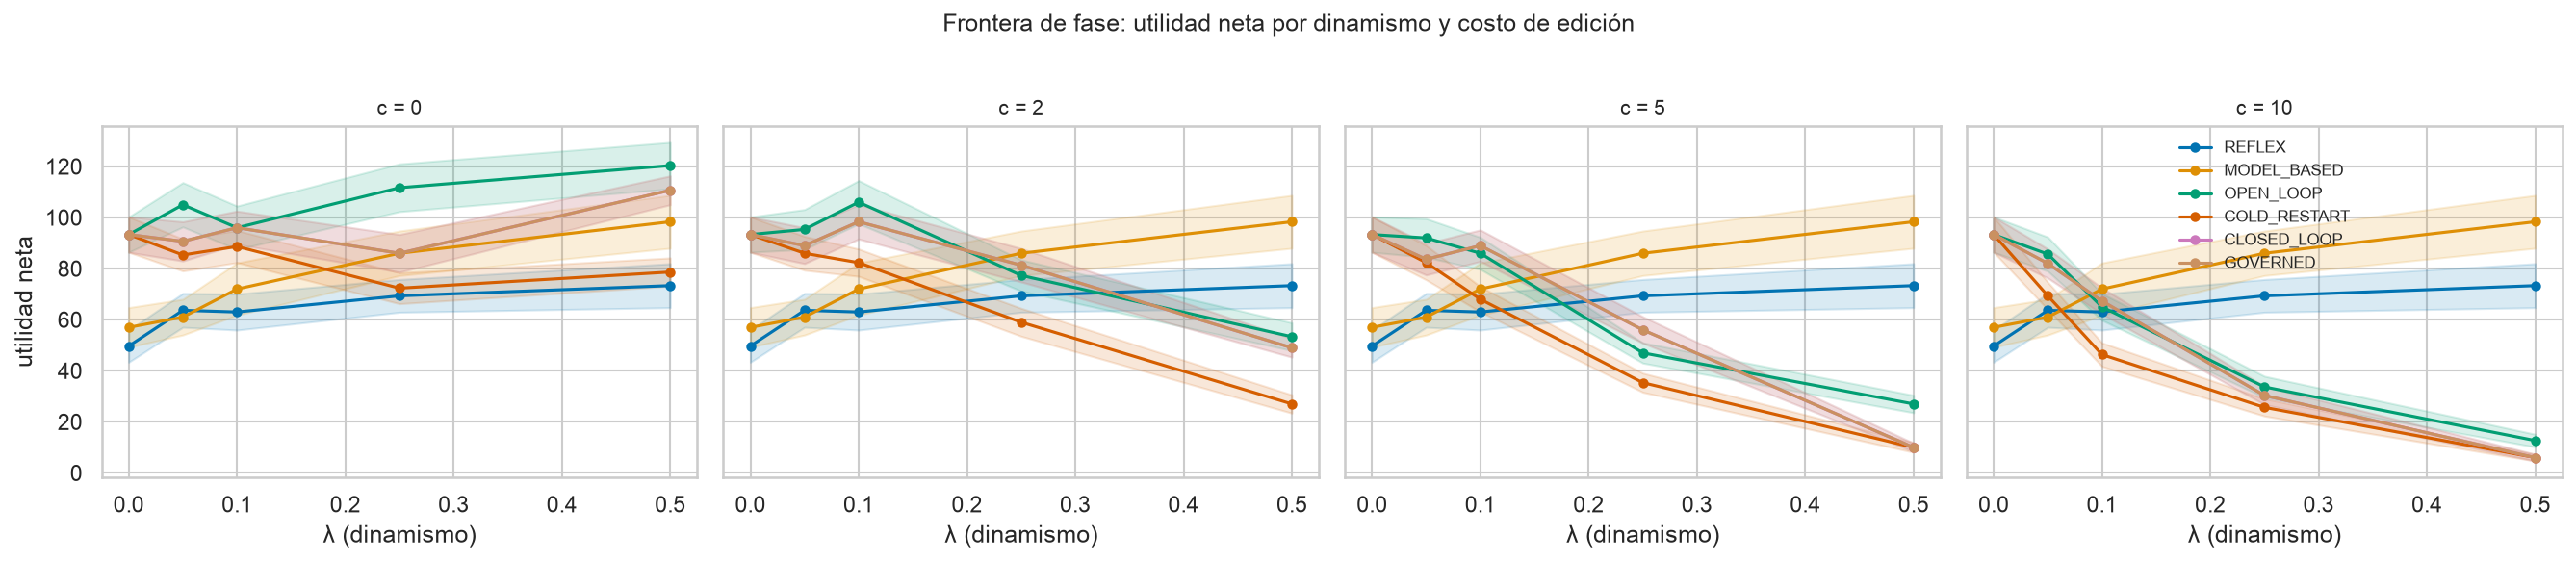
\includegraphics[width=\linewidth]{01-frontera}
  \caption{Frontera de fase: Utilidad neta contra $\lambda$ para las seis arquitecturas originales, un panel por $c$ ($p=0.9$, $r=3$, 3.600 corridas). La banda es el error estándar de la media. \CL{} y \GOV{} se superponen porque este barrido no fija presupuesto, y sin presupuesto \GOV{} es \CL. A medida que crecen $\lambda$ y $c$, las políticas que planifican se hunden mientras que \MB{} (reactiva con creencias, que nunca delibera) mejora con el dinamismo y no depende de $c$.}
  \label{fig:frontera}
\end{figure}

Primeramente, con $\lambda=0$ las cuatro políticas que planifican rinden exactamente lo mismo (93.3, que es el control 1) y casi duplican a las reactivas (49.7 el reflejo simple y 57.0 el basado en modelo), dado que sin dinamismo el plan nunca caduca y la previsión de A* para rodear obstáculos y encadenar objetivos vale más que cualquier reacción.

Progresivamente, a medida que crece $\lambda$, la comparación que motivaba el trabajo (reparar al ver la divergencia, \CL, contra esperar a que el plan falle, \OL) resulta mucho más pareja de lo esperado, pues la diferencia \OL$-$\CL{} va de $-9.0$ a $+25.7$ puntos según la celda y en 13 de las 16 celdas con $\lambda>0$ cae dentro de dos errores estándar. Las únicas celdas en que el lazo abierto se adelanta claramente son $\lambda=0.25$ con $c=0$ (111.7 contra 86.0) y $\lambda=0.5$ con $c=5$ (27.0 contra 10.0) y con $c=10$ (12.7 contra 6.0), y estas dos últimas están en un régimen donde todas las políticas que planifican ya colapsaron, mientras que en ninguna celda el lazo cerrado se adelanta más allá del ruido. Es decir que, con $r=3$ y cuando ambas cosas cuestan lo mismo, monitorear el plan no compra casi nada sobre replanificar solo al fallar.

Finalmente, lo que sí aparece con nitidez es otra frontera, la que separa deliberar de no deliberar en absoluto: El costo $c$ hunde a las políticas que planifican a medida que crece, y el hundimiento se acelera con $\lambda$, mientras que \MB{} no depende de $c$ y mejora con el dinamismo, de forma que pasa a ser la mejor política a $\lambda=0.5$ con cualquier $c\ge2$ (98.3 contra 53.3, 27.0 y 12.7 de la mejor que planifica con $c=2$, 5 y 10) y a $\lambda=0.25$ con $c\ge5$ (86.0 contra 56.0 y 33.7), con márgenes de entre tres y ocho errores estándar; con $c=2$ a $\lambda=0.25$ y con $c=10$ a $\lambda=0.1$ la diferencia cae dentro del ruido. Esa es la frontera que buscaba la pregunta, aunque no entre las dos políticas que se esperaba, pues el costo de reescritura a partir del cual la ventaja se invierte es el costo a partir del cual deja de convenir planificar, y no el que separa al lazo cerrado del abierto.

\begin{table}[htbp]
\centering
\footnotesize
\setlength{\tabcolsep}{4pt}
\begin{tabular}{@{}l rrrr c rrrr@{}}
\toprule
& \multicolumn{4}{c}{\OL{} $-$ \CL} & & \multicolumn{4}{c}{\MB{} $-$ mejor política con plan} \\
\cmidrule{2-5}\cmidrule{7-10}
$\lambda$ & $c=0$ & $c=2$ & $c=5$ & $c=10$ & & $c=0$ & $c=2$ & $c=5$ & $c=10$ \\
\midrule
0    & 0.0 & 0.0 & 0.0 & 0.0 & & \multicolumn{4}{c}{\textbf{−36.3 ± 9.6} (igual en todo $c$)} \\ \sepfilas
0.05 & +14.3 ± 8.2 & +6.3 ± 6.2 & +8.3 ± 6.7 & +3.7 ± 4.4 & & \textbf{−44.0 ± 8.1} & \textbf{−34.3 ± 7.2} & \textbf{−31.0 ± 7.0} & \textbf{−24.7 ± 6.8} \\ \sepfilas
0.1  & 0.0 ± 7.7 & +7.7 ± 8.2 & −3.0 ± 5.9 & −2.3 ± 4.8 & & \textbf{−24.0 ± 11.4} & \textbf{−34.0 ± 9.9} & −17.0 ± 8.8 & +4.7 ± 8.8 \\ \sepfilas
0.25 & \textbf{+25.7 ± 9.0} & −4.0 ± 6.7 & −9.0 ± 5.7 & +3.3 ± 5.7 & & \textbf{−25.7 ± 11.3} & +4.7 ± 9.4 & \textbf{+30.0 ± 10.1} & \textbf{+52.3 ± 9.2} \\ \sepfilas
0.5  & +9.7 ± 9.7 & +4.3 ± 5.3 & \textbf{+17.0 ± 3.8} & \textbf{+6.7 ± 3.1} & & −22.0 ± 11.2 & \textbf{+45.0 ± 11.7} & \textbf{+71.3 ± 9.6} & \textbf{+85.7 ± 10.5} \\
\bottomrule
\end{tabular}
\caption{Las dos diferencias que deciden la frontera (barrido \texttt{principal}). A la izquierda, lazo abierto menos lazo cerrado, casi siempre dentro del ruido. A la derecha, el agente que no delibera menos la política con plan de mayor media en cada celda, que pasa de perder por más de 20 puntos a ganar por más de 45 cuando $\lambda$ y $c$ crecen.}
\label{tab:frontera}
\end{table}

El mecanismo se lee en las métricas de las mismas corridas: A $\lambda=0.5$ con $c=5$, \CL{} pasa en promedio 282 de los 400 ticks deliberando y entrega 1.0 recurso, mientras que \OL, que replanifica menos veces, pasa 154 ticks deliberando y entrega 2.7, de forma que ambos gastan buena parte del horizonte pensando sobre un mundo que se mueve mientras piensan, y cada plan nace desactualizado, en tanto que el agente reactivo reevalúa en cada tick sin detenerse. De ahí se sigue además un matiz sobre la taxonomía de \textcite{russellNorvig2020}, pues su orden depende del entorno de tarea: \RX{} es el peor con $\lambda=0$, pero mejora con el dinamismo y a $\lambda=0.5$ con $c\ge2$ supera también a todo lo que planifica (73.3), de forma que planificar compra previsión y vende oportunismo, y cuál de las dos vale más es una propiedad del entorno y no del agente.

\textbf{Veredicto.} La hipótesis O1 se cumple solo en su parte trivial (con $\lambda=0$ las políticas que planifican empatan), pues con $r=3$ no aparece un umbral $\lambda^{*}$ a partir del cual reparar al ver la divergencia supere a esperar el fallo; la O2 se cumple en otro sentido del previsto, ya que $c$ resultó decisivo, pero para desplazar el punto desde el cual deja de convenir planificar.

\FloatBarrier
\subsection{Cuánto vale reparar en caliente frente a reiniciar en frío}\label{sec:res-caliente}

\CR{} modela a los sistemas que aplican las ediciones en la ejecución siguiente, en los que el trabajo en curso (la carga que el agente ya llevaba) se pierde, mientras que \CL{} repara el plan en caliente y conserva el progreso. Su diferencia es el argumento cuantitativo para decidir si un motor de ejecución agéntica debe reparar en caliente (figura~\ref{fig:caliente} y cuadro~\ref{tab:caliente}).

\begin{figure}[htbp]
  \centering
  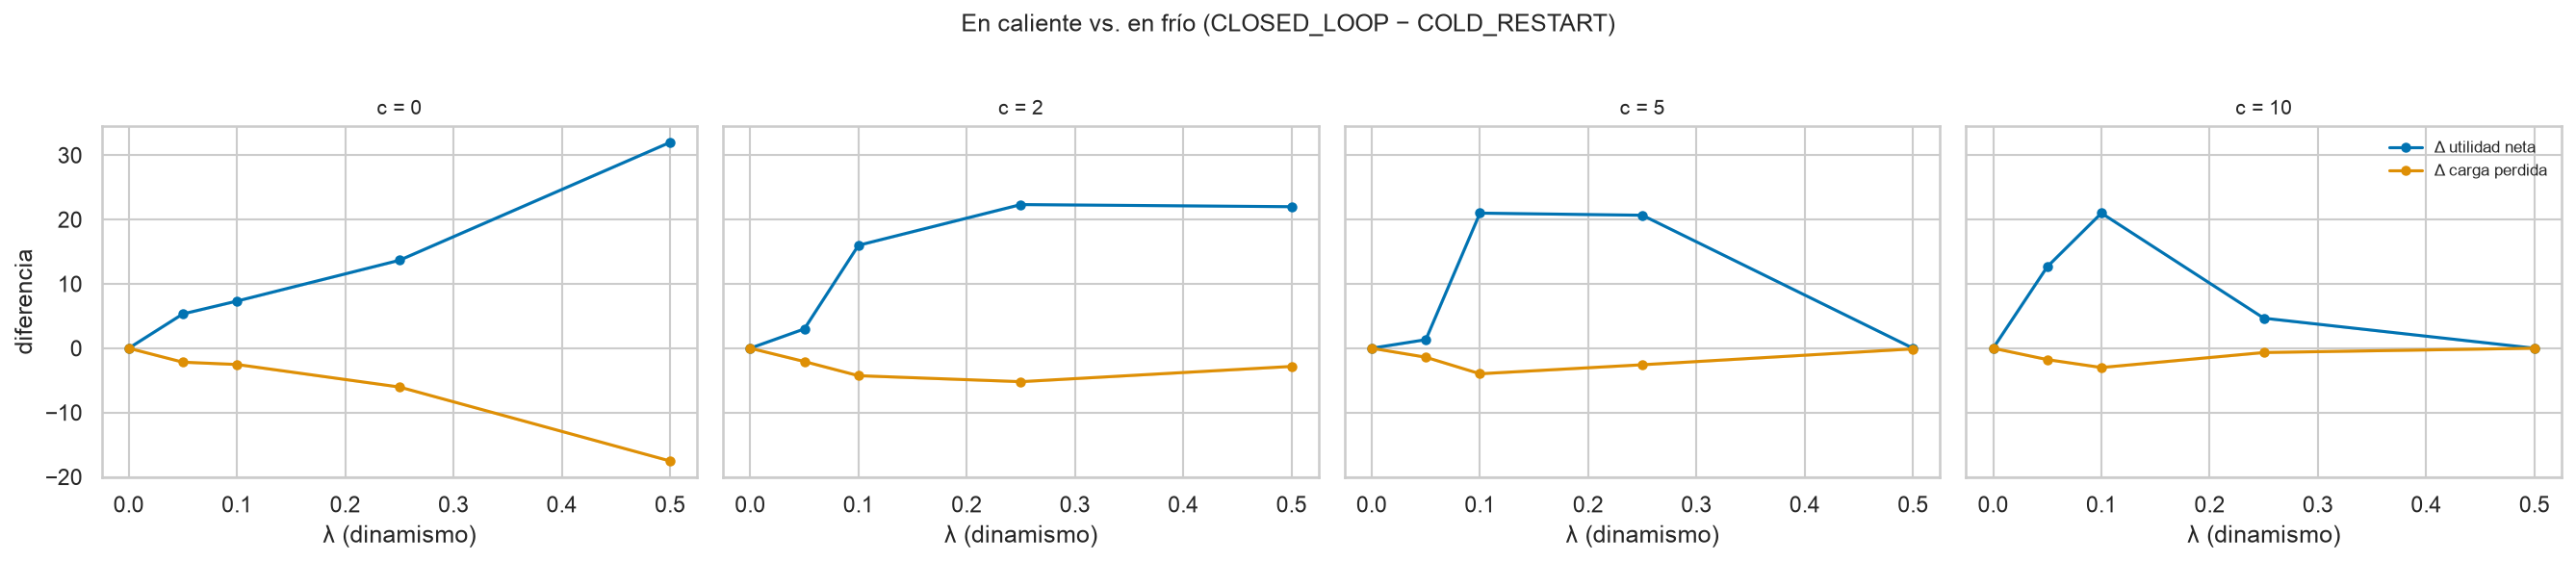
\includegraphics[width=\linewidth]{02-hot-vs-cold}
  \caption{Reparar en caliente menos reiniciar en frío (\CL$-$\CR), un panel por $c$: En azul la diferencia de utilidad neta y en naranja la de carga perdida por corrida. La ventaja es nula en un entorno estático, aparece con claridad desde $\lambda=0.1$ y se anula a $\lambda=0.5$ con $c\ge5$, donde las dos políticas colapsan.}
  \label{fig:caliente}
\end{figure}

\begin{table}[htbp]
\centering
\footnotesize
\begin{tabular}{@{}l rrrr@{}}
\toprule
$\lambda$ & $c=0$ & $c=2$ & $c=5$ & $c=10$ \\
\midrule
0.05 & +5.3 ± 5.0 & +3.0 ± 3.6 & +1.3 ± 5.1 & \textbf{+12.7 ± 4.3} \\ \sepfilas
0.1  & \textbf{+7.3 ± 3.1} & \textbf{+16.0 ± 5.6} & \textbf{+21.0 ± 5.3} & \textbf{+21.0 ± 5.7} \\ \sepfilas
0.25 & \textbf{+13.7 ± 4.2} & \textbf{+22.3 ± 4.1} & \textbf{+20.7 ± 5.6} & \textbf{+4.7 ± 2.1} \\ \sepfilas
0.5  & \textbf{+32.0 ± 5.7} & \textbf{+22.0 ± 4.1} & 0.0 ± 0.8 & 0.0 ± 0.0 \\
\bottomrule
\end{tabular}
\caption{Valor de reparar en caliente: \CL{} $-$ \CR{} en el barrido \texttt{principal} (con $\lambda=0$ la diferencia es exactamente cero).}
\label{tab:caliente}
\end{table}

La ventaja de reparar en caliente es cero en un entorno estático y aparece con claridad desde $\lambda=0.1$, donde vale entre $+7.3$ y $+21.0$ puntos según $c$ (de $+8$\,\% a $+45$\,\%); a $\lambda=0.25$ vale entre $+4.7$ y $+22.3$, y a $\lambda=0.5$ con deliberación gratuita llega a $+32.0$ puntos ($+41$\,\%), sostenida por una caída de 17.5 unidades por corrida en la carga perdida. Con visión total la ventaja es todavía mayor, pues en el barrido de observabilidad el reinicio en frío colapsa y \CL$-$\CR{} llega a \dif{+80.7}{7.0} a $\lambda=0.1$ (145.0 contra 64.3) y a \dif{+47.7}{4.3} a $\lambda=0.25$, que es la ventaja más grande de reparar en caliente en todo el trabajo. Cabe mencionar que esta es la conclusión que mejor sobrevivió a la corrección de la regla de costo, e incluso se fortaleció (a $\lambda=0.1$ con $c=5$ pasó de $+4$ a $+21$ puntos), lo cual tiene sentido, porque ahora las dos políticas pagan lo mismo por cada replanificación y lo único que las separa es el trabajo en curso que una conserva y la otra tira.

Vale la pena matizar dos cosas. Primeramente, la relación con $c$ no es monótona, pues a $\lambda=0.25$ el máximo está en $c=2$ y no en $c=0$, y a $\lambda=0.1$ la ventaja crece con $c$ en vez de caer, de forma que lo defendible es el signo de la ventaja y su aparición desde $\lambda=0.1$, y no el valor de cada celda (el porcentaje, además, se infla cuando el reinicio en frío rinde poco, como el $+81$\,\% de $\lambda=0.5$ con $c=2$, que son 22 puntos sobre una base de 27). Finalmente, la ventaja se anula a $\lambda=0.5$ con $c\ge5$, no porque reiniciar en frío sea bueno ahí, sino porque ambas políticas colapsan (10.0 contra 10.0 con $c=5$), de forma que no queda trabajo en curso que perder.

\textbf{Veredicto.} La hipótesis O5 se confirma: Construir la reparación en caliente compensa en cuanto el entorno cambia con alguna frecuencia (desde $\lambda=0.1$ en este modelo), siempre que deliberar no sea tan caro que el agente deje de completar entregas.

\FloatBarrier
\subsection{La competencia del replanificador}\label{sec:res-competencia}

La competencia $p$ es la probabilidad de que la reparación del oráculo sea la óptima, y su fallo no es ruido sino un plan plausible y equivocado (figura~\ref{fig:competencia}). La competencia sí mueve el resultado, aunque no del modo esperado, pues la política más sensible a $p$ resultó ser el lazo abierto y no el cerrado: Entre $p=0.5$ y $p=1$, \OL{} pasa de 36.7 a 61.0 a $\lambda=0.25$ y de 16.3 a 34.7 a $\lambda=0.5$, mientras que \CL{} pasa de 48.3 a 59.7 a $\lambda=0.25$ y se queda plano a $\lambda=0.5$ (entre 10.0 y 14.0), donde lo que lo hunde es la cantidad de reparaciones que paga y no su calidad; a $\lambda=0.1$ todas las pendientes caen dentro del ruido.

\begin{figure}[htbp]
  \centering
  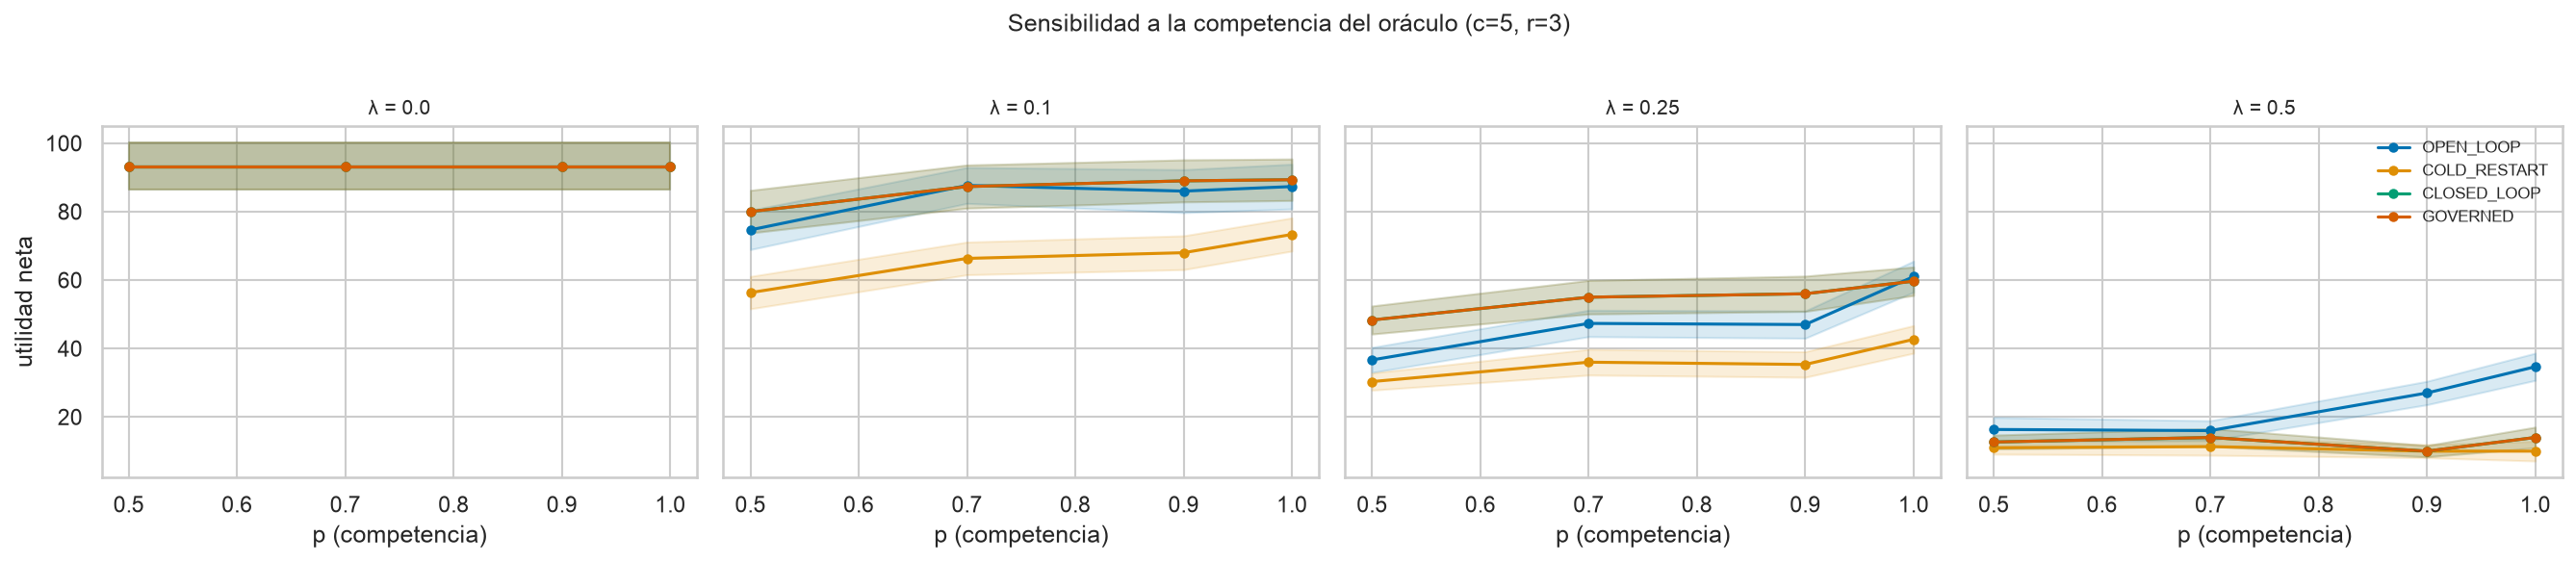
\includegraphics[width=\linewidth]{03-competencia}
  \caption{Sensibilidad a la competencia del oráculo ($c=5$, $r=3$), un panel por $\lambda$. El lazo abierto (azul) es el que más depende de $p$; el cerrado y el gobernado (superpuestos) apenas se mueven, y a $\lambda=0.5$ el abierto se adelanta solo desde $p=0.9$.}
  \label{fig:competencia}
\end{figure}

El orden entre ambas cambia entonces con $p$: Con un replanificador mediocre ($p=0.5$) el lazo cerrado rinde más a $\lambda=0.25$ (\dif{+11.7}{4.7} sobre el abierto), con uno perfecto empatan (59.7 contra 61.0), y a $\lambda=0.5$ el lazo abierto se adelanta solo desde $p=0.9$ (\dif{+17.0}{3.8}, y \dif{+20.7}{4.4} con $p=1$). Una lectura plausible, que no se verificó con una métrica específica, es que un error del replanificador le cuesta al lazo abierto un viaje completo hasta la celda equivocada antes de descubrirlo, mientras que el lazo cerrado lo corrige en la siguiente observación, aunque pagando otra reparación, de forma que la calidad de cada reparación pesa más para quien repara poco. Hay además un límite estructural, pues cuando el agente pide una reparación sin ver su objetivo el oráculo no puede acertar, de modo que con $r=3$ una parte de las consultas no depende de $p$.

\textbf{Veredicto.} La hipótesis O3 no se sostiene: El control 3 pasa solo por el signo y, en el barrido de competencia, un replanificador mediocre favorece incluso al lazo cerrado frente al abierto, de forma que en este barrido no existe una competencia mínima a partir de la cual reparar al ver la divergencia supere a esperar el fallo.

\FloatBarrier
\subsection{Observabilidad parcial}\label{sec:res-observabilidad}

El radio $r$ modela qué parte del entorno tiene el agente en su contexto, y la métrica que importa no es si el agente se entera de una divergencia sino cuándo (figura~\ref{fig:observabilidad} y cuadro~\ref{tab:observabilidad}). La ceguera es casi nula en todos los radios (a lo sumo 3\,\% en promedio por radio y 4.4\,\% en el peor caso, \OL{} con $r=1$), justo como predecía el diseño, pues las divergencias no se pierden sino que se detectan tarde: La latencia promedio baja de 1.24–1.27 ticks con $r=1$ y $r=3$ (entre los cuales no hay un orden claro) a 0.72 con $r=\infty$.

\begin{figure}[htbp]
  \centering
  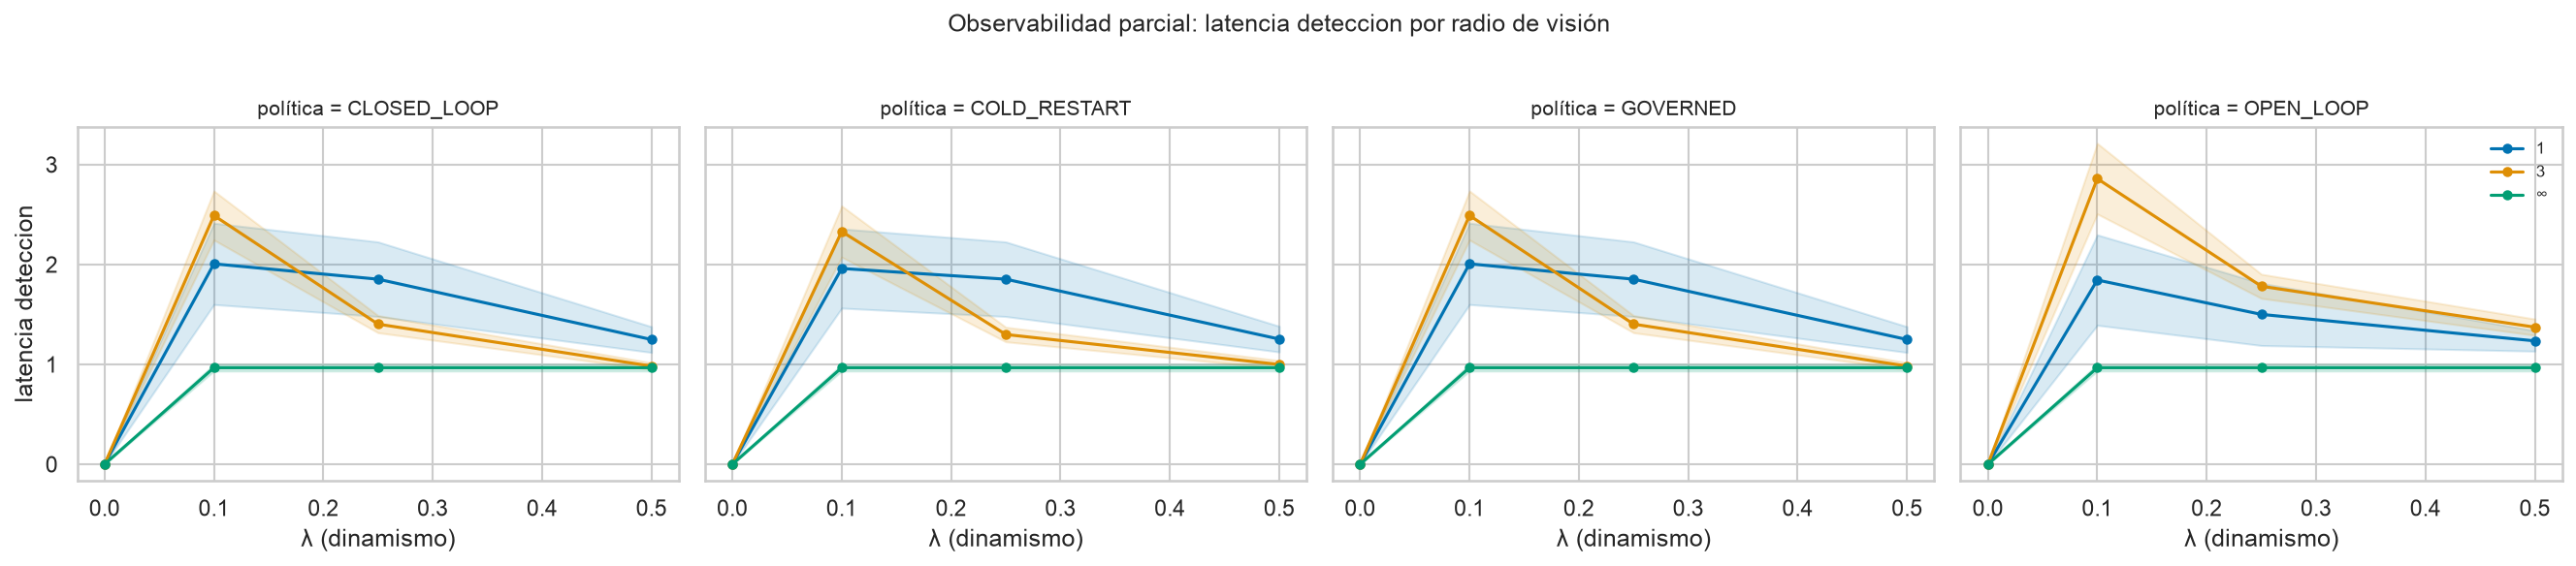
\includegraphics[width=\linewidth]{04-observabilidad}
  \caption{Latencia de detección (ticks entre que ocurre una divergencia y el agente la nota) contra $\lambda$, una línea por radio y un panel por política ($c=5$, $p=0.9$). Con visión total la latencia es la mínima posible; con $r=1$ y $r=3$ el agente camina en promedio uno o dos ticks más hacia una celda donde el recurso ya no está.}
  \label{fig:observabilidad}
\end{figure}

\begin{table}[htbp]
\centering
\footnotesize
\begin{tabular}{@{}l rrrr rrr@{}}
\toprule
$r$ & Latencia & Ceguera & Ediciones & Utilidad & $U(\lambda=0)$ & \OL{} & \CL{} \\
\midrule
1        & 1.24 & 0.03 & 1.46  & 48.1  & 47.0  & 48.0  & 47.9 \\ \sepfilas
3        & 1.27 & 0.02 & 10.95 & 59.8  & 93.3  & 63.3  & 62.1 \\ \sepfilas
$\infty$ & 0.72 & 0.00 & 14.81 & 110.2 & 261.0 & 129.5 & 114.5 \\
\bottomrule
\end{tabular}
\caption{Observabilidad parcial, promedios por radio sobre $\lambda \in \{0, 0.1, 0.25, 0.5\}$ y las cuatro políticas con plan ($c=5$). Las dos últimas columnas son la utilidad media del lazo abierto y del cerrado.}
\label{tab:observabilidad}
\end{table}

La utilidad media sube de 48.1 con $r=1$ a 59.8 con $r=3$ y 110.2 con $r=\infty$, pero la tesis de una versión anterior del modelo (que la observabilidad dominaba todo lo demás y que con visión total la replanificación ganaba) no sobrevivió a la corrección, y la lectura actual tiene tres partes:

\begin{itemize}[leftmargin=1.4em, itemsep=0.2em]
  \item \textbf{La observabilidad fija el nivel de todas las políticas por igual:} Con $\lambda=0$, donde nadie replanifica, las cuatro rinden 47.0 con $r=1$, 93.3 con $r=3$ y 261.0 con $r=\infty$, de forma que buena parte del salto entre radios es que ver más permite encontrar más recursos, lo cual no dice nada sobre si conviene reescribir el plan.
  \item \textbf{Con $r=1$ las políticas son indistinguibles:} En todo $\lambda$ quedan a menos de 4 puntos entre sí, con un error estándar de ese mismo orden, dado que con tan poca visión el agente apenas edita su plan (entre 1.0 y 2.6 ediciones por corrida).
  \item \textbf{Con visión total las diferencias se amplían, pero no a favor de reparar al ver la divergencia:} El lazo abierto supera al cerrado a $\lambda=0.25$ (72.0 contra 52.0, \dif{+20.0}{5.1}) y a $\lambda=0.5$ (34.0 contra 0.0, \dif{+34.0}{4.5}), porque viéndolo todo el lazo cerrado detecta cada divergencia en cuanto ocurre y paga $c$ por cada una, de forma que a $\lambda=0.5$ pasa 372 de los 400 ticks deliberando y no completa ninguna entrega, mientras que el abierto delibera 171 ticks y entrega 3.4 recursos.
\end{itemize}

Es decir que la observabilidad amplifica lo que el costo de deliberar decide: Con deliberación gratuita y oráculo perfecto (el control 2, que también es con $r=\infty$) el lazo cerrado sí domina, por $+45$ y $+56$ puntos a $\lambda=0.25$ y $0.5$, mientras que con $c=5$ y $p=0.9$ pierde en esos mismos $\lambda$. Vale la pena anotar con honestidad que entre esos dos puntos cambian a la vez $c$ y $p$, por lo que la inversión no se puede atribuir solo al costo (aunque §\ref{sec:res-competencia} sugiere que $p$ pesa poco sobre el lazo cerrado), y que el barrido de observabilidad solo tiene $c=5$.

\FloatBarrier
\subsection{Gobernanza: acotar las reparaciones}\label{sec:res-gobernanza}

\GOV{} es reparación en caliente con un presupuesto de $B$ reparaciones proactivas, de forma que agotado el presupuesto se comporta exactamente como el lazo abierto, y el barrido va desde $B=0$ (el lazo abierto, control 6) hasta $B=25$, que en la práctica coincide con \CL{} (figura~\ref{fig:gobernanza} y cuadro~\ref{tab:gobernanza}).

\begin{figure}[htbp]
  \centering
  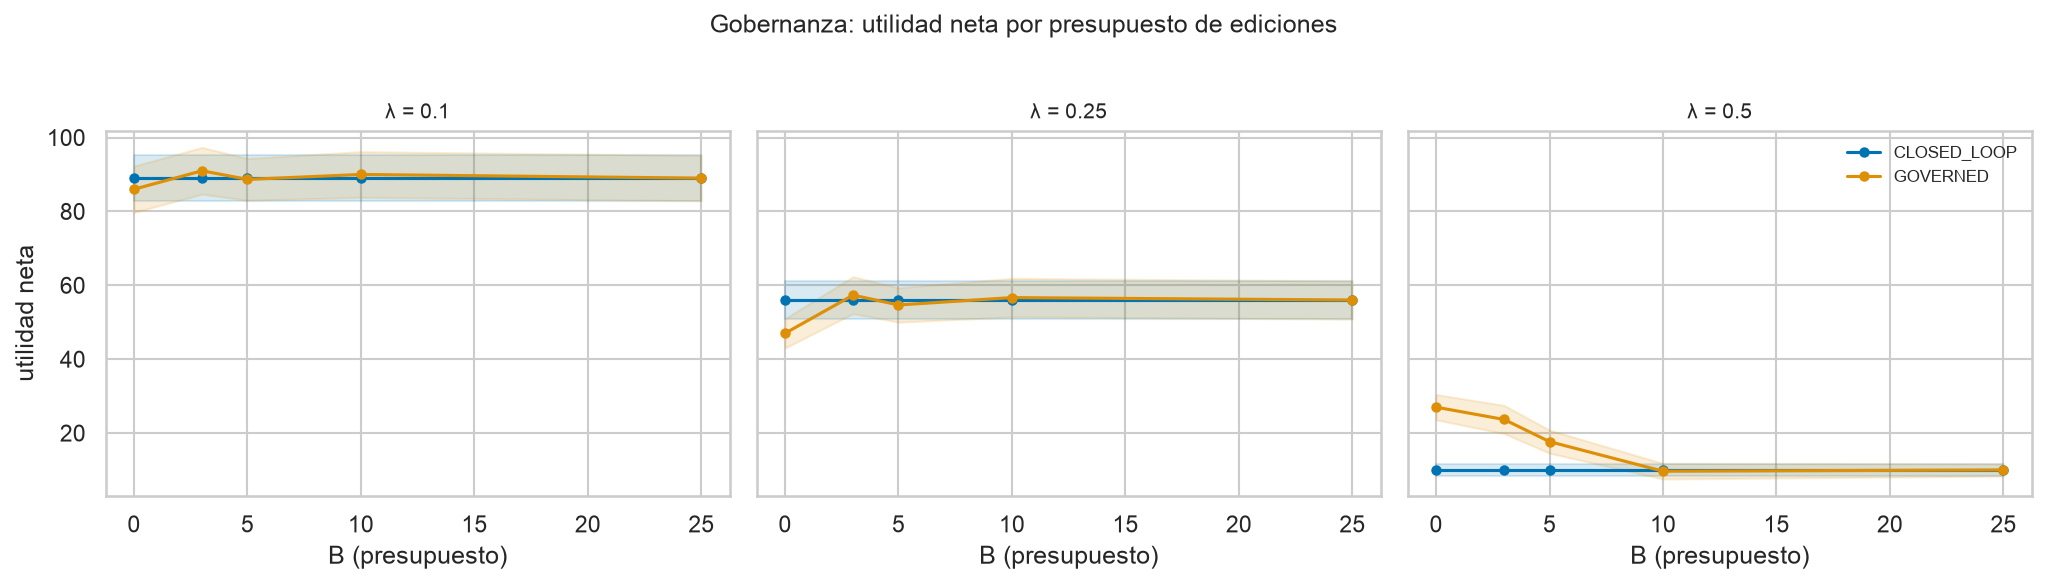
\includegraphics[width=\linewidth]{05-gobernanza}
  \caption{Utilidad neta contra el presupuesto $B$ de reparaciones proactivas, un panel por $\lambda$ ($c=5$, $r=3$). \CL{} no tiene presupuesto y aparece como referencia horizontal; $B=0$ es exactamente \OL. Solo a $\lambda=0.5$ el presupuesto separa a \GOV{} del lazo cerrado, y ahí el mejor presupuesto es cero.}
  \label{fig:gobernanza}
\end{figure}

\begin{table}[htbp]
\centering
\footnotesize
\begin{tabular}{@{}l rrr rrr@{}}
\toprule
& \multicolumn{3}{c}{Utilidad neta} & \multicolumn{3}{c}{Mecanismo a $\lambda=0.5$} \\
\cmidrule(lr){2-4}\cmidrule(l){5-7}
& $\lambda=0.1$ & $\lambda=0.25$ & $\lambda=0.5$ & Desperdiciadas & Ticks deliberando & Por fallo \\
\midrule
\GOV, $B=0$ ($\equiv$ \OL) & 86.0 & 47.0 & 27.0 & 10.1  & 153.6 & 30.6 \\ \sepfilas
\GOV, $B=3$  & 91.0 & 57.3 & 23.7 & 50.7  & 187.7 & 22.4 \\ \sepfilas
\GOV, $B=5$  & 88.7 & 54.7 & 17.7 & 75.3  & 206.7 & 18.9 \\ \sepfilas
\GOV, $B=10$ & 90.0 & 56.7 & 9.7  & 129.0 & 248.6 & 10.4 \\ \sepfilas
\GOV, $B=25$ & 89.0 & 56.0 & 10.0 & 181.1 & 282.0 & 1.2 \\ \sepfilas
\CL          & 89.0 & 56.0 & 10.0 & 181.8 & 282.2 & 1.1 \\
\bottomrule
\end{tabular}
\caption{Gobernanza por presupuesto (medias por corrida, $c=5$, $r=3$). Las tres últimas columnas son, a $\lambda=0.5$, las ediciones desperdiciadas, los ticks deliberando y las replanificaciones forzadas por un fallo.}
\label{tab:gobernanza}
\end{table}

El presupuesto no rescata al lazo cerrado del modo en que parecía en la versión anterior del modelo, cuyo «rescate» era en su mayor parte el mismo artefacto de la replanificación gratuita. A $\lambda=0.1$ el presupuesto no mueve nada medible (todas las variantes quedan entre 86.0 y 91.0, con un error estándar de unos 6 puntos); a $\lambda=0.25$ un presupuesto pequeño recupera el nivel del lazo cerrado (57.3 con $B=3$ contra 56.0), y lo que rinde menos es no reparar nunca de forma proactiva (47.0 con $B=0$), aunque esa diferencia de unos 10 puntos apenas supera dos errores estándar; y a $\lambda=0.5$ acotar sí ayuda frente al lazo cerrado sin acotar (23.7 con $B=3$ contra 10.0), pero la utilidad decrece con $B$ y el mejor presupuesto es cero (27.0, aunque su diferencia con $B=3$ cae dentro del ruido), de forma que lo que mejora el rendimiento no es una cuota óptima sino reparar menos, y todo el régimen queda muy por debajo del 98.3 de \MB.

El mecanismo confirma que el \emph{thrashing} es real y que el presupuesto lo corta, pues a $\lambda=0.5$ las ediciones desperdiciadas caen de 181.8 por corrida en el lazo cerrado a 50.7 con $B=3$ y a 10.1 con $B=0$, y los ticks deliberando de 282 a 188 y 154. Cabe mencionar que acotar las reparaciones proactivas no elimina las replanificaciones sino que las desplaza hacia las forzadas por un fallo (de 1.1 por corrida a 22.4 con $B=3$ y 30.6 con $B=0$), que también se pagan.

\textbf{Veredicto.} La hipótesis O4 se cumple solo en parte: Acotar evita el peor caso cuando el entorno cambia rápido y deliberar es caro, pero no hay una cuota óptima que rescate al agente, y el presupuesto explica a lo sumo el 0.3\,\% de la varianza de la utilidad (§\ref{sec:res-sensibilidad}).

\FloatBarrier
\subsection{Robustez al orden de activación}\label{sec:res-orden}

Por defecto el recolector actúa en cada tick antes de que los recursos deriven, lo cual fija a mano la sincronización de las divergencias, y como la sesión de predador–presa del curso advierte, quien mueve primero gana o pierde información de forma sistemática, de modo que es una amenaza de validez interna. El barrido \texttt{orden} repite un subconjunto de \texttt{principal} sorteando el orden en cada tick, y lo que se compara es el signo de las tres diferencias que sostienen las conclusiones (cuadro~\ref{tab:orden}).

\begin{table}[htbp]
\centering
\footnotesize
\setlength{\tabcolsep}{4pt}
\begin{tabular}{@{}ll rr rr rr@{}}
\toprule
& & \multicolumn{2}{c}{Caliente $-$ frío} & \multicolumn{2}{c}{Abierto $-$ cerrado} & \multicolumn{2}{c}{\ab{MB} $-$ mejor con plan} \\
\cmidrule(lr){3-4}\cmidrule(lr){5-6}\cmidrule(l){7-8}
$\lambda$ & $c$ & Fijo & Sorteado & Fijo & Sorteado & Fijo & Sorteado \\
\midrule
0.1  & 2 & \textbf{+16.0 ± 5.6} & \textbf{+9.3 ± 3.3} & +7.7 ± 8.2 & +8.7 ± 4.6 & −34.0 & −27.7 \\ \sepfilas
0.1  & 5 & \textbf{+21.0 ± 5.3} & \textbf{+9.7 ± 3.9} & −3.0 ± 5.9 & \textbf{+13.3 ± 5.1} & −17.0 & −22.7 \\ \sepfilas
0.25 & 2 & \textbf{+22.3 ± 4.1} & \textbf{+15.3 ± 5.0} & −4.0 ± 6.7 & \textbf{+12.3 ± 5.1} & +4.7 & −12.0 \\ \sepfilas
0.25 & 5 & \textbf{+20.7 ± 5.6} & \textbf{+16.0 ± 3.6} & −9.0 ± 5.7 & +5.3 ± 6.2 & +30.0 & +16.3 \\ \sepfilas
0.5  & 2 & \textbf{+22.0 ± 4.1} & \textbf{+26.7 ± 4.4} & +4.3 ± 5.3 & +3.7 ± 5.0 & +45.0 & +33.7 \\ \sepfilas
0.5  & 5 & 0.0 ± 0.8 & \textbf{+3.3 ± 1.2} & \textbf{+17.0 ± 3.8} & \textbf{+14.0 ± 5.2} & +71.3 & +57.7 \\
\bottomrule
\end{tabular}
\caption{Las tres diferencias que sostienen las conclusiones, con el orden de activación fijo (\texttt{principal}) y sorteado (\texttt{orden}), con $r=3$ y $p=0.9$. La última columna compara medias, sin error estándar.}
\label{tab:orden}
\end{table}

Las dos conclusiones cualitativas que sostienen el trabajo no dependen de quién mueve primero. Primeramente, en la comparación entre caliente y frío el signo coincide en 5 de las 6 celdas, y la sexta no es una excepción real, pues con orden fijo a $\lambda=0.5$ y $c=5$ las dos políticas colapsan y empatan, mientras que con orden sorteado la ventaja del caliente es pequeña pero positiva; con orden sorteado la ventaja es positiva en las seis celdas, aunque más chica que con orden fijo a $\lambda=0.1$ (+9.3 y +9.7 contra +16.0 y +21.0), lo cual deja la conclusión intacta en signo y la vuelve prudente en magnitud. Progresivamente, en la comparación entre no planificar y planificar el signo coincide también en 5 de 6 celdas, y la que cambia ($\lambda=0.25$ con $c=2$) es justamente la que el barrido principal ya había dejado dentro del ruido, mientras que donde \MB{} ganaba sigue ganando, por entre $+16.3$ y $+57.7$ puntos. Finalmente, la diferencia entre lazo abierto y cerrado cambia de signo en 3 de 6 celdas, que es lo que cabe esperar de una diferencia que ya estaba dentro de dos errores estándar en casi todo el rango; vale la pena anotar que con orden sorteado el lazo abierto queda arriba en las seis celdas, y en tres de ellas por más de dos errores estándar, de modo que si el orden mueve algo es a favor de no monitorear.

\textbf{Veredicto.} La hipótesis se confirma para las dos conclusiones cualitativas (reparar en caliente supera al frío con $\lambda>0$, y no planificar gana con $\lambda$ alto y deliberación cara), mientras que la comparación entre lazo abierto y lazo cerrado, que ya era la más frágil, no tiene un signo estable.

\FloatBarrier
\subsection{Dinámica: cuándo se separan las políticas}\label{sec:res-dinamica}

Los barridos guardan solo el valor final de cada corrida, de modo que no dicen \emph{cuándo} se separan las políticas. Las series temporales repiten la rebanada central de la frontera ($c=5$, $r=3$, $p=0.9$) con cinco políticas, cuatro valores de $\lambda$ y 30 semillas, guardando una fila cada cinco ticks. El plan de esta extensión suponía que las políticas se separan en un momento identificable, por ejemplo cuando se acumulan las primeras divergencias, y lo que se encontró es otra cosa (cuadros~\ref{tab:dinamica} y~\ref{tab:separacion}).

\begin{table}[htbp]
\centering
\footnotesize
\begin{tabular}{@{}l ccccc@{}}
\toprule
$\lambda$ & \RX & \MB & \OL & \CR & \CL \\
\midrule
0    & 1.8 / 3.2 / 5.0 & 1.7 / 3.7 / 5.7 & 2.7 / 5.0 / 9.3 & 2.7 / 5.0 / 9.3 & 2.7 / 5.0 / 9.3 \\ \sepfilas
0.1  & 2.5 / 3.9 / 6.3 & 2.6 / 4.4 / 7.2 & 2.3 / 4.5 / 8.6 & 2.2 / 4.0 / 6.8 & 2.4 / 4.6 / 8.9 \\ \sepfilas
0.25 & 2.9 / 4.4 / 6.9 & 3.3 / 5.3 / 8.6 & 1.4 / 2.4 / 4.7 & 1.3 / 1.9 / 3.5 & 1.6 / 3.0 / 5.6 \\ \sepfilas
0.5  & 2.7 / 4.9 / 7.3 & 3.2 / 5.8 / 9.8 & 0.6 / 1.3 / 2.7 & 0.3 / 0.6 / 1.0 & 0.3 / 0.6 / 1.0 \\
\bottomrule
\end{tabular}
\caption{Entregas acumuladas medias en los ticks 100, 200 y 400 ($c=5$, $r=3$, 600 corridas). El crecimiento es casi lineal en todas las celdas.}
\label{tab:dinamica}
\end{table}

\begin{table}[htbp]
\centering
\footnotesize
\begin{tabular}{@{}l llll@{}}
\toprule
$\lambda$ & \ab{MB}$-$\ab{CL} & \ab{MB}$-$\ab{OL} & \ab{CL}$-$\ab{CR} & \ab{OL}$-$\ab{CL} \\
\midrule
0    & tick 50 (−3.6 ± 1.0) & tick 50 (−3.6 ± 1.0) & nunca (0.0) & nunca (0.0) \\ \sepfilas
0.1  & nunca (−1.7 ± 0.9) & nunca (−1.4 ± 1.1) & tick 130 (+2.1 ± 0.5) & nunca (−0.3 ± 0.6) \\ \sepfilas
0.25 & tick 30 (+3.0 ± 1.0) & tick 25 (+3.9 ± 0.9) & tick 105 (+2.1 ± 0.6) & nunca (−0.9 ± 0.6) \\ \sepfilas
0.5  & tick 15 (+8.8 ± 1.0) & tick 15 (+7.1 ± 1.0) & nunca (+0.0 ± 0.1) & tick 170 (+1.7 ± 0.4) \\
\bottomrule
\end{tabular}
\caption{Primer tick desde el cual la diferencia pareada de entregas supera dos errores estándar y ya no vuelve a bajar hasta el final; entre paréntesis, la diferencia en entregas en el tick 400.}
\label{tab:separacion}
\end{table}

La separación no es un evento sino un ritmo. Las curvas de entregas acumuladas son casi rectas desde el tick 50, de forma que cada política entrega a un paso que fija $\lambda$ y lo mantiene (\CL{} a $\lambda=0.1$ entrega 2.1 recursos por cada 100 ticks tanto entre los ticks 50 y 200 como entre los 200 y 400, y \OL{} a $\lambda=0.5$, 0.7 en ambos tramos), por lo que las diferencias finales de la frontera son pendientes distintas acumuladas durante 400 ticks y no el resultado de un episodio puntual. Con $\lambda$ alto, no planificar se adelanta casi de inmediato (\MB{} supera al lazo cerrado desde el tick 15 con $\lambda=0.5$ y desde el 30 con $\lambda=0.25$), lo cual es la frontera de §\ref{sec:res-frontera} vista en el tiempo; reparar en caliente, en cambio, tarda en pagar, pues su ventaja sobre el frío se separa del ruido recién desde el tick 130 con $\lambda=0.1$ y el 105 con $\lambda=0.25$, cuando el agente ya acumuló trabajo en curso que un reinicio tiraría. Los ticks deliberando también crecen en línea recta (a $\lambda=0.5$, \CL{} delibera 64 de los primeros 100 ticks y 282 de los 400), de modo que el \emph{thrashing} no es una crisis que llegue en algún momento sino un impuesto que se cobra desde el principio y a ritmo constante.

\FloatBarrier
\subsection{El agente basado en conocimiento}\label{sec:res-kb}

La figura~\ref{fig:conocimiento} reúne las cinco políticas del barrido \texttt{conocimiento}, una faceta por radio, y el cuadro~\ref{tab:kb} pone en números los contrastes de H1, de la ablación, de H1b y de H3. Primero los controles exactos (cuadro~\ref{tab:controles}), que pasan sin una sola corrida distinta: Con visión total y el horizonte \ahora{} la región lógica es exactamente el monitor de \CL{} (H2), y añadir las dos políticas nuevas no tocó a las demás.

\begin{figure}[htbp]
  \centering
  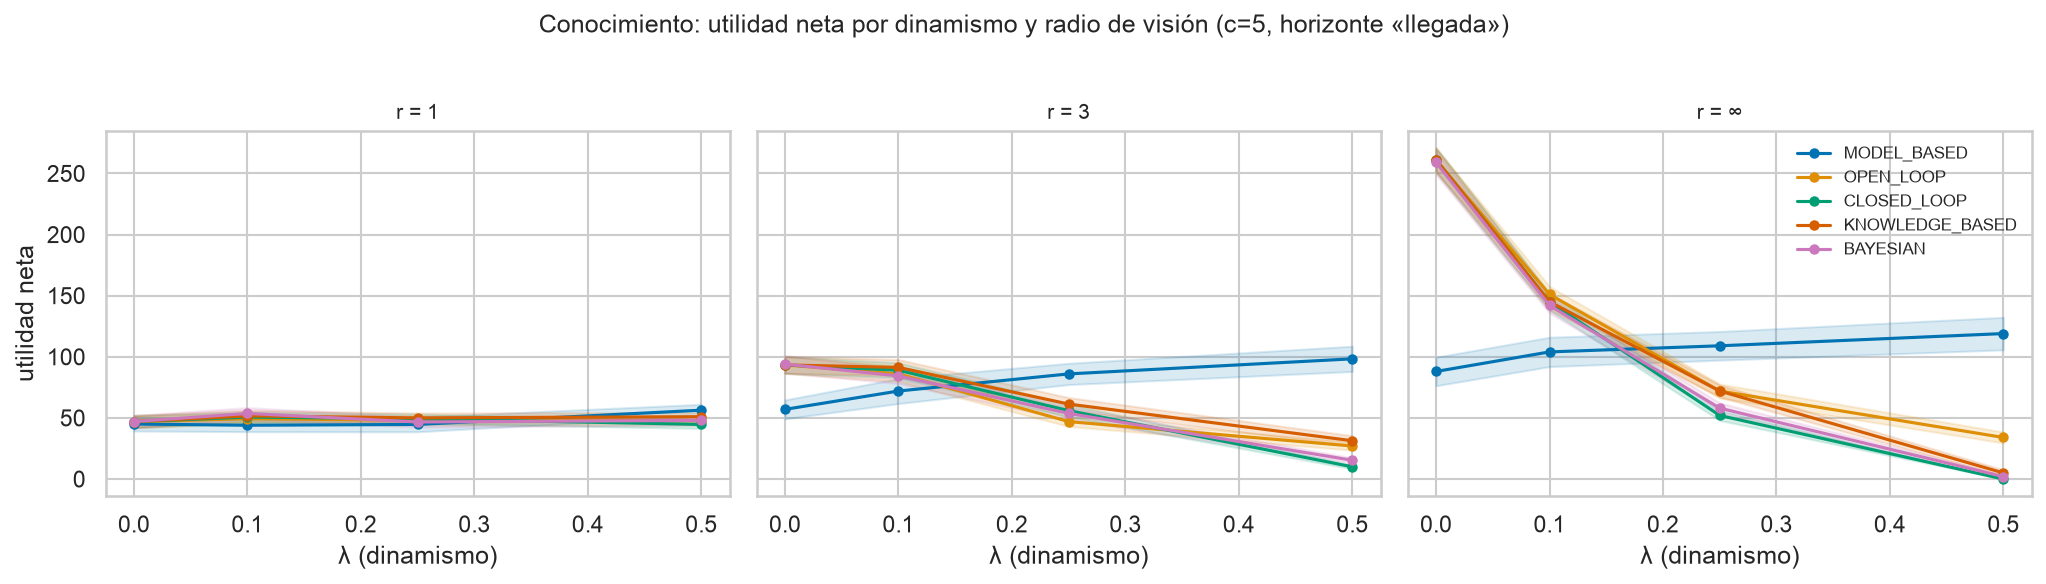
\includegraphics[width=\linewidth]{06-conocimiento}
  \caption{Utilidad neta de las cinco políticas del barrido \texttt{conocimiento} ($c=5$, horizonte \llegada), una faceta por radio. Con $r=1$ todas quedan juntas; con $r=3$ \KB{} queda por encima del lazo cerrado a $\lambda=0.5$ pero muy por debajo de \MB; con visión total ninguna política con plan resiste el dinamismo alto.}
  \label{fig:conocimiento}
\end{figure}

\begin{table}[htbp]
\centering
\footnotesize
\setlength{\tabcolsep}{3.5pt}
\begin{tabular}{@{}l rrrr rrr@{}}
\toprule
& \multicolumn{4}{c}{Contrastes ($r=3$, consulta gratuita)} & \multicolumn{3}{c}{H3: \ab{KB}$-$\ab{CL} con costo por consulta} \\
\cmidrule(lr){2-5}\cmidrule(l){6-8}
$\lambda$ & H1: \ab{KB}$-$\ab{CL} & \ab{KB} \ahora{}$-$\ab{CL} & \ab{KB}$-$\ab{OL} & \ab{KB}$-$\ab{MB} & 1 tick & 2 ticks & 5 ticks \\
\midrule
0.1  & +2.3 ± 6.1 & +5.7 ± 4.1 & +5.3 ± 4.7 & +19.3 ± 10.6 & −5.3 ± 5.5 & −9.0 ± 4.8 & \textbf{−32.3 ± 5.6} \\ \sepfilas
0.25 & +5.3 ± 6.2 & −3.0 ± 5.1 & \textbf{+14.3 ± 4.2} & \textbf{−24.7 ± 9.8} & \textbf{−17.3 ± 5.6} & \textbf{−30.3 ± 5.8} & \textbf{−36.7 ± 5.6} \\ \sepfilas
0.5  & \textbf{+21.3 ± 3.8} & −1.3 ± 2.6 & +4.3 ± 5.3 & \textbf{−67.0 ± 10.5} & −2.3 ± 2.0 & −3.7 ± 1.9 & \textbf{−4.7 ± 2.0} \\
\bottomrule
\end{tabular}
\caption{Agente basado en conocimiento con $r=3$ y $c=5$. La segunda columna es la ablación con horizonte \ahora, que conserva la elección de objetivo por peor caso y vuelve la decisión de reparar idéntica al monitor del lazo cerrado.}
\label{tab:kb}
\end{table}

\begin{table}[htbp]
\centering
\footnotesize
\begin{tabular}{@{}ll rrrrrr@{}}
\toprule
$\lambda$ & Política & Por fallo & Proactivas & Desperdiciadas & Ticks deliberando & Consultas & Entregas \\
\midrule
0.1  & \OL & 10.6 & 0.0 & 3.6 & 53.5 & 0.0 & 8.6 \\
     & \CL & 1.6 & 7.7 & 7.1 & 56.2 & 0.0 & 8.9 \\
     & \KB & 7.3 & 2.8 & 4.4 & 53.7 & 16.0 & 9.1 \\
     & \BY & 3.3 & 6.2 & 5.9 & 56.2 & 23.1 & 8.4 \\ \sepfilas
0.25 & \OL & 21.6 & 0.0 & 7.7 & 108.8 & 0.0 & 4.7 \\
     & \CL & 1.6 & 9.7 & 35.5 & 109.9 & 0.0 & 5.6 \\
     & \KB & 9.3 & 6.5 & 24.1 & 115.5 & 58.9 & 6.1 \\
     & \BY & 7.1 & 11.9 & 38.9 & 145.6 & 75.7 & 5.4 \\ \sepfilas
0.5  & \OL & 30.6 & 0.0 & 10.1 & 153.6 & 0.0 & 2.7 \\
     & \CL & 1.1 & 13.7 & 181.8 & 282.2 & 0.0 & 1.0 \\
     & \KB & 6.6 & 9.5 & 97.4 & 219.2 & 192.1 & 3.1 \\
     & \BY & 5.7 & 16.3 & 145.8 & 265.1 & 208.1 & 1.5 \\
\bottomrule
\end{tabular}
\caption{Mecanismo con $r=3$ y $c=5$ (medias por corrida): Replanificaciones forzadas por un fallo, reparaciones proactivas (las disparadas por una divergencia), ediciones desperdiciadas, ticks deliberando, consultas a la KB o al filtro ante una divergencia y entregas.}
\label{tab:mecanismo}
\end{table}

Los veredictos, en el orden de las hipótesis:

\begin{itemize}[leftmargin=1.4em, itemsep=0.2em]
  \item \textbf{H1, a medias:} El signo es el esperado en todas las celdas con $r \in \{1,3\}$ y $\lambda>0$, pero la diferencia solo supera el ruido con $r=3$ y $\lambda=0.5$ (\dif{+21.3}{3.8}, con 31.3 contra 10.0), mientras que con $r=1$ queda entre $+0.7$ y $+6.3$, dentro de dos errores estándar, como era de esperar donde las políticas con plan casi no se separan. Fuera del alcance de H1, con visión total, \KB{} también supera al cerrado a $\lambda=0.25$ (\dif{+20.0}{5.3}).
  \item \textbf{La ablación dice de dónde sale la ganancia:} Con el horizonte \ahora{} la ventaja desaparece (\dif{+5.7}{4.1}, \dif{-3.0}{5.1} y \dif{-1.3}{2.6}), de modo que las preguntas 1 y 2 por sí solas, que son las que atacan la creencia obsoleta, no compran nada medible, y todo lo que gana \KB{} viene de la pregunta 3 con horizonte \llegada, es decir, de no pagar reparaciones ante derivas de las que el recurso todavía puede volver.
  \item \textbf{H1b, solo con dinamismo bajo:} A $\lambda=0.1$ alcanza a la mejor política sin reparación proactiva (\dif{+5.3}{4.7} sobre \OL), pero desde $\lambda=0.25$ queda por debajo de \MB{} (\dif{-24.7}{9.8} y \dif{-67.0}{10.5}), tal como se había anticipado para $\lambda=0.5$, de forma que saber más no compensa frente a no planificar cuando el mundo cambia rápido.
  \item \textbf{H3, confirmada con fuerza:} Con un solo tick por consulta el signo de la ventaja se invierte en las tres celdas (aunque solo fuera del ruido a $\lambda=0.25$), y con cinco ticks la pérdida llega a $-32.3$ y $-36.7$ a $\lambda=0.1$ y $0.25$, mientras que a $\lambda=0.5$ es solo $-4.7$, porque ahí las políticas con plan ya están cerca del colapso. La frontera análoga a la de $c$ existe y está muy cerca de cero, de forma que razonar solo compensa si es casi gratis frente a deliberar.
  \item \textbf{H4, confirmada:} El horizonte \llegada{} multiplica las replanificaciones forzadas por un fallo (7.3, 9.3 y 6.6 por corrida contra 1.6, 1.6 y 1.1 del cerrado) y recorta las proactivas (2.8, 6.5 y 9.5 contra 7.7, 9.7 y 13.7), y a $\lambda=0.5$ delibera \dif{63.0}{13.6} ticks menos y desperdicia 97.4 ediciones contra 181.8, mientras que con $\lambda\le0.25$ los ticks deliberando no cambian más allá del ruido. El intercambio de reparaciones por fallos solo deja ganancia neta donde hay mucho \emph{thrashing} que cortar.
\end{itemize}

Vale la pena anotar un límite que la figura deja a la vista: Con visión total y $\lambda=0.5$, \KB{} se queda en 5.0 frente a 34.0 del lazo abierto, con 211.5 ediciones desperdiciadas por corrida (contra 313.6 del cerrado y 10.0 del abierto), de modo que cuando el agente lo ve todo el horizonte lógico no basta para cortar el \emph{thrashing}.

La figura~\ref{fig:tira-kb} muestra la región posible en acción, en una corrida con $\lambda=0.25$. La región se comporta como dicen los axiomas: En el tick 12 es una mancha pequeña alrededor de la última celda vista, en los ticks 20 y 40 ya cubre buena parte del mapa (con $\lambda=0.25$, una observación de hace veinte ticks apenas descarta nada), y en el tick 64 se encoge de nuevo, porque el disco de visión resta las celdas que ve vacías y colapsa a un punto la región de cada recurso que vuelve a ver. La flecha roja del tick 20 es una divergencia que el agente detecta y \emph{no} repara, porque el recurso todavía puede estar en su celda cuando llegue.

\begin{figure}[htbp]
  \centering
  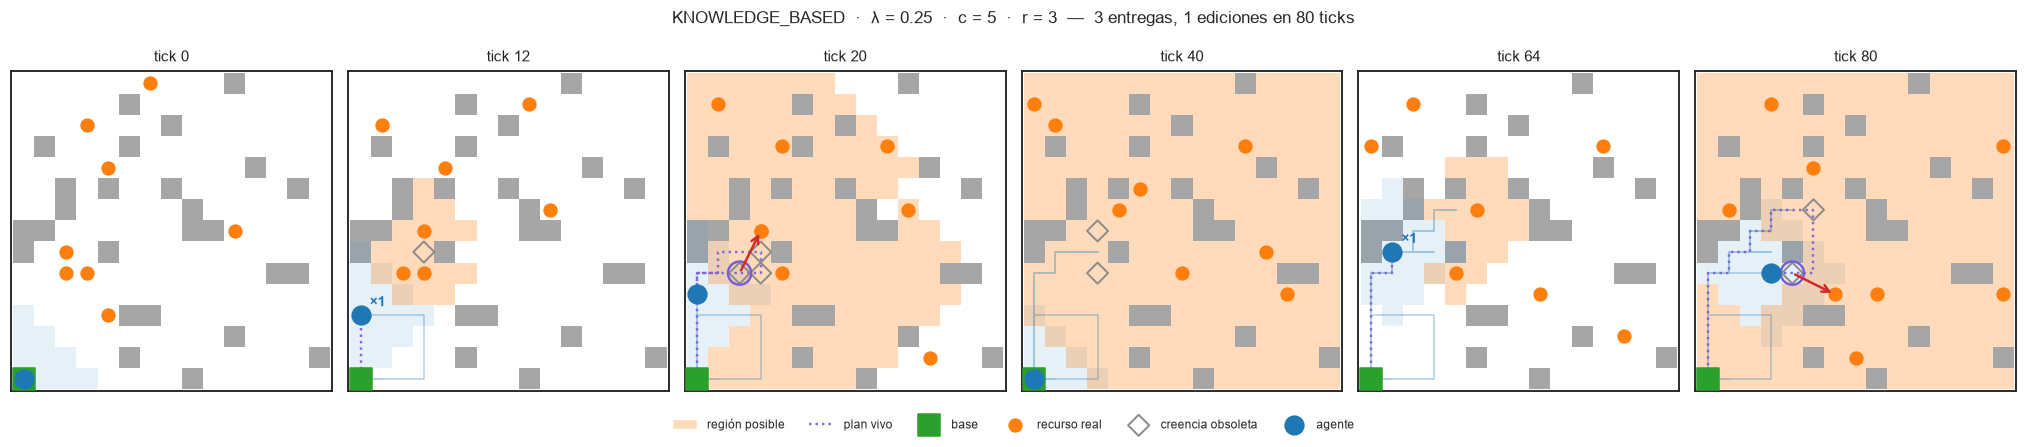
\includegraphics[width=\linewidth]{tira-knowledge-based}
  \caption{Seis instantáneas de una corrida de \KB{} ($\lambda=0.25$, $c=5$, $r=3$, semilla 3). En naranja claro, la región posible de los recursos que el agente rastrea; en naranja, la posición real de cada recurso; el rombo hueco es su última observación y la flecha roja una divergencia. En los 80 ticks el agente delibera 8 ticks, frente a 25 de \CL{} en el mismo mundo (con 3 entregas contra 4, lo cual, en una sola corrida, no dice nada sobre cuál rinde más).}
  \label{fig:tira-kb}
\end{figure}

\FloatBarrier
\subsection{El agente bayesiano}\label{sec:res-bayes}

\BY{} corre en los mismos barridos que \KB, y el cuadro~\ref{tab:bayes} reúne sus contrastes junto con el error final de su estimación de $\lambda$. HB2 pasa sin una sola corrida distinta (cuadro~\ref{tab:controles}), HB3, HB4 y HB5 se confirman, y HB1, que era la hipótesis central de esta extensión, se rechaza.

\begin{table}[htbp]
\centering
\footnotesize
\setlength{\tabcolsep}{4pt}
\begin{tabular}{@{}ll rrrr r@{}}
\toprule
$\lambda$ & $r$ & HB1: \ab{BAY}$-$\ab{KB} & \ab{BAY}$-$\ab{CL} & HB4: \ab{BAY}$-$\ab{MB} & \ab{BAY} \ahora{}$-$\ab{BAY} & Mediana $|\hat\lambda-\lambda|$ \\
\midrule
0.1  & 1        & +2.0 ± 2.6 & +3.0 ± 2.0 & \textbf{+9.7 ± 4.6} & −5.0 ± 3.1 & 0.051 \\
     & 3        & −7.0 ± 6.9 & −4.7 ± 5.7 & +12.3 ± 9.6 & +9.3 ± 6.6 & 0.021 \\
     & $\infty$ & −3.0 ± 5.3 & −3.0 ± 4.8 & \textbf{+38.0 ± 11.9} & +3.0 ± 4.8 & 0.003 \\ \sepfilas
0.25 & 1        & −3.3 ± 2.4 & −2.7 ± 3.1 & +2.0 ± 5.5 & +2.0 ± 2.6 & 0.083 \\
     & 3        & −7.7 ± 6.1 & −2.3 ± 6.0 & \textbf{−32.3 ± 9.1} & −1.0 ± 5.4 & 0.020 \\
     & $\infty$ & \textbf{−14.0 ± 5.5} & +6.0 ± 4.9 & \textbf{−51.0 ± 11.7} & −6.0 ± 4.9 & 0.005 \\ \sepfilas
0.5  & 1        & −3.0 ± 4.5 & +3.3 ± 4.2 & −8.3 ± 5.5 & −6.0 ± 4.8 & 0.080 \\
     & 3        & \textbf{−16.0 ± 4.3} & \textbf{+5.3 ± 2.4} & \textbf{−83.0 ± 10.3} & \textbf{−6.0 ± 2.6} & 0.018 \\
     & $\infty$ & −3.0 ± 2.6 & +2.0 ± 1.4 & \textbf{−117.0 ± 13.8} & −2.0 ± 1.4 & 0.005 \\
\bottomrule
\end{tabular}
\caption{Agente bayesiano ($c=5$). Las cuatro primeras columnas son diferencias pareadas de utilidad; la última, la mediana del error final de $\hat\lambda$, que sobre todo $\lambda$ vale 0.083 con $r=1$, 0.020 con $r=3$ y 0.003 con $r=\infty$.}
\label{tab:bayes}
\end{table}

\begin{itemize}[leftmargin=1.4em, itemsep=0.2em]
  \item \textbf{HB1, rechazada:} \BY{} no supera a \KB{} en ninguna celda, y queda claramente por debajo con $r=3$ y $\lambda=0.5$ (\dif{-16.0}{4.3}) y con visión total a $\lambda=0.25$ (\dif{-14.0}{5.5}), mientras que frente al lazo cerrado queda a la par en casi todo el rango.
  \item \textbf{HB3, confirmada:} La mediana de $|\hat\lambda-\lambda|$ es 0.083 con $r=1$, 0.020 con $r=3$ y 0.003 con $r=\infty$, de forma que con más visión hay más ensayos y $\lambda$ se aprende casi exacto; con $r=1$ y $\lambda=0$ el error mediano llega a 0.134, porque la previa uniforme pesa sobre pocos ensayos. La ley $1/\sqrt{n}$ en sí no se midió, porque el barrido no guarda el número de ensayos de cada corrida.
  \item \textbf{HB4, confirmada:} A $\lambda=0.5$ y $r=3$, \BY{} queda \dif{83.0}{10.3} puntos por debajo de \MB{} (15.3 contra 98.3), de modo que saber cuánto se sabe cierra 5 de los 88 puntos que separan al lazo cerrado de no planificar, menos que los 21 que cierra saber solo qué es posible.
  \item \textbf{HB5, confirmada:} El filtro está calibrado (figura~\ref{fig:fiabilidad}), pues la frecuencia observada sigue la diagonal en todo el rango, la mayor desviación en los intervalos con muchas celdas es de dos centésimas (entre 0.1 y 0.2), y los intervalos altos, con pocas celdas, tienen bandas que alcanzan la diagonal.
\end{itemize}

\begin{figure}[htbp]
  \centering
  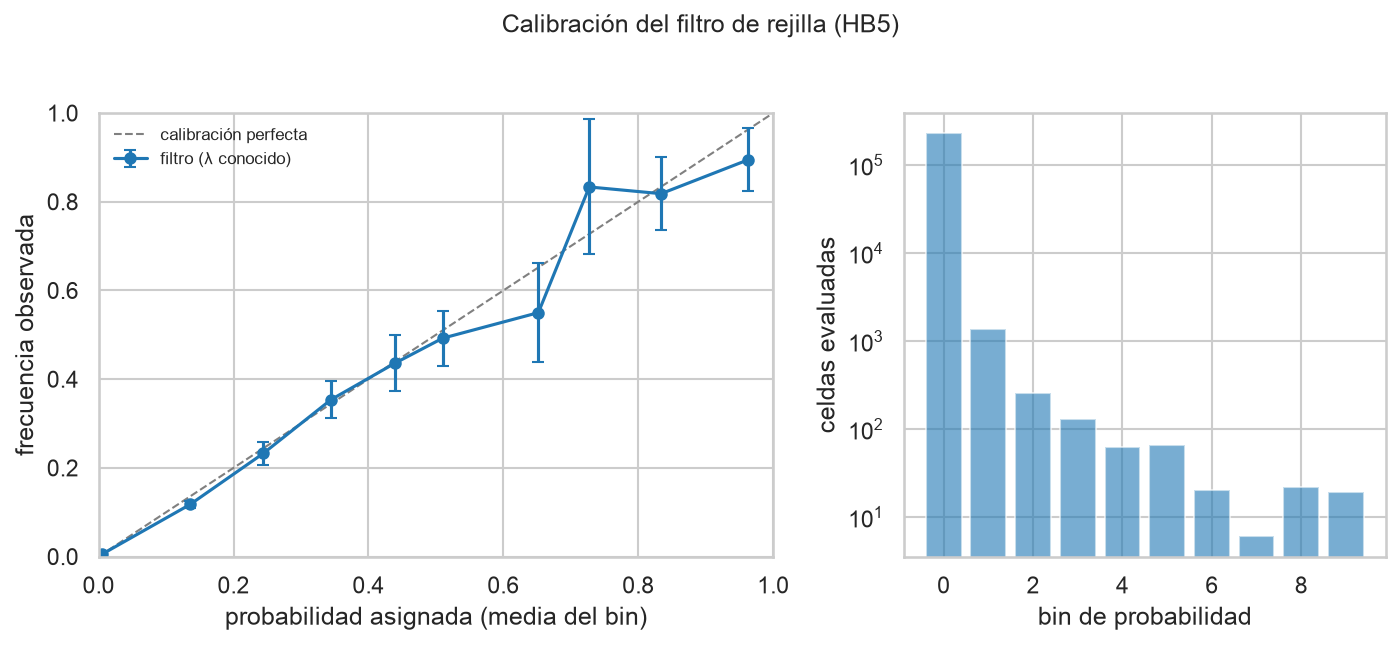
\includegraphics[width=\linewidth]{07-fiabilidad-filtro}
  \caption{Diagrama de fiabilidad del filtro de rejilla (HB5): Seis corridas cortas ($\lambda=0.25$, $r=3$, 300 ticks) en las que un filtro con $\lambda$ conocido incorpora las mismas observaciones que el agente. A la izquierda, la frecuencia con que el recurso estaba en las celdas de cada intervalo de probabilidad asignada, con su error estándar; a la derecha, el número de celdas evaluadas por intervalo, en escala logarítmica.}
  \label{fig:fiabilidad}
\end{figure}

El rechazo de HB1 no viene de la creencia sino de la decisión. Con el horizonte \ahora{} (la ablación, que deja intacta la elección de objetivo y vuelve la decisión de reparar casi idéntica al monitor del cerrado) \BY{} y \KB{} quedan ambos a la par del lazo cerrado, de modo que la diferencia entre ellos con \llegada{} está en la regla de reparación, y el cuadro~\ref{tab:mecanismo} dice en qué dirección: \BY{} repara de forma proactiva bastante más que \KB{} (6.2 contra 2.8 a $\lambda=0.1$ y 16.3 contra 9.5 a $\lambda=0.5$, cerca de las 13.7 del lazo cerrado), pasa más tiempo deliberando (265.1 contra 219.2 ticks a $\lambda=0.5$) y desperdicia más ediciones (145.8 contra 97.4). La regla $c<(1-q)(c+k)$ repara cada vez que el recurso probablemente no volverá a su celda, lo cual es correcto como predicción, pero su contabilidad de costos es incompleta en los dos lados: Por un lado, trata la reparación como si costara $c$ y comprara certeza, cuando el plan reparado nace desactualizado (el mundo sigue moviéndose durante esos $c$ ticks) y una divergencia nueva puede interrumpirlo; por otro, trata un plan mantenido que falla como si costara solo la caminata más $c$, cuando al fallar el agente suele haber perdido además de vista al objetivo, lo cual añade un costo de búsqueda que la regla no modela. La primera omisión empuja a reparar de más y es la que los datos muestran, mientras que la segunda empujaría en sentido contrario, de forma que lo prudente es concluir que, tal como está, la regla repara más de lo que conviene con dinamismo alto, y que la lógica gana justamente porque es más tacaña, pues repara solo cuando $q=0$. Cambiar de horizonte tampoco la arregla: Con \ahora, \BY{} sube de 84.3 a 93.7 a $\lambda=0.1$ (por encima de \KB{} con \llegada, 91.3, pero por debajo de su versión \ahora, 94.7, y dentro del ruido), y baja de 15.3 a 9.3 a $\lambda=0.5$ (\dif{-6.0}{2.6}).

\FloatBarrier
\subsection{Escasez: ¿vale más reparar cuando faltan recursos?}\label{sec:res-escasez}

El número de recursos estuvo fijo en 8 en todos los barridos originales, de modo que el experimento no sabía si el valor de replanificar depende de la abundancia de objetivos. La hipótesis, escrita antes de correr, era que con recursos escasos los viajes entre recogidas son más largos, el objetivo pasa más tiempo expuesto a la deriva y la reparación debería valer más. El barrido se corre en dos regímenes, uno mixto ($r=3$, $c=5$, $p=0.9$) y uno donde replanificar gana ($r=\infty$, $c=0$, $p=1$, el del control 2), y la celda con 8 recursos de cada régimen reproduce exactamente filas que ya existían (figura~\ref{fig:escasez} y cuadro~\ref{tab:escasez}).

\begin{figure}[htbp]
  \centering
  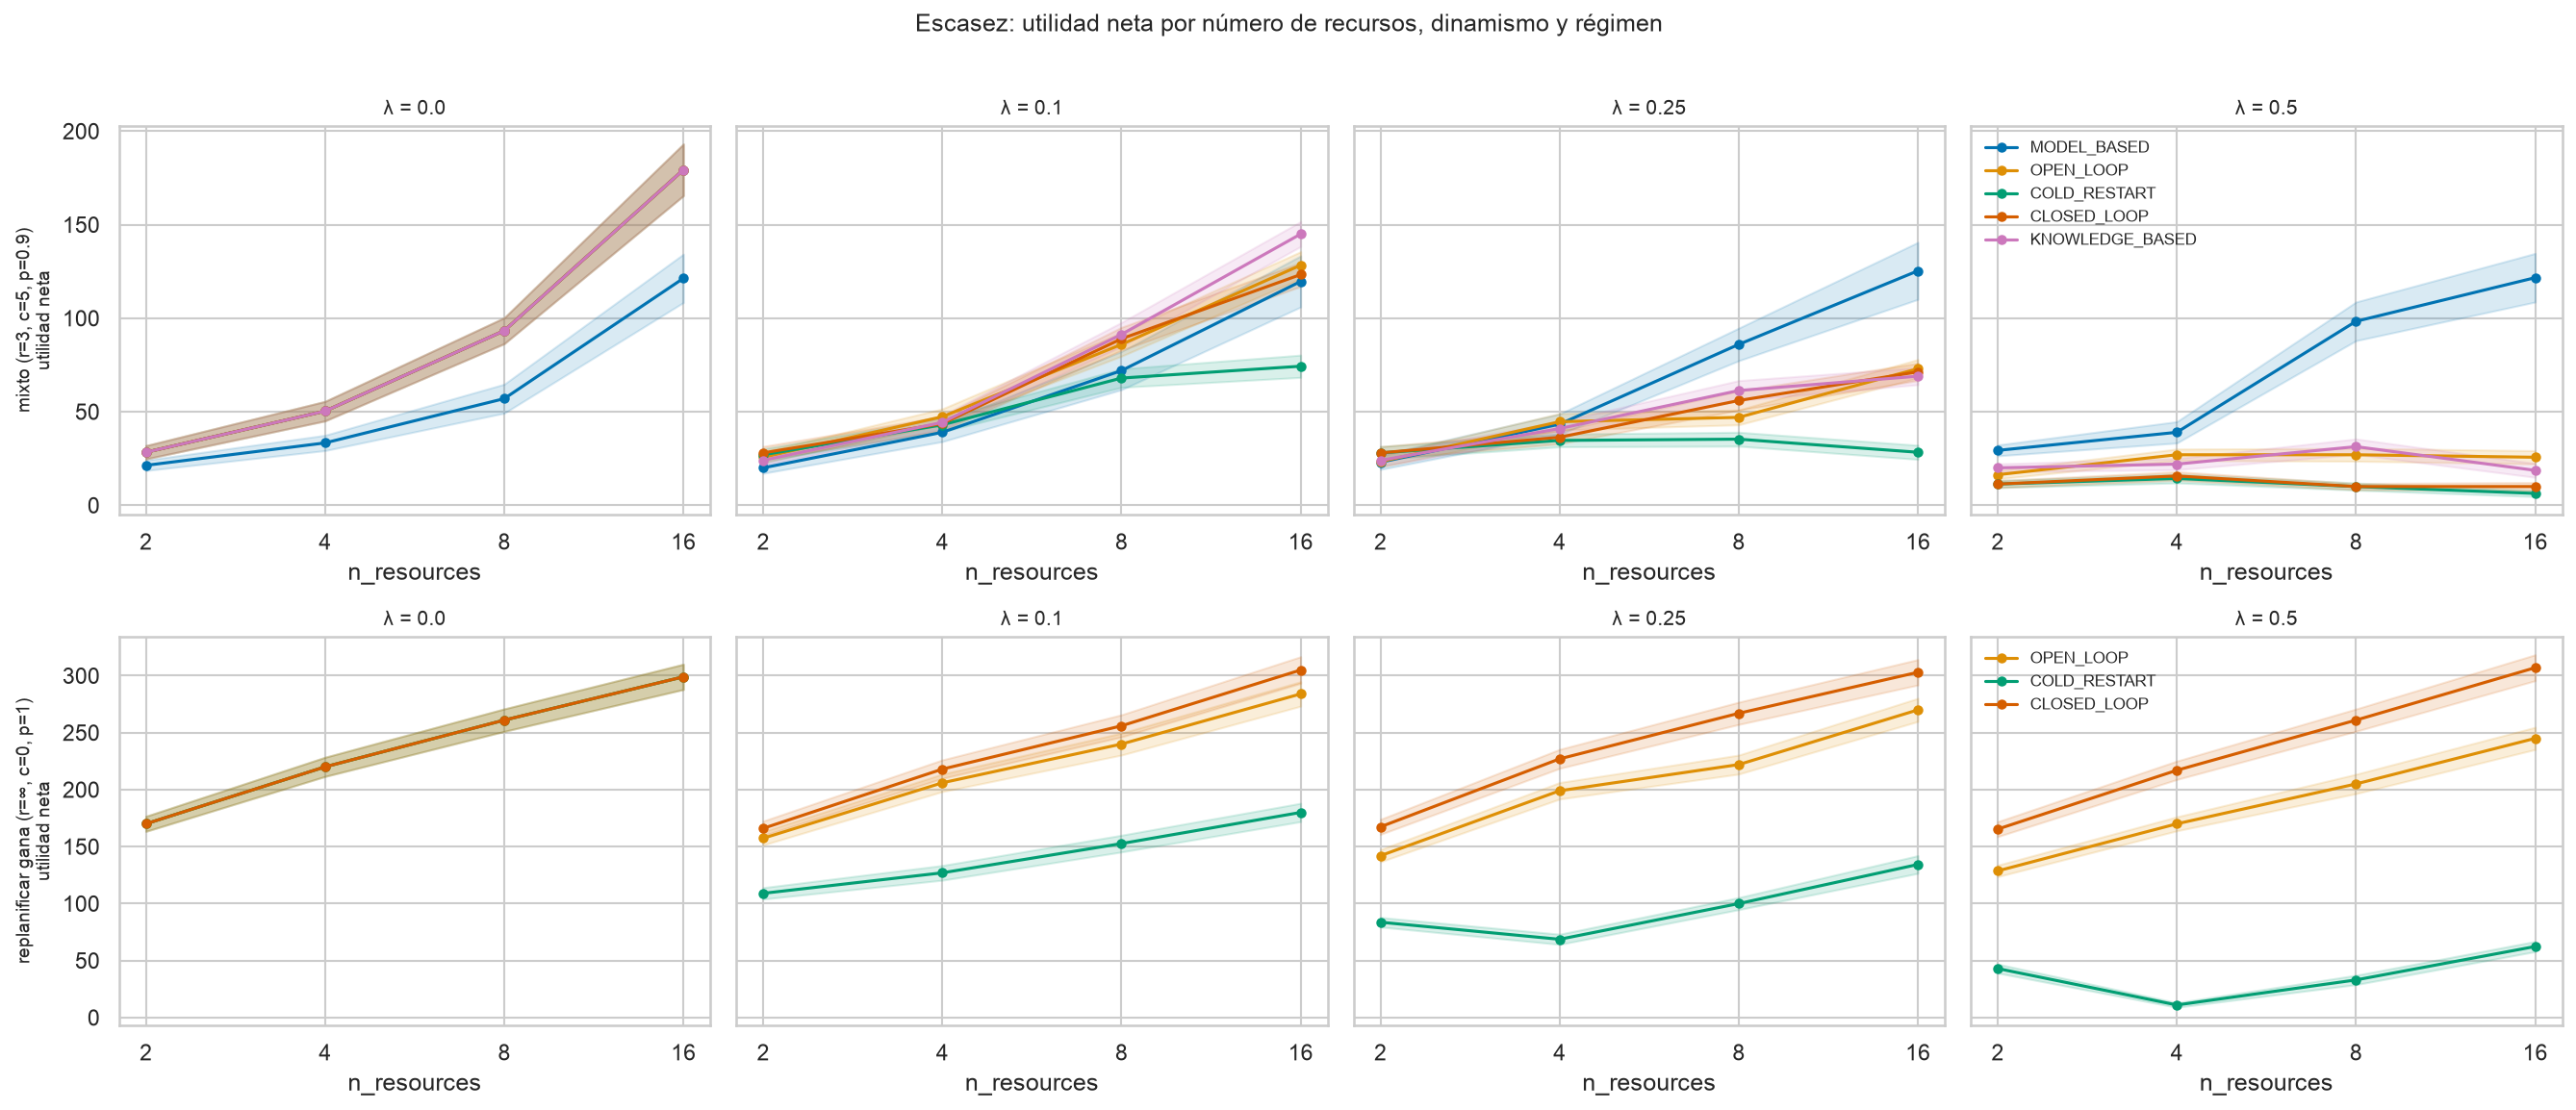
\includegraphics[width=\linewidth]{11-escasez}
  \caption{Utilidad neta por número de recursos $K$, un panel por $\lambda$. Arriba, el régimen mixto ($r=3$, $c=5$, $p=0.9$), donde con $\lambda\ge0.25$ la ventaja de \MB{} crece con la abundancia; abajo, el régimen donde replanificar gana ($r=\infty$, $c=0$, $p=1$), donde la ventaja del lazo cerrado sobre el abierto también crece con la abundancia.}
  \label{fig:escasez}
\end{figure}

\begin{table}[htbp]
\centering
\footnotesize
\begin{tabular}{@{}l l rrrr@{}}
\toprule
Contraste & $\lambda$ & $K=2$ & $K=4$ & $K=8$ & $K=16$ \\
\midrule
\multicolumn{6}{@{}l}{\emph{Régimen donde replanificar gana ($r=\infty$, $c=0$, $p=1$)}} \\
\ab{CL}$-$\ab{OL} & 0.1 & \textbf{+8.7 ± 3.5} & \textbf{+12.0 ± 4.0} & \textbf{+16.0 ± 4.5} & \textbf{+21.0 ± 4.4} \\
\ab{CL}$-$\ab{OL} & 0.5 & \textbf{+36.7 ± 4.0} & \textbf{+47.0 ± 4.0} & \textbf{+56.0 ± 4.3} & \textbf{+62.0 ± 5.0} \\
\ab{CL}$-$\ab{CR} & 0.5 & \textbf{+122.3 ± 6.0} & \textbf{+206.0 ± 7.9} & \textbf{+228.0 ± 9.7} & \textbf{+244.7 ± 10.0} \\ \sepfilas
\multicolumn{6}{@{}l}{\emph{Régimen mixto ($r=3$, $c=5$, $p=0.9$)}} \\
\ab{CL}$-$\ab{OL} & 0.25 & \textbf{+4.7 ± 1.8} & −8.3 ± 4.3 & +9.0 ± 5.7 & −1.7 ± 5.5 \\
\ab{CL}$-$\ab{OL} & 0.5 & \textbf{−5.0 ± 2.4} & \textbf{−11.3 ± 3.9} & \textbf{−17.0 ± 3.8} & \textbf{−15.7 ± 3.6} \\
\ab{CL}$-$\ab{CR} & 0.1 & +1.0 ± 1.0 & +0.7 ± 1.2 & \textbf{+21.0 ± 5.3} & \textbf{+49.0 ± 6.8} \\
\ab{CL}$-$\ab{CR} & 0.25 & 0.0 ± 0.0 & +1.7 ± 1.4 & \textbf{+20.7 ± 5.6} & \textbf{+43.0 ± 5.4} \\
\ab{MB}$-$\ab{CL} & 0.25 & −5.0 ± 3.9 & +7.0 ± 5.1 & \textbf{+30.0 ± 10.1} & \textbf{+54.0 ± 14.8} \\
\ab{MB}$-$\ab{OL} & 0.5 & \textbf{+13.0 ± 3.1} & \textbf{+12.0 ± 5.6} & \textbf{+71.3 ± 9.6} & \textbf{+96.0 ± 13.0} \\
\ab{KB}$-$\ab{CL} & 0.5 & \textbf{+8.7 ± 2.5} & +6.3 ± 3.9 & \textbf{+21.3 ± 3.8} & \textbf{+8.7 ± 3.9} \\
\bottomrule
\end{tabular}
\caption{Diferencias pareadas por número de recursos $K$ en los dos regímenes de escasez. Ninguna fila muestra que reparar valga más cuando los recursos escasean.}
\label{tab:escasez}
\end{table}

La hipótesis se refuta en los dos regímenes, pues reparar vale igual o menos con escasez, no más. Donde replanificar gana, la ventaja del lazo cerrado \emph{crece} con la abundancia, de \dif{+36.7}{4.0} sobre el abierto con 2 recursos a \dif{+62.0}{5.0} con 16 a $\lambda=0.5$, y frente al reinicio en frío de $+122.3$ a $+244.7$. En el régimen mixto el lazo cerrado no saca una ventaja consistente al abierto con $\lambda\le0.25$ en ningún número de recursos, y a $\lambda=0.5$ pierde en todos; reparar en caliente frente a en frío vale cero con 2 y 4 recursos, porque casi no hay carga a bordo que un reinicio pueda tirar (\CR{} pierde a lo sumo 0.5 unidades por corrida), y entre $+43$ y $+49$ con 16 recursos a $\lambda=0.1$ y $0.25$. Lo que sí crece con la abundancia es la ventaja de no planificar, pues a $\lambda=0.5$ la de \MB{} sobre el lazo abierto pasa de $+13.0$ con 2 recursos a $+96.0$ con 16, y a $\lambda=0.25$ su ventaja sobre el cerrado pasa de $-5.0$ a $+54.0$, es decir que la frontera entre deliberar y no deliberar se corre hacia $\lambda$ más bajos cuando sobran objetivos (con 2 y 4 recursos \MB{} solo es la mejor política a $\lambda=0.5$, y con 8 y 16, desde $\lambda=0.25$). \KB, por su parte, mantiene a $\lambda=0.5$ su ventaja sobre el lazo cerrado en toda abundancia, con el signo positivo en los cuatro niveles y fuera del ruido en tres de ellos.

La explicación es la que la hipótesis dejaba escrita para el caso contrario, el costo de oportunidad: Con objetivos escasos el cuello de botella es encontrar y alcanzar un recurso, y un tick deliberando cuesta poco porque de todos modos no había otra entrega cerca, mientras que con objetivos abundantes cada tick quieto es una entrega que se deja de hacer. El mecanismo lo muestra desde el otro lado, pues con más recursos los planes encadenan más objetivos, cada uno es una divergencia posible (a $\lambda=0.5$ el lazo cerrado pasa de 32.8 divergencias reales con 2 recursos a 78.5 con 16) y los ticks deliberando suben con ellas (de 108.6 a 309.8), justo cuando cada tick vale más, de forma que el lazo cerrado entrega lo mismo (alrededor de un recurso) con 2 que con 16 recursos, mientras que \MB{} pasa de 2.9 a 12.2 entregas. Donde deliberar es gratis no hay costo de oportunidad que pagar, y por eso en ese régimen la abundancia favorece a quien repara.

\FloatBarrier
\subsection{Sensibilidad: qué parámetro mueve qué}\label{sec:res-sensibilidad}

Sin correr nada nuevo, los cuatro barridos factoriales originales permiten preguntar qué parámetro mueve más la utilidad de cada política, con el $\eta^2$ de un factor (figura~\ref{fig:sensibilidad}), y lo mismo para la diferencia pareada \OL$-$\CL, que es la pregunta del proyecto (figura~\ref{fig:sens-delta}). Lo que ningún factor explica es interacción entre factores más la variabilidad del mundo que fija cada semilla.

\begin{figure}[htbp]
  \centering
  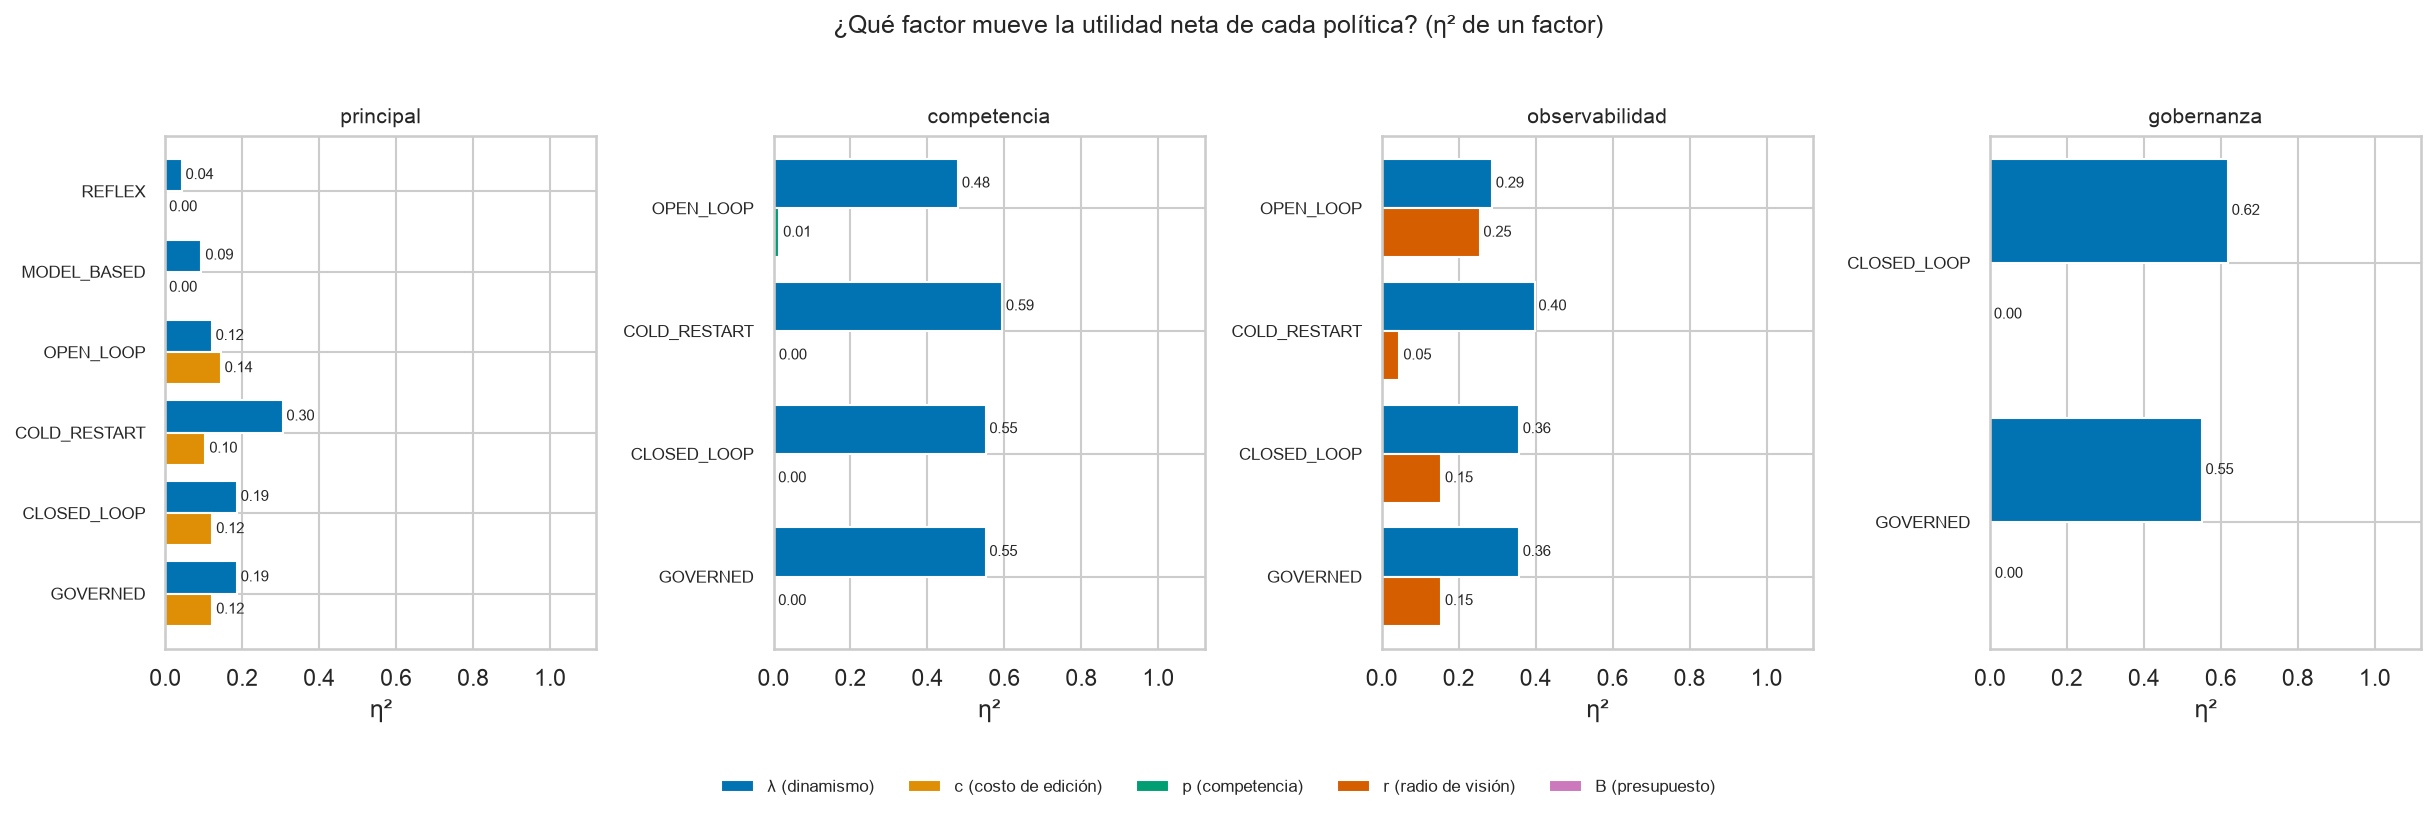
\includegraphics[width=\linewidth]{08-sensibilidad}
  \caption{Fracción de la varianza de la utilidad neta que explica cada factor barrido ($\eta^2$ de un factor), por barrido y por política. $\lambda$ domina en casi todas las políticas con plan; $p$ y $B$ no explican casi nada; \RX{} y \MB{} tienen $\eta^2=0$ para $c$, como debe ser en políticas que nunca deliberan.}
  \label{fig:sensibilidad}
\end{figure}

\begin{figure}[htbp]
  \centering
  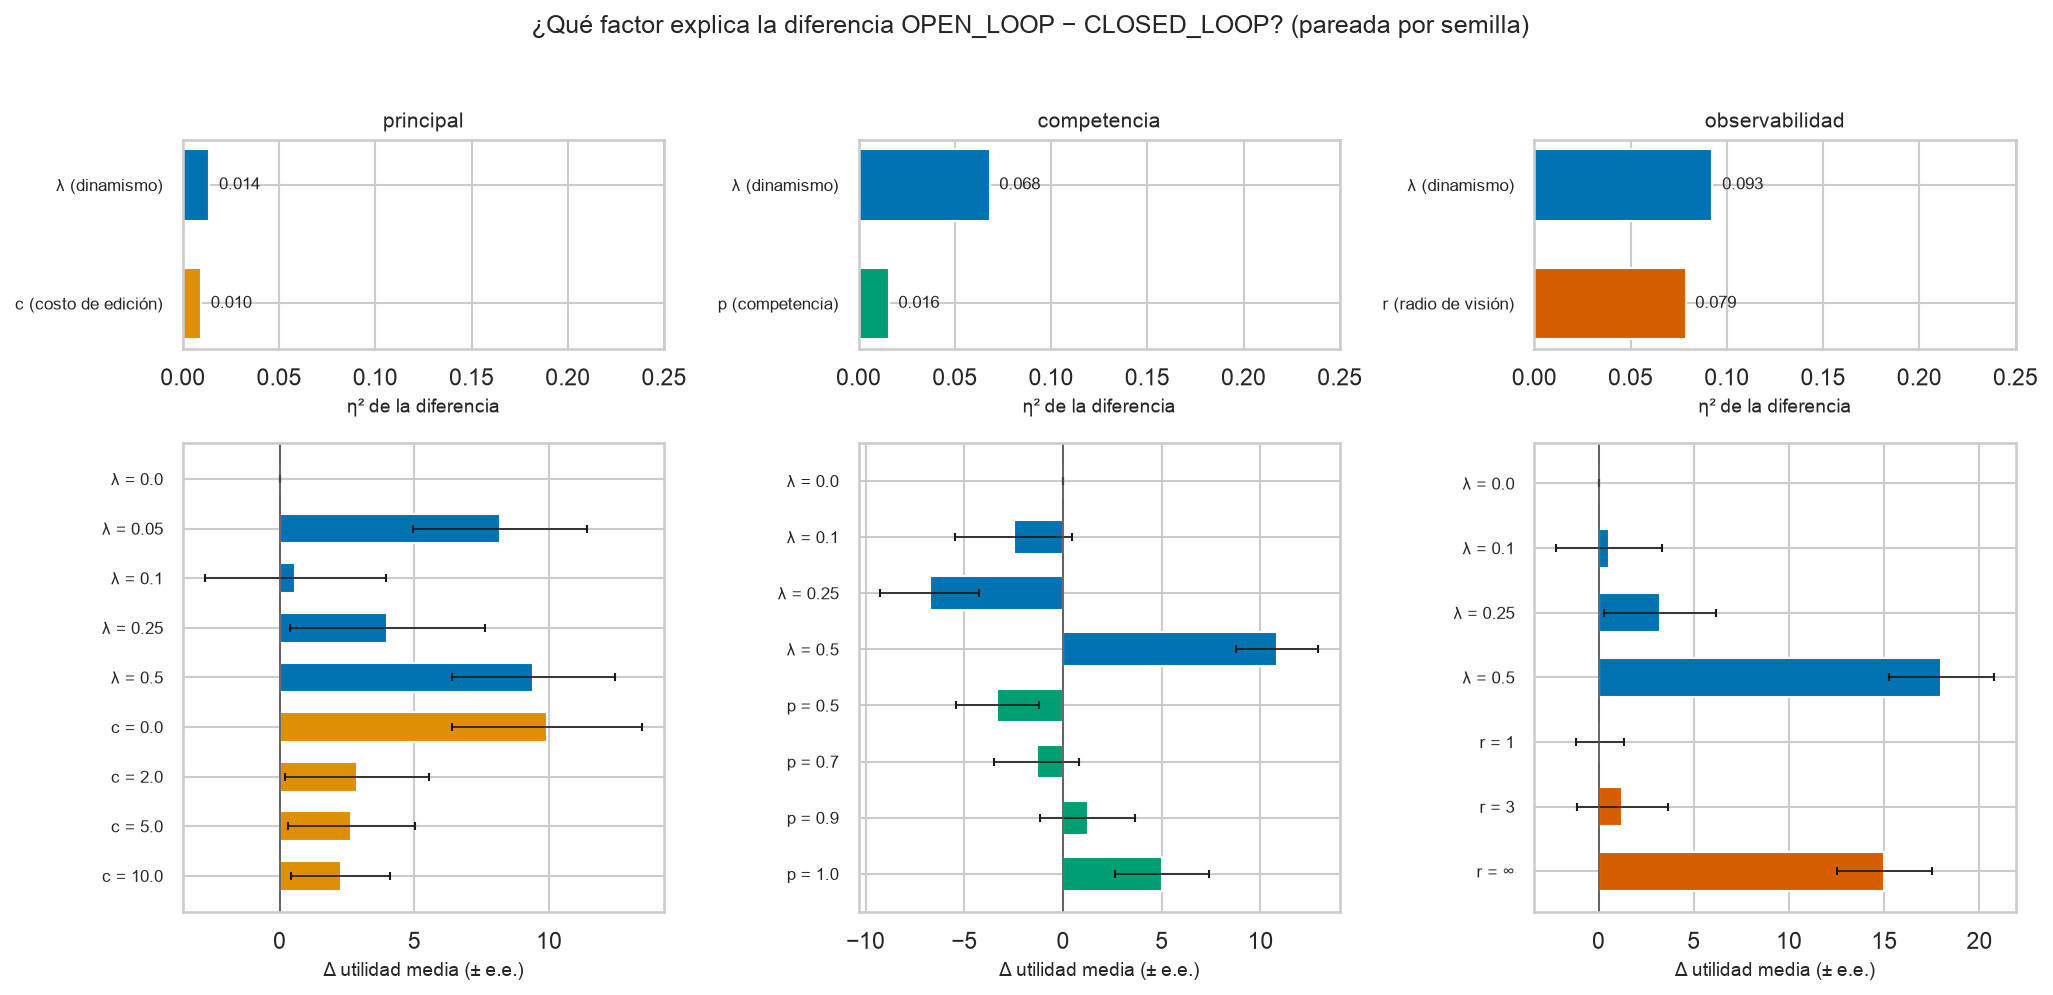
\includegraphics[width=\linewidth]{09-sensibilidad-delta}
  \caption{La misma descomposición sobre la diferencia pareada \OL$-$\CL: Arriba, el $\eta^2$ de cada factor, que no pasa de 0.093; abajo, la diferencia media ($\pm$ EE) en cada nivel, que solo se aleja de cero en los extremos ($c=0$, $\lambda=0.5$ en \texttt{competencia} y $r=\infty$).}
  \label{fig:sens-delta}
\end{figure}

Las tres hipótesis, en orden. Primeramente, $\lambda$ domina a las políticas con plan, con una excepción: En \texttt{competencia}, \texttt{observabilidad} y \texttt{gobernanza} explica entre el 29\,\% y el 62\,\% de la varianza de cada política, muy por encima de $p$ (a lo sumo 1.5\,\%), $r$ (entre 5\,\% y 25\,\%) y $B$ (a lo sumo 0.3\,\%), y en \texttt{principal} domina en \CR{} (0.305 contra 0.104 de $c$) y en \CL{} (0.186 contra 0.122), pero en \OL{} gana $c$ por poco (0.144 contra 0.121). Progresivamente, $c$ no explica más que $p$ la diferencia entre lazo abierto y cerrado, porque ninguno explica casi nada: Todos los $\eta^2$ de \OL$-$\CL{} quedan por debajo de 0.10 (en \texttt{principal}, 0.014 para $\lambda$ y 0.010 para $c$; en \texttt{competencia}, 0.068 para $\lambda$ y 0.016 para $p$), de modo que la mayor parte de su variación es ruido entre semillas y mapas, que es la contraparte estadística de la conclusión de §\ref{sec:res-frontera}; donde sí se mueve es en los extremos, con \dif{+9.9}{3.5} con $c=0$ frente a entre $+2.3$ y $+2.9$ en los otros niveles, y \dif{+15.0}{2.5} con $r=\infty$ frente a $+0.1$ y $+1.3$ con $r=1$ y $r=3$. Finalmente, $r$ mueve el nivel pero poco la diferencia solo a medias, pues explica un 25\,\% de la varianza del lazo abierto y un 15\,\% del cerrado, pero solo un 5\,\% del reinicio en frío, y sobre la diferencia explica un 8\,\%, concentrado en el salto a visión total.

Vale la pena anotar lo que dice el conjunto: En las políticas con plan, los factores barridos dejan sin explicar entre el 38\,\% (\CL{} en \texttt{gobernanza}) y el 74\,\% (\OL{} en \texttt{principal}) de la varianza, que se reparte entre interacciones ($\lambda\times c$ es justamente la frontera) y la variabilidad del mundo, por lo que comparar políticas por pares de semilla no es un lujo. Para la pregunta práctica de qué medir en un despliegue, la respuesta es $\lambda$, que es el parámetro que más mueve a toda política con plan y el que decide entre planificar y no planificar, mientras que $p$ apenas vale la pena medirlo, lo cual la calibración confirma desde otro ángulo.

\FloatBarrier
\subsection{Calibración por ABC de un despliegue}\label{sec:res-abc}

La calibración responde a la pregunta de qué haría un despliegue real con estas curvas. Un motor corre \OL{} (el modo sin monitoreo, que es lo que ejecuta un motor sin reparación en caliente) con $c=5$, $r=3$ y $(\lambda^{*}, p^{*})$ ocultos, y su telemetría da cinco tasas por tick (entregas, tareas fallidas, replanificaciones forzadas, divergencias reales y ticks deliberando), promediadas sobre cinco semillas que no pertenecen a ningún barrido. Contra la tabla de referencia (3.000 muestras de la previa uniforme $\lambda\in[0,0.8]$, $p\in[0.5,1]$), cada estadístico se estandariza por su desviación y se acepta el 5\,\% de muestras más cercano al dato (150), que aproxima la posterior. La recomendación se lee luego en dos etapas: «¿Planificar o no?» se lee de \texttt{principal}, que es el único barrido con políticas sin plan, y si la ganadora planifica, «¿abierto o cerrado?» se lee de \texttt{competencia}. Cabe mencionar que el previo de $\lambda$ llega a 0.8 a propósito, pues con el previo cortado en 0.5 el despliegue con $\lambda^{*}=0.5$ quedaba en el borde y su mediana salía en 0.39, con el precio de que para $\lambda>0.5$ la recomendación extrapola desde la última columna de los barridos.

\begin{figure}[htbp]
  \centering
  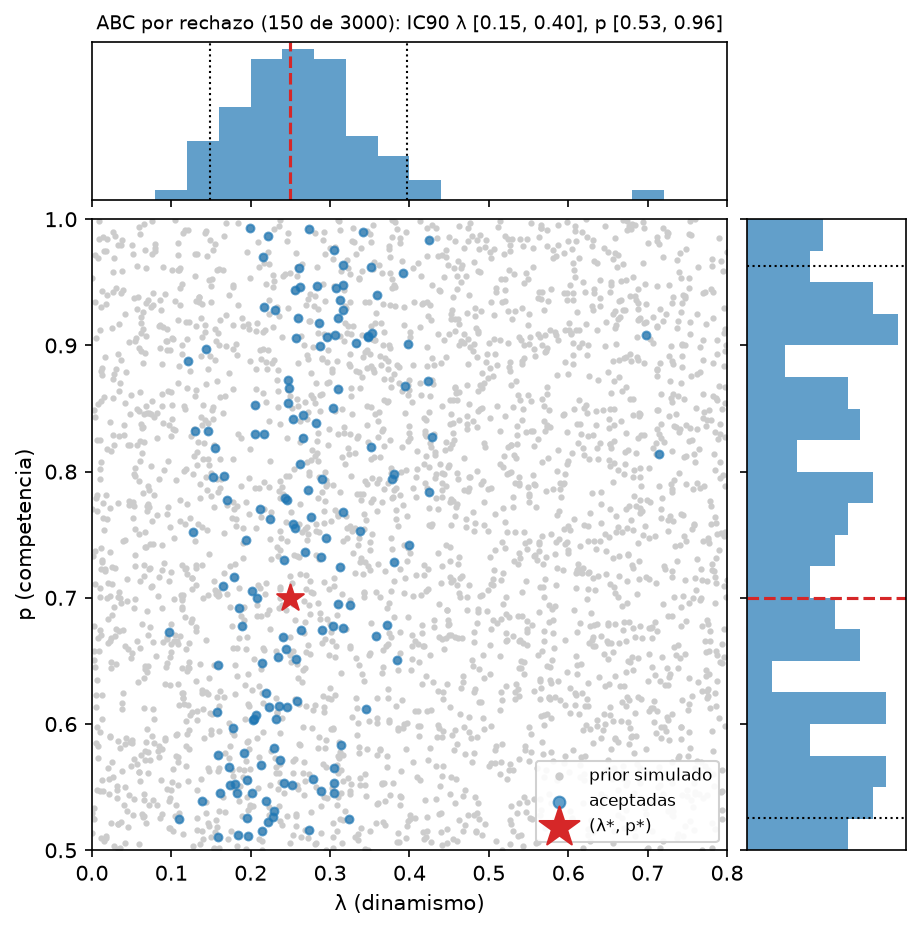
\includegraphics[width=0.62\linewidth]{10-abc}
  \caption{Posterior ABC conjunta del despliegue con $(\lambda^{*}, p^{*}) = (0.25, 0.7)$: En gris las 3.000 muestras de la previa, en azul las 150 aceptadas y la estrella en el valor verdadero; las líneas punteadas de las marginales marcan el intervalo creíble del 90\,\%. La marginal de $\lambda$ se concentra alrededor del valor verdadero, mientras que la de $p$ cubre todo el rango.}
  \label{fig:abc}
\end{figure}

\begin{table}[htbp]
\centering
\footnotesize
\begin{tabular}{@{}l l l L{5.4cm}@{}}
\toprule
$(\lambda^{*}, p^{*})$ & $\lambda$: mediana [IC 90\,\%] & $p$: mediana [IC 90\,\%] & Recomendación combinada \\
\midrule
(0.1, 0.9)  & 0.06 [0.01, 0.14] & 0.76 [0.52, 0.98] & \CL{} 81\,\%, \OL{} 15\,\%, \MB{} 3\,\% \\ \sepfilas
(0.25, 0.7) & 0.25 [0.15, 0.40] & 0.75 [0.53, 0.96] & \MB{} 87\,\%, \CL{} 8\,\%, \OL{} 5\,\% \\ \sepfilas
(0.5, 0.9)  & 0.45 [0.29, 0.74] & 0.75 [0.54, 0.95] & \MB{} 100\,\% \\
\bottomrule
\end{tabular}
\caption{Tres calibraciones de demostración con valores verdaderos conocidos. La recomendación es la fracción de la posterior en la que cada política es la mejor según la frontera barrida. Como referencia, la previa uniforme de $p$ tiene mediana 0.75 y cuantiles del 5\,\% y del 95\,\% en 0.525 y 0.975.}
\label{tab:abc}
\end{table}

La hipótesis se cumple para $\lambda$ y se queda corta para $p$ (cuadro~\ref{tab:abc} y figura~\ref{fig:abc}). Primeramente, $\lambda$ se recupera, pues el valor verdadero cae dentro del intervalo creíble del 90\,\% en los tres casos, con medianas de 0.06, 0.25 y 0.45, aunque la precisión es moderada y empeora con $\lambda$ (los intervalos miden 0.13, 0.25 y 0.45 de ancho). Progresivamente, $p$ no es identificable con esta telemetría, pues las tres posteriores son prácticamente la previa: La hipótesis esperaba una posterior ancha, pero lo que hay es ninguna información, lo cual cuadra con que $\eta^2(p)\le0.015$, ya que un parámetro que casi no mueve el resultado tampoco deja huella en la telemetría que lo resume. Finalmente, la recomendación sí es útil, pues con $\lambda^{*}=0.1$ recomienda planificar, con $\lambda^{*}=0.25$ no planificar (87\,\%) y con $\lambda^{*}=0.5$ no planificar con certeza; la decisión en dos etapas hace falta, porque leída solo en \texttt{competencia}, que no tiene políticas sin plan, la recomendación del caso intermedio sería \CL{} (79\,\%), mientras que \texttt{principal} dice que en ese dinamismo conviene no planificar (87\,\%). Vale la pena leer con cuidado el primer caso, ya que el 81\,\% de \CL{} sale de diferencias con el lazo abierto que quedan dentro del ruido a $\lambda=0.1$, de modo que lo que la calibración respalda ahí es «planificar», más que «monitorear».

\FloatBarrier
\subsection{Balance de las hipótesis}\label{sec:res-balance}

El cuadro~\ref{tab:veredictos} resume el veredicto de cada hipótesis del cuadro~\ref{tab:hipotesis}. Cabe mencionar que cuatro de ellas se rechazaron o no se sostuvieron, y que las dos arquitecturas nuevas dejan dos resultados negativos, lo cual se reporta como resultado y no como fallo del experimento.

\begin{table}[htbp]
\centering
\footnotesize
\begin{tabular}{@{}l l L{11.0cm}@{}}
\toprule
\textbf{Id.} & \textbf{Veredicto} & \textbf{Evidencia principal} \\
\midrule
O1 & Trivial & Con $\lambda=0$ empatan; con $r=3$ no hay umbral a partir del cual reparar al ver la divergencia supere a esperar el fallo (13 de 16 celdas en el ruido) \\ \sepfilas
O2 & Otra frontera & $c$ desplaza el punto desde el cual deja de convenir planificar (\MB{} gana con $\lambda=0.5$, $c\ge2$ y $\lambda=0.25$, $c\ge5$) \\ \sepfilas
O3 & No se sostiene & Control 3 solo por signo; con $p=0.5$ el cerrado supera al abierto a $\lambda=0.25$ (\dif{+11.7}{4.7}) \\ \sepfilas
O4 & En parte & $B=3$ supera a \CL{} a $\lambda=0.5$ (23.7 contra 10.0), pero $B=0$ rinde 27.0; $\eta^2(B)\le0.003$ \\ \sepfilas
O5 & Confirmada & Caliente supera a frío desde $\lambda=0.1$ ($+16$ a $+22$ con $c$ entre 2 y 5) \\ \sepfilas
Orden & Confirmada & Caliente$-$frío y \MB$-$mejor plan conservan el signo en 5 de 6 celdas; abierto$-$cerrado no tiene signo estable \\ \sepfilas
Escasez & Refutada & Reparar vale igual o menos con escasez en ambos regímenes; la explicación es el costo de oportunidad \\ \sepfilas
H1 & A medias & Signo correcto en todas las celdas; fuera del ruido solo con $r=3$, $\lambda=0.5$ (\dif{+21.3}{3.8}); desaparece en la ablación \ahora \\ \sepfilas
H1b & Solo con $\lambda=0.1$ & \dif{+5.3}{4.7} sobre \OL; \dif{-24.7}{9.8} y \dif{-67.0}{10.5} frente a \MB \\ \sepfilas
H2, HB2 & Exactas & 0 de 120 corridas distintas en cada una \\ \sepfilas
H3 & Confirmada & Un tick por consulta invierte el signo; cinco ticks cuestan hasta $-36.7$ \\ \sepfilas
H4 & Confirmada & Más fallos, menos proactivas; ahorro neto de ticks solo a $\lambda=0.5$ (\dif{-63.0}{13.6}) \\ \sepfilas
HB1 & Rechazada & \dif{-16.0}{4.3} frente a \KB{} con $r=3$, $\lambda=0.5$: La regla de utilidad esperada repara de más \\ \sepfilas
HB3 & Confirmada & Error mediano 0.083, 0.020 y 0.003 con $r=1$, 3 e $\infty$ \\ \sepfilas
HB4 & Confirmada & \dif{-83.0}{10.3} frente a \MB{} con $r=3$, $\lambda=0.5$ \\ \sepfilas
HB5 & Confirmada & Diagrama de fiabilidad sobre la diagonal \\ \sepfilas
S1 & Sí, salvo una & $\lambda$ domina salvo en \OL{} dentro de \texttt{principal} ($c$: 0.144 contra 0.121) \\ \sepfilas
S2 & No & Todos los $\eta^2$ de \OL$-$\CL{} $<0.10$: Ni $c$ ni $p$ explican casi nada \\ \sepfilas
S3 & A medias & $r$ explica 25\,\% del nivel del abierto pero 5\,\% del frío; 8\,\% de la diferencia \\ \sepfilas
ABC & A medias & $\lambda$ siempre dentro del IC 90\,\%; $p$ no identificable (posterior $\approx$ previa) \\
\bottomrule
\end{tabular}
\caption{Veredicto de las hipótesis escritas de antemano.}
\label{tab:veredictos}
\end{table}

% !TEX root = ../main-es.tex
%TC:macro \limite [ignore,ignore]
%TC:macro \nota [ignore]
%TC:macro \TODO [ignore]
%TC:macro \parencite [ignore]
%TC:macro \textcite [ignore]
\section{Del Avance 2 al resultado final}\label{sec:avance2}

\subsection{Lo que encontró el Avance 2}

El Avance~2 fue un cuaderno autocontenido con una versión deliberadamente reducida del modelo, cuyo objetivo era aislar el núcleo de la pregunta, el plano $(\lambda, c)$, antes de reintroducir uno a uno los demás parámetros. Conservaba la retícula de $15\times15$ con un 15\,\% de obstáculos, los recursos que derivan con probabilidad $\lambda$, la deliberación que ocupa $c$ ticks mientras el mundo se mueve y el plan calculado con el mundo del inicio de la deliberación, y fijaba todo lo demás: Visión total ($r=\infty$), replanificador exacto ($p=1$), capacidad 1 (sin trabajo en curso), seis recursos, tres políticas (\RX, \OL{} y \CL), 300 ticks y 10 semillas, en un barrido de 600 corridas con $\lambda\in\{0, 0.1, 0.25, 0.5\}$ y $c\in\{0,1,2,5,10\}$. Ambos planificadores ya pagaban el mismo precio por cada reparación, de forma que solo diferían en cuándo invocaban al replanificador. Cabe mencionar que la elección era favorable a la replanificación a propósito, pues visión total más oráculo perfecto es el mejor caso posible para el lazo cerrado, de modo que el resultado funcionaba como una cota superior de lo que reparar al ver la divergencia podía lograr.

Los resultados fueron nítidos. Primeramente, con $\lambda=0$ ambos planificadores obtenían 125 en todo $c$, lo cual confirmaba el control; con $c=0$ el lazo cerrado superaba al abierto a $\lambda=0.25$ (125 contra 118) y a $\lambda=0.5$ (128 contra 114), con un empate práctico a $\lambda=0.1$ (122 contra 123). Progresivamente, al cobrar un solo tick por reparación la relación se invertía en todo el rango, pues con $c=1$ el lazo abierto ganaba a $\lambda=0.1$ (118.1 contra 104.0), a $\lambda=0.25$ (106.2 contra 68.5) y a $\lambda=0.5$ (79.8 contra $-11.3$), de forma que en el caso idealizado el cruce quedaba entre $c=0$ y $c=1$, es decir, la ventaja del lazo cerrado no resistía ni el menor costo de deliberación. El mecanismo estaba en el número de reparaciones, pues el lazo cerrado reparaba ante cada deriva de su objetivo y el abierto solo al fallar (101.3 reparaciones contra 22.2 a $\lambda=0.5$ con $c=1$), y con $c=10$ el lazo cerrado pasaba 289.3 de sus 300 ticks deliberando. Finalmente, el reflejo, que nunca delibera, se mantenía entre 54 y 86 y superaba a ambos planificadores cuando $\lambda c$ crecía (86 contra 27.2 y $-121.4$ con $c=2$ y $\lambda=0.5$).

Vale la pena anotar que los niveles de utilidad del Avance~2 no se comparan directamente con los del modelo final, porque allí la utilidad restaba un punto por cada tick deliberando (es decir, $\kappa=1$, de ahí las utilidades negativas), mientras que en el modelo final $\kappa=0$, y porque cambian la capacidad, el número de recursos y el horizonte. Lo que sí se compara es el sentido de cada efecto.

\subsection{La corrección de la regla de costo}

El cuaderno simplificado del Avance~2 ya cobraba lo mismo a ambos planificadores, pero el modelo completo no lo hacía: Hasta el 2026-10-09, en el modelo completo el lazo abierto replanificaba gratis tras un fallo, con A* exacto y sin consumir ticks, mientras que el lazo cerrado pagaba $c$ y pasaba por el oráculo de competencia $p$ (§\ref{sec:regla-costo}). Al corregir la regla y volver a correr todos los barridos, varias conclusiones de la versión anterior no sobrevivieron:

\begin{itemize}[leftmargin=1.4em, itemsep=0.2em]
  \item \textbf{La dominancia del lazo abierto:} Antes dominaba en todo $\lambda$ y en todo $c$ bajo observabilidad parcial, con ventajas que llegaban a 108 puntos, y esa dominancia era casi entera el efecto de replanificar gratis tras cada fallo; con la regla corregida y $r=3$ el lazo abierto y el cerrado casi empatan (§\ref{sec:res-frontera}).
  \item \textbf{La observabilidad como la variable que lo decide todo:} La lectura anterior sostenía que la observabilidad dominaba el resultado y que con visión total la replanificación ganaba, mientras que ahora la observabilidad mueve sobre todo el nivel de todas las políticas, y con $c=5$ la visión total no hace ganar al lazo cerrado (§\ref{sec:res-observabilidad}).
  \item \textbf{El rescate por presupuesto:} Un \GOV{} con el presupuesto agotado se comportaba como un lazo abierto que replanificaba gratis, de forma que la mayor parte de su aparente rescate del lazo cerrado era el mismo artefacto; ahora el mejor presupuesto a $\lambda=0.5$ es cero (§\ref{sec:res-gobernanza}).
\end{itemize}

La conclusión que sí sobrevivió, y se fortaleció, es la de reparar en caliente frente a reiniciar en frío (a $\lambda=0.1$ con $c=5$ pasó de $+4$ a $+21$ puntos), precisamente porque ahora las dos políticas pagan lo mismo por cada replanificación y lo único que las separa es lo que la comparación quiere medir, el trabajo en curso que una conserva y la otra tira. La lección metodológica es que una asimetría de contabilidad entre las políticas comparadas puede fabricar conclusiones enteras, y por eso el modelo final incluye un control exacto que la vigila, pues con $B=0$ \GOV{} debe ser idéntica a \OL{} corrida a corrida, y lo es en 180 pares sin una sola diferencia.

\subsection{Las cinco hipótesis del siguiente paso}

El Avance~2 cerraba con cinco hipótesis para reintroducir los elementos fijados, cada una contra el caso base idealizado. El cuadro~\ref{tab:avance2} da su veredicto con el modelo final.

\begin{table}[htbp]
\centering
\footnotesize
\begin{tabular}{@{}L{4.6cm} L{10.4cm}@{}}
\toprule
\textbf{Hipótesis del Avance 2} & \textbf{Veredicto con el modelo final} \\
\midrule
1. Con $r$ finito, replanificar sobre una creencia obsoleta degrada al replanificador hasta que comprometerse con el plan resulta mejor & \textbf{A medias:} $r$ mueve sobre todo el nivel, y la diferencia entre abierto y cerrado es casi nula con $r=1$ y $r=3$ (48.0 contra 47.9 y 63.3 contra 62.1) y moderada con $r=\infty$ (\dif{+15.0}{2.5}). La observabilidad parcial no agravó la desventaja del lazo cerrado sino que la diluyó, porque con menos visión detecta, y paga, menos divergencias \\ \sepfilas
2. Con $p<1$ existe una calidad mínima desde la cual conviene auto-editarse & \textbf{No en la forma esperada:} $p$ pesa más sobre quien replanifica menos (de 36.7 a 61.0 en el abierto frente a de 48.3 a 59.7 en el cerrado, a $\lambda=0.25$), explica a lo sumo el 1.5\,\% de la varianza de cada política y no aparece una competencia mínima \\ \sepfilas
3. Con capacidad mayor que 1, reparar en caliente supera a reiniciar en frío & \textbf{Sí:} Desde $\lambda=0.1$ ($+16$ a $+22$ con $c$ entre 2 y 5, $+32$ a $\lambda=0.5$ con $c=0$, hasta $+80.7$ con visión total), salvo donde ambas colapsan; es la conclusión más robusta, también al orden de activación \\ \sepfilas
4. Un presupuesto de ediciones amortigua el \emph{thrashing} & \textbf{Evita el peor caso pero no rescata:} $B=3$ rinde 23.7 contra 10.0 a $\lambda=0.5$ y recorta las ediciones desperdiciadas de 181.8 a 50.7, pero $B=0$ ($\equiv$ \OL) rinde 27.0, y $\eta^2(B)\le0.003$ \\ \sepfilas
5. El barrido completo, con 30 réplicas, ceguera, latencia y el precio $\kappa$, traza la frontera & \textbf{Hecho y extendido, salvo $\kappa$:} 16.260 corridas en trece barridos, más 600 series temporales y 3.000 simulaciones de ABC, aunque todos los barridos se corrieron con $\kappa=0$, de modo que el efecto del precio por tick de deliberar quedó sin medir \\
\bottomrule
\end{tabular}
\caption{Las cinco hipótesis con que cerraba el Avance~2 y su veredicto con el modelo final.}
\label{tab:avance2}
\end{table}

\subsection{Lo que el Avance 2 no anticipó}

El Avance~2 no incluía políticas sin plan más allá del reflejo, por lo que no podía anticipar que la frontera relevante separa deliberar de no deliberar: Con $\lambda$ alto y $c\ge2$ la mejor política es \MB, un agente reactivo que mantiene creencias y nunca paga deliberación, y esa frontera es además la más estable del trabajo, pues sobrevive al orden de activación, aparece desde los primeros ticks y se ensancha con la abundancia de objetivos. Cabe mencionar que la pista estaba en el propio Avance~2, donde el reflejo ya superaba a ambos planificadores cuando $\lambda c$ crecía, aunque entonces se leyó como una curiosidad de la línea base y no como la frontera que buscaba la pregunta.

Tampoco anticipó tres cosas más. Primeramente, que con observabilidad parcial y un replanificador imperfecto el lazo abierto no dominaría al cerrado sino que empatarían, de forma que el cruce idealizado entre $c=0$ y $c=1$ se convirtió, en el modelo completo, en una región amplia donde monitorear el plan no compra nada medible. Progresivamente, que el valor de reparar en caliente no sería monótono en $c$, y que la escasez de recursos, en vez de hacer más valiosa la reparación, la haría valer menos. Finalmente, la promesa con que cerraba el Avance~2 (reportar la frontera con sus cifras e incertidumbres y traducirla en un criterio de cuándo conviene que un agente reescriba su propio plan) se cumple en la sección~\ref{sec:resultados} y en la discusión que sigue, con el pequeño detalle de que el criterio resultó depender mucho más del dinamismo y del costo de deliberar que de la calidad del replanificador.

% !TEX root = ../main-es.tex
%TC:macro \limite [ignore,ignore]
%TC:macro \nota [ignore]
%TC:macro \TODO [ignore]
%TC:macro \parencite [ignore]
%TC:macro \textcite [ignore]
\section{Discusión}\label{sec:discusion}

\subsection{Por qué la frontera tiene esa forma}

La sesión del curso sobre el modelo predador–presa explica la estabilidad de ese sistema diagnosticando primero por qué colapsa y enumerando después los mecanismos que lo sostienen, y la misma estructura sirve para leer la frontera $(\lambda, c)$ como un sistema y no figura por figura, con la advertencia de que el paralelo es una \emph{analogía} y no un mecanismo, pues el modelo no tiene poblaciones acopladas ni ciclos (la dinámica no mostró ninguna oscilación). Cada pieza se rotula entonces como mecanismo o como analogía, y la evidencia sale de los barridos.

\begin{enumerate}[leftmargin=1.6em, itemsep=0.3em]
  \item \textbf{El diagnóstico, deliberar se come el tiempo} (mecanismo). Con $c=0$ el lazo abierto es la mejor política o empata en todo $\lambda$, pero desde $c=2$ y $\lambda\ge0.25$ la mejor pasa a ser \MB, porque en la celda $\lambda=0.5$, $c=5$ el lazo cerrado pasa 282.2 de sus 400 ticks deliberando y el abierto 153.6, y ese impuesto se cobra desde el primer tramo de la corrida. El frente que importa con dinamismo alto deja de ser «comprometerse frente a reparar» y pasa a ser «planificar frente a no planificar».
  \item \textbf{La observabilidad, un desplazador y no el diagnóstico} (mecanismo). El radio mueve sobre todo el nivel de todas las políticas, y la creencia obsoleta existe (el oráculo no puede acertar sin ver el objetivo), pero no es lo que hunde a las políticas con plan, pues las preguntas lógicas que la atacan (descartar candidatos vistos vacíos y elegir objetivo por el peor caso) no compran nada medible por sí solas, según la ablación con \ahora, y lo único que ayuda es dejar de pagar reparaciones, que es otra vez el punto 1.
  \item \textbf{La respuesta con retardo} (analogía con la reproducción lenta del predador; el retardo en sí es mecanismo). Deliberar ocupa $c$ ticks y el plan se calcula al empezar, de modo que llega desactualizado si el mundo se movió mientras tanto. La analogía se rompe justamente aquí, pues en Lotka–Volterra el retardo produce ciclos, mientras que en este modelo no hay retroalimentación del agente sobre el mundo que pueda producirlos, y el retardo se traduce en un impuesto de ritmo constante: Las entregas acumuladas y los ticks deliberando crecen en línea recta.
  \item \textbf{El \emph{thrashing} de replanificación} (mecanismo). Cada divergencia nueva interrumpe la deliberación en curso y los ticks gastados se pierden, lo cual con $r=\infty$, $c=5$ y $\lambda=0.5$ deja al lazo cerrado en utilidad 0.0, frente a 34.0 del abierto, que también delibera tras cada fallo pero no se deja interrumpir por las divergencias.
  \item \textbf{Los amortiguadores} (analogía con el tope de energía del predador). Un presupuesto pequeño recorta el \emph{thrashing} y el horizonte lógico también, pero con dinamismo alto ninguno supera a no reparar de forma proactiva ($B=0$ rinde 27.0 frente a 23.7 con $B=3$, y \KB{} rinde lo mismo que el lazo abierto, \dif{+4.3}{5.3}), de forma que el mejor amortiguador medido es no reparar al ver la divergencia.
  \item \textbf{La capacidad de carga} (analogía con el pasto que se repone). Cada entrega repone un recurso, de forma que el mundo nunca se queda sin trabajo, y la abundancia cambia el valor de replanificar, aunque al revés de lo esperado. La analogía vale solo en que la abundancia fija la escala, pues el mecanismo es el costo de oportunidad (§\ref{sec:disc-oportunidad}).
\end{enumerate}

Dicho en una frase coherente con los datos: Cuando reparar cuesta, el lazo abierto y el cerrado quedan cerca y, con el entorno cambiando rápido, gana el agente que no delibera, tanto más cuanto más abundan los objetivos; la observabilidad parcial mueve sobre todo el nivel; el \emph{thrashing} es real y un presupuesto pequeño o un horizonte lógico lo recortan, aunque con dinamismo alto no reparar de forma proactiva lo recorta igual; y reparar en caliente frente a reiniciar en frío compensa en casi todo el rango con $\lambda>0$, salvo donde ambas políticas colapsan.

\subsection{Un criterio operable de cuándo reescribir}\label{sec:disc-criterio}

La pregunta del trabajo pedía condiciones del entorno, y la respuesta que dan los datos se puede convertir en un procedimiento. El parámetro que hay que medir es $\lambda$, porque es el factor que más mueve a toda política con plan (hasta el 62\,\% de la varianza) y el que decide entre planificar y no planificar, mientras que la competencia $p$ del replanificador pesa poco ($\eta^2\le0.015$). Además, $\lambda$ se puede medir, pues la calibración por ABC lo recupera a partir de la telemetría de un motor que corre en frío (el valor verdadero cayó dentro del intervalo creíble del 90\,\% en los tres casos), aunque con precisión moderada, mientras que $p$ no es identificable con esa telemetría, ya que con un motor que solo replanifica al fallar los errores del replanificador se confunden con el dinamismo, y medirla exigiría etiquetar cada reparación contra la óptima, cosa que esa telemetría no registra. Por suerte, la decisión que más importa depende de $\lambda$ y no de $p$.

Con $\lambda$ estimado y el costo $c$ de cada reparación conocido (en un motor real, la latencia durante la cual el mundo sigue cambiando), la recomendación se lee en la frontera en dos etapas, primero si planificar y después, si conviene, cómo. El cuadro~\ref{tab:criterio} la resume para el régimen barrido ($r=3$, $p=0.9$), con la advertencia de que las unidades de $\lambda$ y $c$ son las del modelo (probabilidad de deriva por tick y ticks por reparación), de forma que llevarlas a un sistema real exige fijar qué es un tick en él.

\begin{table}[htbp]
\centering
\footnotesize
\begin{tabular}{@{}L{3.4cm} L{4.4cm} L{7.0cm}@{}}
\toprule
\textbf{Régimen} & \textbf{Recomendación} & \textbf{Evidencia} \\
\midrule
$\lambda\approx0$ & Planificar & Las políticas con plan casi duplican a las reactivas (93.3 contra 57.0) \\ \sepfilas
$\lambda$ entre 0.05 y 0.1, $c\le5$ & Planificar y reparar en caliente; monitorear o no es indiferente & \MB{} pierde por entre 17 y 44 puntos; caliente supera a frío desde $\lambda=0.1$; \OL$-$\CL{} dentro del ruido \\ \sepfilas
$\lambda\approx0.25$, $c=0$ & Planificar, en lazo abierto & \OL{} 111.7 contra 86.0 del cerrado y de \MB \\ \sepfilas
$\lambda\approx0.25$, $c=2$; $\lambda\approx0.1$, $c=10$ & Zona de indiferencia & \MB{} frente al mejor planificador: \dif{+4.7}{9.4} y \dif{+4.7}{8.8} \\ \sepfilas
$\lambda\approx0.25$, $c\ge5$ & No planificar & \MB{} gana por \dif{+30.0}{10.1} y \dif{+52.3}{9.2} \\ \sepfilas
$\lambda\approx0.5$, $c=0$ & Planificar o no, casi indiferente & \OL{} 120.3 contra 98.3 de \MB{} (\dif{-22.0}{11.2}) \\ \sepfilas
$\lambda\approx0.5$, $c\ge2$ & No planificar & \MB{} gana por entre $+45$ y $+86$ \\ \sepfilas
Visión total, $c=5$, $\lambda\ge0.25$ & Si se planifica, no monitorear & \OL{} supera a \CL{} por \dif{+20.0}{5.1} y \dif{+34.0}{4.5} \\
\bottomrule
\end{tabular}
\caption{Lectura de la frontera como criterio de decisión, con $r=3$ y $p=0.9$ salvo la última fila. Con más objetivos simultáneos la región de «no planificar» se extiende hacia $\lambda$ más bajos (§\ref{sec:res-escasez}).}
\label{tab:criterio}
\end{table}

Llevado a las tres decisiones de diseño que motivaron el trabajo, el criterio dice lo siguiente. Primeramente, construir la reparación en caliente compensa en cuanto el entorno cambia con alguna frecuencia, pues el reinicio en frío pierde entre 16 y 22 puntos desde $\lambda=0.1$, salvo que deliberar sea tan caro que el agente deje de completar tareas, mientras que en un entorno casi estático reiniciar en frío no cuesta nada medible. Progresivamente, un tope fijo de iteraciones no tiene respaldo en los datos como la razón por la que un agente funciona, y lo que corresponde es derivar cuánto deliberar del dinamismo estimado y del costo de cada reparación, lo cual con dinamismo alto y deliberación cara equivale a no deliberar. Finalmente, un presupuesto de ediciones, del que la autorización humana es una versión manual, evita el peor caso cuando el entorno cambia rápido, pero no rescata al agente, de modo que como freno contra el \emph{thrashing} rinde menos que la decisión, anterior, de no reparar al ver cada divergencia.

\subsection{Lógica frente a probabilidad}

Los dos agentes que infieren dejan un resultado con dos niveles. En el de la \emph{creencia}, el puente de la lógica a la probabilidad funciona sin pérdida: El soporte del filtro coincide tick a tick con la región lógica (lo que la KB considera desconocido es exactamente lo que tiene probabilidad positiva), $\lambda$ se aprende mirando y el filtro está calibrado. En el de la \emph{decisión}, en cambio, tener la probabilidad correcta no bastó, porque una regla de utilidad esperada es tan buena como el modelo de costos con que se evalúa, y la regla $c<(1-q)(c+k)$ omite que el plan reparado nace desactualizado y puede interrumpirse, de forma que repara de más con dinamismo alto. La lógica gana entonces por ser más tacaña, ya que solo repara cuando el recurso ya no puede estar en la celda del plan, y esa tacañería es justamente lo que el experimento premia, pues todo lo que gana \KB{} sobre el lazo cerrado viene de no pagar reparaciones (la ablación con \ahora{} lo deja en cero). Dicho de otra forma, el experimento no refuta que la probabilidad sirva para decidir, sino que muestra que el cuello de botella se movió de \emph{qué sé} a \emph{cuánto cuesta lo que hago con lo que sé}. Una regla corregida, que cargara a la reparación la probabilidad de que el plan reparado caduque durante los $c$ ticks que tarda, es la continuación natural, y no se probó.

El agente lógico deja además una respuesta a la pregunta que la sesión de agentes lógicos planteaba sobre qué pasa con la monotonía si el mundo se mueve: La monotonía no se rompe, se indexa por el tiempo. Ninguna oración se retira nunca, pues $\mathit{Visto}(r,c,t)$ sigue siendo verdadera; lo que caduca es la conclusión «está ahí ahora», que pasa de afirmarse a derivarse con el axioma de deriva, y la prueba de solidez dice que esa derivación nunca deja fuera la celda real. La tabla de creencias de las demás políticas, en cambio, borra y sobrescribe sin dejar rastro, y por eso no puede saber cuán vieja es una creencia. Vale la pena anotar, finalmente, la advertencia de H3 para los agentes basados en modelos de lenguaje, en los que «preguntarse si el plan sigue siendo válido» suele ser otra llamada al modelo: En este experimento, razonar solo compensa si es casi gratis frente a deliberar, pues un solo tick por consulta basta para invertir la ventaja.

\subsection{El costo de oportunidad}\label{sec:disc-oportunidad}

La hipótesis de escasez se escribió con una intuición razonable, que con objetivos escasos cada uno vale más y protegerlo con reparaciones debería compensar, y los datos la refutaron en los dos regímenes. La explicación que la propia hipótesis dejaba escrita para el caso contrario es la que se sostiene: Con objetivos escasos el cuello de botella es encontrar y alcanzar un recurso, y un tick deliberando cuesta poco porque de todos modos no había otra entrega cerca, mientras que con objetivos abundantes cada tick quieto es una entrega que se deja de hacer. El mecanismo es doble, pues con más objetivos hay más divergencias posibles y más reparaciones que pagar, justo cuando cada tick vale más. Donde deliberar es gratis no hay costo de oportunidad, y por eso en ese régimen la abundancia favorece a quien repara. La lectura para el diseño es que el valor de la deliberación no es una propiedad del agente ni del entorno por separado, sino de la relación entre lo que cuesta pensar y lo que se deja de hacer mientras se piensa.

\subsection{Relación con la agenda de los agentes auto-evolutivos}

La dimensión \emph{when} de la agenda de los agentes auto-evolutivos \parencite{gao2026selfevolving} pregunta cuándo debe un agente modificarse, y este trabajo ofrece una respuesta acotada y medible para el caso de la reescritura del plan: No conviene reescribir cada vez que el plan y el mundo dejan de coincidir, sino según cuánto cambia el entorno y cuánto cuesta cada reescritura, y con dinamismo alto y reescritura cara conviene no planificar en absoluto. Esa respuesta matiza, en lugar de contradecir, la presentación de \textcite[§11.5]{russellNorvig2020} del monitoreo de ejecución y la replanificación como la respuesta a un mundo que no se comporta como el plan supone, pues monitorear compensa cuando reparar es barato y bueno (el control 2) y deja de compensar en cuanto reparar cuesta tiempo en un mundo que no espera. Es también coherente con que la línea formal sobre procesos parcialmente observables se pregunte cuándo es seguro saltarse una replanificación \parencite{kong2026open}, y le da la razón a \textcite{brooks1991intelligence} en una región del espacio de parámetros, con dos salvedades: El ganador no es puramente reactivo, pues mantiene creencias, y lo que aparece no es una postura general sino una región delimitada por $\lambda$ y $c$.

Para los sistemas de la clase, la abstracción del oráculo deja una lección que sobrevive al cambio de modelo de lenguaje, pues de los dos parámetros del replanificador el que decide es el costo y no la competencia: Una reescritura casi perfecta que tarda lo suficiente para que el mundo cambie durante ella rinde menos que no reescribir, mientras que mejorar la competencia de un replanificador ya razonable mueve poco el resultado. Cabe mencionar que todo esto se midió con $\kappa=0$, es decir, contando solo el tiempo perdido, de forma que con un costo explícito por tokens la frontera se desplazaría todavía más en contra de deliberar, en una magnitud que este trabajo no midió.

% !TEX root = ../main-es.tex
%TC:macro \limite [ignore,ignore]
%TC:macro \nota [ignore]
%TC:macro \TODO [ignore]
%TC:macro \parencite [ignore]
%TC:macro \textcite [ignore]
\section{Límites}\label{sec:limites}

Los resultados valen dentro de las condiciones en que se midieron, y conviene dejar escrito cuáles son, agrupadas según afecten a la validez externa, al alcance de los barridos o a las arquitecturas nuevas.

\subsection*{Validez externa}

\begin{itemize}[leftmargin=1.4em, itemsep=0.3em]
  \item \textbf{Escala:} Un solo agente, una retícula de $15\times15$ y $T_{\mathrm{max}}=400$, por lo que el régimen multi-agente (incluida la extensión de meta-agentes que se consideró en la planeación) queda fuera.
  \item \textbf{Costo en tokens:} Todos los barridos se corrieron con $\kappa=0$, de forma que el único castigo por deliberar es el tiempo perdido y no un costo monetario, y con $\kappa>0$ la frontera se desplaza sin que se haya medido cuánto.
  \item \textbf{Oráculo:} Es una abstracción del modelo de lenguaje con dos modos de fallo, fiel al \emph{tipo} de error (plausible y equivocado) pero no a su distribución real, y su competencia no depende de la dificultad de la reparación.
  \item \textbf{Unidades:} $\lambda$ y $c$ están en unidades del modelo (probabilidad de deriva por tick y ticks por reparación), de modo que llevar el criterio de la sección~\ref{sec:disc-criterio} a un sistema real exige fijar qué es un tick en él, lo cual este trabajo no hace.
  \item \textbf{Calibración sintética:} El despliegue de la calibración por ABC lo genera el mismo modelo que la tabla de referencia, de forma que el ejercicio muestra que el procedimiento identifica $\lambda$ cuando el modelo es correcto, y no que el modelo describa un motor real; la telemetría tiene solo cinco tasas agregadas de un motor \OL{} con $c=5$ y $r=3$ fijos, y para $\lambda>0.5$ la recomendación extrapola desde los barridos.
\end{itemize}

\subsection*{Alcance de los barridos}

\begin{itemize}[leftmargin=1.4em, itemsep=0.3em]
  \item \textbf{Réplicas:} Con 30 réplicas por combinación, buena parte de las diferencias entre el lazo abierto y el cerrado caen dentro del error estándar (la mayor parte de la varianza de esa diferencia es ruido entre semillas), y el control 3 pasa solo por el signo (85.0 contra 87.5), por lo que conviene leerlo como «el lazo cerrado no mejora» y no como «el lazo cerrado empeora». La regla de dos errores estándar, además, no corrige por comparaciones múltiples.
  \item \textbf{Visión total:} Solo se barrió con $c=5$ y $p=0.9$, además del control 2 y del barrido de escasez en el régimen donde replanificar gana (ambos con $c=0$ y $p=1$), de modo que la frontera en $c$ con observabilidad total queda sin trazar, y la inversión entre esos dos puntos no se puede atribuir solo a $c$, porque también cambia $p$.
  \item \textbf{Alcance de edición:} Es fijo (solo la entrega final queda fuera del alcance del agente) y no se varía en ningún barrido, por lo que su efecto sobre el rendimiento no se ha medido.
  \item \textbf{Dinámica y orden, en una rebanada:} Las series temporales solo tienen $c=5$ y $r=3$ y no guardan la latencia de detección, y el orden aleatorio solo sortea si el recolector actúa antes o después de la deriva, en un subconjunto de \texttt{principal} ($\lambda\ge0.1$ y $c\in\{2,5\}$).
  \item \textbf{Escasez:} Se varió solo el número de recursos, mientras que la capacidad de carga del agente (3) y la reposición de cada recurso entregado quedaron fijas, por lo que el análogo del pasto que se agota no se probó.
  \item \textbf{Sensibilidad:} Es un $\eta^2$ de un factor, solo sobre los cuatro barridos factoriales originales, y las interacciones (en particular $\lambda\times c$, que es la frontera misma) no se descompusieron.
\end{itemize}

\subsection*{Las arquitecturas que infieren}

\begin{itemize}[leftmargin=1.4em, itemsep=0.3em]
  \item \textbf{Inferencia gratuita:} Las preguntas de \KB{} y \BY{} no cuestan nada por defecto, y cuando cada consulta se cobra la ventaja se invierte con un solo tick, de modo que el resultado depende de que razonar sea mucho más barato que deliberar, lo cual es plausible para operaciones de conjuntos pero no está garantizado en un sistema real. Además, la equivalencia entre esas operaciones y DPLL se comprobó solo en una retícula de $4\times4$.
  \item \textbf{La regla bayesiana:} Su modelo de costos omite que el plan reparado nace desactualizado y puede interrumpirse, y que un plan fallido deja al agente sin ver al objetivo, y no se probó una regla corregida, de modo que el rechazo de HB1 es el de esta regla y no el de la decisión bayesiana en general. El agente, por otra parte, aprende $\lambda$ pero recibe la forma de la deriva (una vecina transitable al azar).
  \item \textbf{Mecanismos no aislados:} Dos lecturas plausibles quedaron sin una métrica que las confirme, la de por qué la competencia pesa más sobre el lazo abierto (un error le cuesta un viaje completo antes de descubrirlo) y la de por qué, con el orden sorteado, el lazo cerrado pierde frente al abierto.
\end{itemize}

% !TEX root = ../main-es.tex
%TC:macro \limite [ignore,ignore]
%TC:macro \nota [ignore]
%TC:macro \TODO [ignore]
%TC:macro \parencite [ignore]
%TC:macro \textcite [ignore]
\section{Conclusiones}\label{sec:conclusiones}

Las cifras de este trabajo salen de 16.260 corridas hechas con la regla de costo corregida, y varias conclusiones de la versión anterior del modelo no sobrevivieron a la corrección. El cuadro que queda es más matizado que la frontera limpia que se conjeturaba al comenzar, y con 30 réplicas por combinación varias diferencias entre políticas caen dentro del error estándar, lo cual se indica en cada caso, del mismo modo que se indican las hipótesis que los datos rechazaron.

\begin{enumerate}[leftmargin=1.8em, itemsep=0.35em]
  \item \textbf{Con el mismo replanificador al mismo precio, reparar al ver la divergencia y esperar a que el plan falle casi empatan.} Con $r=3$, la diferencia entre \OL{} y \CL{} va de $-9$ a $+26$ puntos y en 13 de las 16 celdas dinámicas queda dentro de dos errores estándar, ningún factor barrido explica más del 10\,\% de su varianza y su signo cambia en la mitad de las celdas al sortear el orden de activación, de modo que monitorear el plan no compra casi nada sobre replanificar solo al fallar.
  \item \textbf{La frontera que sí aparece separa deliberar de no deliberar.} Cuando el mundo cambia rápido y deliberar es caro, el agente reactivo basado en modelo es la mejor política (98.3 a $\lambda=0.5$ contra 53.3 de la mejor que planifica con $c=2$, y 86.0 contra 56.0 a $\lambda=0.25$ con $c=5$), de forma que el costo de reescritura a partir del cual la ventaja se invierte existe, pero es el que hace dejar de convenir planificar (entre $c=0$ y $c=2$ a $\lambda=0.5$, y entre $c=2$ y $c=5$ a $\lambda=0.25$), y el orden de la taxonomía de agentes depende del entorno de tarea. Es la conclusión más estable del trabajo, pues sobrevive al orden de activación, aparece desde el tick 15 a $\lambda=0.5$ y crece con la abundancia de objetivos (a $\lambda=0.5$, de \dif{+13.0}{3.1} con 2 recursos a \dif{+96.0}{13.0} con 16).
  \item \textbf{Reparar en caliente vale claramente más que reiniciar en frío desde $\lambda=0.1$,} con $+16$ a $+22$ puntos a $\lambda=0.1$ y $0.25$ cuando $c$ está entre 2 y 5, $+32$ puntos ($+41$\,\%) a $\lambda=0.5$ con deliberación gratuita y hasta $+80.7$ con visión total, aunque la relación con $c$ no es monótona y la ventaja se anula donde ambas políticas colapsan. Se mantiene positiva con el orden sorteado, pero tarda en pagar (se separa del ruido desde el tick 105 a 130, cuando hay trabajo en curso que perder) y desaparece cuando los recursos escasean.
  \item \textbf{La observabilidad amplifica lo que decide el costo de deliberar.} Ver más sube el nivel de todas las políticas (de 47.0 a 261.0 a $\lambda=0$ entre $r=1$ y $r=\infty$), pero con $c=5$ la visión total no hace ganar al lazo cerrado (114.5 contra 129.5 del abierto, en promedio sobre $\lambda$), que solo domina con deliberación gratuita y oráculo perfecto.
  \item \textbf{Acotar las reparaciones proactivas evita el peor caso, pero no hay una cuota óptima que rescate al agente.} A $\lambda=0.5$, $B=3$ rinde 23.7 contra 10.0 del lazo cerrado, pero $B=0$ (el lazo abierto) rinde 27.0, y el presupuesto explica a lo sumo el 0.3\,\% de la varianza, por lo que un tope fijo y bajo de iteraciones no es la razón por la que el agente funciona.
  \item \textbf{La competencia del replanificador pesa más sobre quien replanifica menos, y en general pesa poco.} Subir $p$ de 0.5 a 1 lleva al lazo abierto de 36.7 a 61.0 a $\lambda=0.25$ y al cerrado solo de 48.3 a 59.7, pero $p$ explica a lo sumo el 1.5\,\% de la varianza de cada política y no deja huella en la telemetría de un motor en frío.
  \item \textbf{Las políticas se separan por ritmo, no por un evento.} Las entregas acumuladas y los ticks deliberando crecen casi en línea recta desde el tick 50, con pendientes que fija $\lambda$, de modo que el \emph{thrashing} es un impuesto constante y no una crisis.
  \item \textbf{Saber qué se sabe ayuda solo cuando evita pagar reparaciones, y no alcanza a no planificar.} \KB{} supera al lazo cerrado con el signo esperado en todo el rango, pero solo fuera del ruido con $r=3$ y $\lambda=0.5$ (\dif{+21.3}{3.8}); la ganancia desaparece en la ablación con horizonte \ahora, queda por debajo de \MB{} desde $\lambda=0.25$, y un solo tick por consulta invierte la ventaja. La monotonía, por su parte, no se rompe cuando el mundo se mueve, sino que se indexa por el tiempo.
  \item \textbf{Saber cuánto se sabe no mejoró la decisión.} \BY{} aprende $\lambda$ (error mediano de 0.020 con $r=3$) y su filtro está calibrado y tiene exactamente el soporte de la región lógica, pero queda por debajo del agente lógico (\dif{-16.0}{4.3} con $r=3$ y $\lambda=0.5$), porque su regla de utilidad esperada repara de más, y 83.0 puntos por debajo de \MB. El puente de la lógica a la probabilidad funciona en la creencia y falla en la decisión, cuyo modelo de costos resultó ser el eslabón débil.
  \item \textbf{Reparar vale menos, no más, cuando los recursos escasean.} Donde replanificar es gratis, la ventaja del lazo cerrado crece con la abundancia (de \dif{+36.7}{4.0} a \dif{+62.0}{5.0} a $\lambda=0.5$), y donde cuesta, crece la de no planificar, lo cual se explica por el costo de oportunidad de cada tick deliberando cuando sobran objetivos.
  \item \textbf{Lo que hay que medir de un despliegue es $\lambda$, y se puede medir.} $\lambda$ es el factor que más mueve a toda política con plan (hasta el 62\,\% de la varianza) y se recupera por ABC desde la telemetría de un motor en frío, lo cual basta para recomendar si planificar o no, mientras que $p$ no es identificable con esa telemetría ni decisivo para la recomendación.
\end{enumerate}

Volviendo a la pregunta, un agente que reescribe su plan al ver que el mundo cambió supera con claridad a uno que mantiene su plan hasta que falla solo cuando reescribir es casi gratis, el replanificador es bueno y el agente ve lo suficiente (con $c=0$, $p=1$ y visión total gana por entre 14 y 56 puntos según $\lambda$), mientras que con un costo de unos pocos ticks y visión parcial ambos casi empatan, y lo que sí vale desde $\lambda=0.1$ es conservar el trabajo en curso al reescribir, es decir, reparar en caliente en vez de reiniciar en frío. La ventaja de deliberar se invierte a partir de un costo de reescritura de unos pocos ticks (desde $c=2$ con $\lambda=0.5$, y entre $c=2$ y $c=5$ con $\lambda=0.25$, en unidades del modelo), pero no a favor del plan estático sino a favor de no planificar en absoluto, de forma que la decisión de cuándo reescribir resulta ser, antes que nada, la decisión de si deliberar, y se toma midiendo el dinamismo del entorno y el costo de deliberar, no la calidad del replanificador.

% !TEX root = ../main-es.tex
%TC:macro \nocite [ignore]
{\emergencystretch=3em
\printbibliography[heading=bibintoc,title={Referencias}]}


\end{document}
